% (atrent) la biblio viene generata senza molti link, prova a compilare
% inoltre c'è errore di compilazione:
%! LaTeX Error: Command \bfseries invalid in math mode.
%See the LaTeX manual or LaTeX Companion for explanation.
%Type  H <return>  for immediate help.
% ...                                                                                               
%l.199 ...lta Xout_{fondo scala}} \cite{art:rif.11}

\documentclass[a4paper]{report} % o article, book, ... È
% packages...
\usepackage{color}
\usepackage{listings}
\usepackage{natbib}
\definecolor{mGreen}{rgb}{0,0.6,0}
\definecolor{mGray}{rgb}{0.5,0.5,0.5}
\definecolor{mPurple}{rgb}{0.58,0,0.82}
\definecolor{backgroundColour}{rgb}{0.95,0.95,0.92}

\lstdefinestyle{CStyle}{frame=tb,
  language=C,
  aboveskip=2mm,
  belowskip=2mm,
  showstringspaces=false,
  columns=flexible,
  basicstyle={\small\ttfamily},
  numbers=none,
  numberstyle=\tiny\color{gray},
  keywordstyle=\color{blue},
  commentstyle=\color{dkgreen},
  stringstyle=\color{mauve},
  breaklines=true,
  breakatwhitespace=true,
  tabsize=2
}


\usepackage[utf8]{inputenc}
\usepackage[english,italian]{babel}
\usepackage[hyphens]{url}
% Bibliografia
\usepackage[autostyle,italian=guillemets]{csquotes}
% \usepackage{biblatex}
% Per generare il file PDF aderente alle specifiche PDF/A-1b. Verificarne poi la validità.
%\usepackage[a-1b]{pdfx}
\usepackage{hyperref}
\usepackage{graphicx}
% Per inserire testo a caso in attesa di realizzare i capitoli
\usepackage{lipsum}
\usepackage{refcheck}
\usepackage[colorinlistoftodos]{todonotes}
\usepackage{url}
%%%%%%%%%%%%%%%%%%%%%%%%%%%%%%%%%%%%%%%%%%%%%%%%%%%%%

\begin{document}
\hypersetup{pageanchor=false}
% Frontespizio
\begin{titlepage}
\begin{center}

\includegraphics[width=\textwidth]{Logo.jpg}\\
{\large{\bf Corso di Laurea Triennale in Informatica}}
\end{center}
\vspace{12mm}
\begin{center}
{\huge{\bf Sperimentazione sul campo}}\\
\vspace{4mm}
{\huge{\bf di rete LPWAN basata}}\\
\vspace{4mm}
{\huge{\bf sul protocollo LoRaWAN}}\\
\end{center}
\vspace{12mm}
\begin{flushright}
{\large{\bf Tesi di Laurea di:}}\\
{\large{\bf Matteo Curti}}\\
{\large{\bf Matr. 802690}}\\
\end{flushright}
\vspace{4mm}
\begin{flushleft}
{\large{\bf Relatore:}}\\
{\large{\bf Andrea Trentini}}\\
\vspace{4mm}
%{\large{\bf Correlatore:}}\\
%{\large{\bf CORREL}}\\
\end{flushleft}
\vspace{12mm}
\begin{center}
{\large{\bf Anno Accademico 2017/2018}}
\end{center}
\end{titlepage}

\tableofcontents


\listoftodos

% o sections (dipende dal documentclass)
\chapter{Cap1}
\section{Sensori e trasduttori}

\todo{(atrent) vedi todo più avanti su come va organizzato TUTTO il testo, quando ho detto che puoi anche citare il 99\% del testo ti ho anche detto che devi mettere qualcosa di tuo che fa da collante, così NON va assolutamente bene, mettere solo il quote non serve a nulla se TUTTO il testo è un quote... deve esserci qualcosa di tuo che tira le fila, vedi esempio minimale (in realtà va scritto qualcosa di più sensato, leggiti un articolo di "state of the art" di qualche argomento e vedrai come vengono realizzati) che ti ho scritto io. Forse è meglio se rimandiamo la tesi alla prossima sessione}


\subsection{I sensori}
\begin{quote}
	I sensori, in un sistema di acquisizione dati, sono le interfacce fisiche tra i dispositivi di elaborazione dei segnali elettrici acquisiti in input e le corrispondenti grandezze fisiche da monitorare in funzione del tempo. 
	
	Un sensore è un dispositivo con la funzione di fornire in uscita un segnale elettrico, sotto forma di tensione o di corrente, del valore teoricamente proporzionale a quello della grandezza fisica in input che si desidera acquisire. 
	
	Per ottenere un segnale elettrico in uscita di un valore linearmente dipendente da una qualsiasi grandezza fisica (temperatura, pressione, forza, flusso luminoso, ecc...) in input, si utilizza il sensore, il cui funzionamento si basa sulla variabilità di una grandezza fisica elettrica, per esempio resistenza, capacità o induttanza, in funzione della grandezza fisica da misurare.
	
	Si definisce caratteristica di trasferimento la curva che rappresenta l'andamento del segnale elettrico generato dal sensore in output in funzione della grandezza fisica in input.
	La caratteristica di trasferimento è il legame che è presente tra la variabile da misurare (ingresso) e il segnale elettrico di uscita dal sensore. 
	Nella pratica accade molto raramente che tale caratteristica di trasferimento corrisponda, anche approssimativamente, alla legge di proporzionalità diretta: 
	\begin{equation}
	V = k \times G
	\end{equation}
	Oppure:
	\begin{equation}
	I = k \times G
	\end{equation}
	dove $V$ è la tensione, mentre I è la corrente fornita dal sensore, $k$ è una costante di taratura e $G$ è la grandezza fisica da acquisire in input. \cite{art:rif.1}
\end{quote}


\begin{figure}
\centering
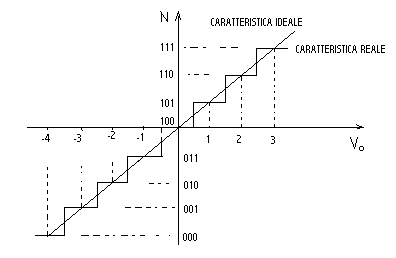
\includegraphics[scale=.8]{Immagini/CarTrasferimento.png}

Fig. 1 Caratteristica di trasferimento ideale vs. reale. \cite{art:rif.19}
\end{figure}

\begin{quote} 
	Generalmente, la caratteristica di trasferimento si allontana, in modo più o meno pronunciato, dal modello ideale a causa di alcuni errori, come l'errore di offset e l'errore di linearità. \cite{art:rif.1} 
\end{quote}

%\todo{(atrent) ad esempio questa frase è copiata integralmente, va quotata, metto esempio di seguito}
%	Generalmente, la caratteristica di trasferimento si allontana, in modo più o
%	meno pronunciato, dal modello ideale a causa di alcuni errori, come l’errore di
%	offset e l’errore di linearità.\cite{...citazione...}

\begin{quote}
	I sensori sono detti lineari la cui caratteristica è una retta. Il funzionamento ottimale di un sensore è definito da una caratteristica lineare. La linearità è il parametro che evidenzia la deviazione tra la retta (caratteristica teorica) e la curva reale. 
	La non linearità è il valore massimo della deviazione rispetto alla curva teorica in valore assoluto riferito al valore massimo del segnale di uscita. Un sensore è buono quando la sua non linearità è inferiore allo 0.1\%. \cite{art:rif.11}
\end{quote}

\begin{quote} 
	L'errore di offset è presente perché il segnale elettrico fornito in uscita è diverso da zero anche quando la grandezza fisica ha valore nullo. Questo avviene quando la retta non passa per l'origine la variabile d'uscita è diversa da zero in corrispondenza del valore nullo della variabile di ingresso. Supponendo che la caratteristica sia lineare:
	\begin{equation}
	V = V_{off} + k \times G
	\end{equation}
	dove $V_{off}$ è la tensione di offset, $k$ è una costante di taratura e G è la grandezza fisica da acquisire in input. Si definisce offset il valore non nullo della variabile di uscita corrispondente al valore nullo della variabile d' ingresso.
	L'errore di linearità è il massimo scarto, in valore assoluto, nel range nominale di funzionamento del sensore tra la caratteristica reale e la caratteristica ideale, dove per caratteristica ideale si intende la caratteristica lineare V, passante per gli estremi della caratteristica reale, nei punti (0, $V_{off}$) e ($F_{max}$, $V_{max}$), dove $F_{max}$ e $V_{max}$ sono rispettivamente il valore massimo della grandezza fisica G ed il valore massimo della tensione V nel range nominale.
\end{quote}

\begin{quote}
	Il range di funzionamento è l'intervallo dei valori che può assumere la grandezza fisica che deve essere trasdotta. Appena la grandezza fisica esce dal range il sensore non funziona più, e ritorna a lavorare appena rientra nell'intervallo. Il range di ingresso (o campo di ingresso) definisce i limiti entro cui può variare il segnale in ingresso; mentre il range di uscita (o campo di uscita) definisce i limiti entro cui può variare il segnale in uscita. \cite{art:rif.11}
\end{quote}   

\subsection{Tipi di sensori}
\begin{quote}
	I sensori si distinguono in base al principio di funzionamento:
	\begin{enumerate}
	\item sensori attivi: se forniscono direttamente un segnale elettrico, in tensione o in corrente, in funzione della grandezza fisica;
	\item sensori passivi: se si utilizza la variabilità di una grandezza elettrica, per es. la resistenza, la capacità o l'induttanza, in funzione della grandezza fisica, per ottenere una tensione o una corrente, inserendo il sensore in un circuito di misura. \cite{art:rif.1}   
	\end{enumerate}
\end{quote}

\begin{quote}
	I sensori si distinguono in base al principio fisico utilizzato:
	\begin{enumerate}
		\item Resistivi: si basano sulla variabilità della resistenza elettrica in funzione degli sforzi meccanici, della temperatura, del campo magnetico, dell'intensità di illuminamento;
		\item Piezoelettrici: si basano sul campo elettrico generato nei cristalli piezoelettrici da sforzi meccanici di trazione, compressione o taglio;
		\item Termoelettrici: si basano sulle forze elettromotrici termoelettriche generate per effetto Seebeck da giunzioni metalliche mantenute a temperature diverse dette termocoppie;
		\item Fotovoltaici: si basano sulle forze elettromotrici generate per effetto fotovoltaico da una giunzione semiconduttrice PN, colpita da radiazioni infrarosse, visibili, ultraviolette, X, $\gamma$ o da particelle cariche;
		\item Fotoelettrici: si basano sulla fotocorrente che si ottiene, per effetto fotoelettrico, nelle celle fotoelettriche a vuoto, nei fotodiodi e nei fototransistor;
		\item Ad effetto Hall: si basano sulle forze elettromotrici generate in particolari materiali, generalmente semiconduttori, percorsi da corrente e sottoposti a campi magnetici;
		\item Capacitivi: si basano sulla variabilità della capacità elettrica di un condensatore in funzione dell'umidità o della costante dielettrica dell'isolante posto tra le armature;
		\item Induttivi: si basano sulla variabilità dell'induttanza di un avvolgimento dotato di un nucleo ferromagnetico estraibile;
		\item Elettromagnetici: si basano sulla legge dell'induzione elettromagnetica.
		\item A riluttanza variabile: si basano sulla variabilità della riluttanza di un circuito magnetico dotato di parti mobili;
		\item Potenziometrici: si basano sulla variabilità della tensione fornita da un partitore potenziometrico regolabile in funzione dello spostamento del cursore;
		\item Piezoacustici e ultrasonici: si basano sulle forze elettromotrici piezoelettriche generate da particolari materiali ceramici sottoposti ad onde meccaniche;
		\item Elettrochimici: si basano sui potenziali elettrochimici generati da celle elettrolitiche speciali, costituite da coppie di elettrodi sensibili a determinati ioni o radicali chimici, oppure sulla variabilità della conducibilità di particolari materiali in presenza di gas o vapori;
		\item Biologici: si basano sulle forze elettromotrici generate da celle elettrolitiche speciali in presenza di enzimi o di altre biomolecole. \cite{art:rif.1}
	\end{enumerate}
\end{quote}

\subsection{Classificazione dei sensori}
\begin{quote}
	La classificazione dei sensori viene fatta in base alle caratteristiche fisiche:
	\begin{enumerate}
	\item resistivi: sfruttano la variazione della resistenza (fotoresistori, termoresistori, sensori di posizione);
	\item capacitivi: sfruttano la variazione della capacità di un condensatore (sensori di umidità);
	\item elettroacustici: convertono segnali sonori in grandezze elettriche (microfoni);
	\item elettrodinamici: si basano sul principio della forza elettromotrice per misurare velocità (dinamo tachimetrica);
	\item elettromagnetici: utilizzano il principio dell'induttanza elettrica per rilevare angoli di rotazione;
	\item magnetostrittivi: si fondano sul principio della permeabilità;
	\item piezoelettrici: sfruttano l'originarsi di una polarizzazione elettrica su facce opposte di cristalli sottoposti a sollecitazioni \\ (stress) fisiche;
	\item semiconduttore: sfruttano le caratteristiche della giunzione dei semiconduttori (fotodiodi, fototransistor). \cite{art:rif.11} 
	\end{enumerate}
\end{quote}

\subsection{I trasduttori}
"Il trasduttore è un dispositivo in grado di trasformare le variazioni di una grandezza fisica,
normalmente non elettrica, in un'altra grandezza, di natura elettrica (tensione, frequenza o corrente). È composto da due parti: sensore e convertitore, un circuito elettronico che trasforma le variazioni di un parametro del sensore in una variazione di una grandezza elettrica" \cite{art:rif.10, art:rif.11}. 

\subsection{Tipi di trasduttori}
\begin{quote}
	I trasduttori sono di due tipi:
	\begin{enumerate}
		\item Analogico: quando il suo segnale di uscita è una grandezza elettrica che varia in modo continuo mantenendo una doppia corrispondenza con il valore della grandezza misurata;
		\item Digitale: quando il suo segnale di uscita è composto da uno o più segnali digitali che possono assumere ciascuno solo due livelli di tensione identificati come 0 e 1.
	\end{enumerate}
	Inoltre i trasduttori possono essere classificati in base alla necessità di energia esterna per il loro funzionamento in:
	\begin{enumerate}
		\item Attivi: Quando forniscono in uscita un segnale direttamente utilizzabile da circuiti di elaborazione senza nessun consumo di energia elettrica;
		\item Passivi: Sono quei trasduttori ai quali bisogna fornire energia elettrica perché la grandezza fisica d'uscita possa essere trasformata in una grandezza elettrica \cite{art:rif.11}. 
	\end{enumerate}
\end{quote}


\begin{figure}
\centering
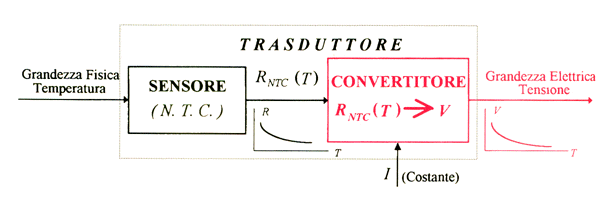
\includegraphics[scale=.7]{Immagini/trasduttore.png}

Fig. 2 Schema di un trasduttore. \cite{art:rif.33}
\end{figure}

\section{Parametri caratteristici}
\subsection{La sensibilità}
\begin{quote}
	La sensibilità è il rapporto tra la variazione della grandezza di uscita $\Delta U$ e la variazione della grandezza d'ingresso $\Delta I$ che la provoca. 
	\begin{equation}
	S = \frac{\Delta U}{\Delta I}
	\end{equation}
	Più il coefficiente angolare della retta è elevato e più il trasduttore è sensibile, e minore sarà il range di funzionamento. Lo strumento risulterà essere molto sensibile quando a parità di grandezza di ingresso la grandezza di uscita è molto elevata.
	Il tempo di risposta è il tempo che il trasduttore impiega per raggiungere in uscita il valore di regime corrispondente al valore d'ingresso \cite{art:rif.11}.
\end{quote}
 
\subsection{La risoluzione}
\begin{quote}
	La risoluzione è il rapporto percentuale tra la minima variazione della grandezza di uscita in grado di essere rilevata e il valore massimo del fondo scala.
	La risoluzione R esprime la variazione minima di uscita rispetto al fondo scala \cite{art:rif.11}:
	\begin{equation}
	R = \frac{\Delta Xout_{min}}{\Delta Xout_{fondo scala}} 
	\end{equation}
\end{quote}
 
\subsection{La riproducibilità}
\begin{quote}
	La riproducibilità è la capacità di un sensore di fornire sempre gli stessi valori di uscita in corrispondenza dell'ingresso. \cite{art:rif.11}
\end{quote}
\begin{quote}
	Vale a dire la costanza nel tempo delle caratteristiche del trasduttore (la sua resistenza all'invecchiamento).\cite{art:rif.17}
\end{quote}
 
\subsection{L'accuratezza}
\begin{quote}
	Nel funzionamento reale il sensore descrive una caratteristica che si discosta dalla funzione ideale
	come in Fig. 1. Per tenere presente la mancata accuratezza del dispositivo, occorre misurare le deviazioni esistenti fra i valori reali e i valori ideali. 
	Le caratteristiche di affidabilità in un trasduttore sono relazionate alla sua vita utile ed a possibili cause di mal funzionamento nel sistema in cui è inserito.
	Infatti, l'accuratezza è la capacità del sensore del trasduttore di espletare la funzione per cui è stato costruito in condizioni prestabilite e per un tempo prefissato. Questo parametro è espresso in termini statistici come la probabilità che il dispositivo funzioni per un tempo o per un numero di cicli specificato. Solo di rado esso è specificato dai costruttori. \cite{art:rif.13}
\end{quote}
\subsection{Il drift}
\begin{quote}
	Il drift è la modifica temporale impredicibile delle caratteristiche del sensore \cite{art:rif.14} 
\end{quote}
e serve a indicare la stabilità sensitiva del sensore del trasduttore a lungo termine. 
\begin{quote}
	La curva di risposta del sensore si modifica col tempo, perché viene introdotto un errore nella misurazione del valore della grandezza in ingresso. Questo errore cresce col tempo. Il drift definisce il tempo di vita della calibrazione del sensore, ovvero quanto tempo usare la stessa curva di risposta. Usare sempre la stessa curva di risposta da luogo ad errori sulle misurazioni non tollerabili. \cite{art:rif.14}
\end{quote}

\begin{quote}
	Il problema della variazione della curva di risposta del sensore nel tempo si risolve calibrandolo dopo una certa quantità di tempo. A seconda dell'importanza della sensibilità del sensore vengono elencate alcune risposte al drift:
	\begin{itemize}
		\item Un controllo di qualità che consiste nel tenere ogni sensore sotto continua osservazione per un lungo periodo (4-6 mesi), durante il quale il sensore viene continuamente ricalibrato per verificarne la stabilità. Solamente così è possibile verificare l'effettiva stabilità nel tempo del comportamento di ogni singolo sensore;
		\item I costruttori di sensori ad alta precisione, come Sea-Bird, scartano i sensori che non dimostrano una buona stabilità durante il periodo di valutazione. In funzione della tecnologia alla base del sensore e della sua costruzione la variazione può essere casuale o lineare e modellabile;
		\item In caso di variazioni casuali della risposta del sensore sono richiesti frequenti calibrazioni per avere misure affidabili;
		\item In caso di variazioni lineari e modellabili sono richieste calibrazioni meno frequenti. Nelle calibrazioni successive si utilizzano termini interpolati \cite{art:rif.15}.  
	\end{itemize}
\end{quote}

\section{Acquisizione e trattamento dei segnali}
\subsection{Il segnale}

\todo{(atrent) modifico il seguente per farti capire come andrebbero scritte tutte le parti prese paro paro}

In \cite{art:rif.2} si definisce il \textit{segnale} come:

\begin{quote}
	``la variazione di una qualsiasi grandezza fisica in funzione del tempo. In generale possiamo affermare che un segnale, sotto opportune ipotesi, può essere descritto matematicamente da una funzione continua.''
\end{quote}

Inoltre, sempre nello stesso testo si aggiunge:
\begin{quote}
	``Le onde di volume viaggiano all'interno della terra e seguono le leggi dell'ottica geometrica. Vi sono due tipi principali di onde di volume:
	\begin{enumerate}
		\item Onde P: (prime) onde di compressione e rarefazione in cui l'oscillazione delle particelle di matteria avviene parallelamente alla direzione di propagazione dell'onda; 
		\item Onde S: (seconde o di taglio) in cui l'oscillazione delle particelle avviene perpendicolarmente alla direzione di propagazione dell'onda.''
	\end{enumerate}
\end{quote}

\todo{(atrent) e via così lungo tutto il testo, cioè DEVE esserci anche del testo tuo che fa da collante, si spera tra l''altro che non sia solo collante formale, cioè che non sia solo una introduzione alla citazione ma che ci sia anche un minimo di commento}


I segnali possono essere di tre tipi:
\begin{quote}
	\begin{enumerate}
		\item Continui o Analogici: quando il loro valore può essere misurato in ogni istante. L'aggettivo "analogico" è usato in relazione al fatto che la loro forma in uscita da un sistema è analoga a quella in ingresso.
		\item Discreti: quando il loro valore può essere misurato solo in determinati istanti di tempo.
		\item Digitali: quando si tratta di segnali discreti la cui ampiezza è associata ad un numero che ne rappresenta il valore in quell'istante. In genere per esprimere il numero viene usata, per semplicità, la base numerica binaria \{0,1\} \cite{art:rif.2}.
	\end{enumerate}
\end{quote}

La teoria dei segnali si suddivide in due grandi branche a seconda del tipo di segnale in esame: 
\begin{quote}
	\begin{enumerate}
		\item Segnali deterministici: quando è possibile prevedere con certezza il suo valore ad un certo istante, che viene determinato una volta conosciuti pochi parametri. Per esempio, una sinusoide di cui sia conosciuta l'ampiezza, la frequenza, e la fase ad un istante dato è un segnale deterministico. 
		\item Segnali aleatori: quando è solo possibile prevedere solamente la probabilità che il segnale assuma un certo valore ad un dato istante. Un segnale aleatorio viene definito completamente da due funzioni, la densità di probabilità e la funzione di correlazione. La prima restituisce la probabilità che il segnale assuma un valore dato, la seconda fornisce una relazione tra i valori del segnale a istanti di tempo diversi.
	\end{enumerate}
	Purtroppo i segnali deterministici non esistono nella realtà, in quanto ogni segnale fisico reale possiede una certa indeterminazione per cui il suo valore non può essere mai previsto con infinita esattezza: risultano però una buona approssimazione in molti casi pratici.
	I casi più importanti dei segnali aleatori sono quelli in cui la distribuzione del segnale è gaussiana e quello in cui il valore del segnale ad un dato istante non è correlato a quello degli istanti precedenti e successivi. Esso prende il nome di rumore bianco \cite{art:rif.2}.
\end{quote}
 
\subsection{Lettura del segnale}
Per leggere un segnale bisogna utilizzare un trasduttore. 
\begin{quote}
	Le caratteristiche importanti che un trasduttore deve possedere sono:
	\begin{itemize}
		\item l'ampiezza del segnale in uscita;
		\item la sensibilità, ovvero il minimo valore misurabile;
		\item la velocità di risposta, ovvero il tempo impiegato dal sensore per fornire una risposta costante dopo una brusca variazione della grandezza da misurare.
	\end{itemize}
	Quest'ultima caratteristica dipende dalla banda passante, ovvero la massima frequenza di variazione del segnale a cui il sensore è in grado di funzionare. 
	Un trasduttore è uno strumento di misura, pertanto la tensione fornita sarà affetta da una piccola componente casuale, che porterà la misurazione a fluttuare intorno al valore medio. Si schematizza questo fenomeno considerando il segnale prodotto dal trasduttore come la somma di una parte proporzionale al segnale vero e proprio che si intende misurare, e da un segnale aleatorio, il rumore bianco \cite{art:rif.2}. 
\end{quote}

\begin{quote}
	Le cause delle fluttuazioni (o sorgenti di rumore) sono molteplici ad esempio:
	\begin{itemize}
	\item la temperatura (rumore termico);
	\item la quantizzazione della carica dell'elettrone;
	\item i campi elettrici presenti nelle vicinanze dell'apparecchio (la linea a 50 Hz);
	\item le vibrazioni meccaniche;
	\item \dots 
	\end{itemize}
	Un ulteriore rumore viene introdotto quando il segnale prodotto dal trasduttore viene trasportato lungo una linea elettrica, o amplificato, o manipolato in qualche modo. \cite{art:rif.2}
\end{quote}

\begin{quote}
	Per permettere ad un calcolatore di elaborare un segnale, bisogna prima convertirlo in un segnale di tipo elettrico. In questo modo è possibile inviare il segnale ad una scheda di acquisizione che trasforma il segnale in una tabella di numeri binari interi, che sono gli unici dati in grado di essere elaborati dal calcolatore, che poi l'utente leggerà come numeri decimali, dopo una appropriata conversione. Si rendono quindi necessarie due distinte operazioni sul segnale: 
	\begin{itemize}
		\item la discretizzazione: consiste nel misurare l'ampiezza del segnale ad intervalli di tempo fissati;
		\item la quantizzazione: consiste nella trasformazione dei valori misurati in numeri interi binari \cite{art:rif.2}. 
	\end{itemize}
\end{quote}
 
\begin{figure}
	\centering
	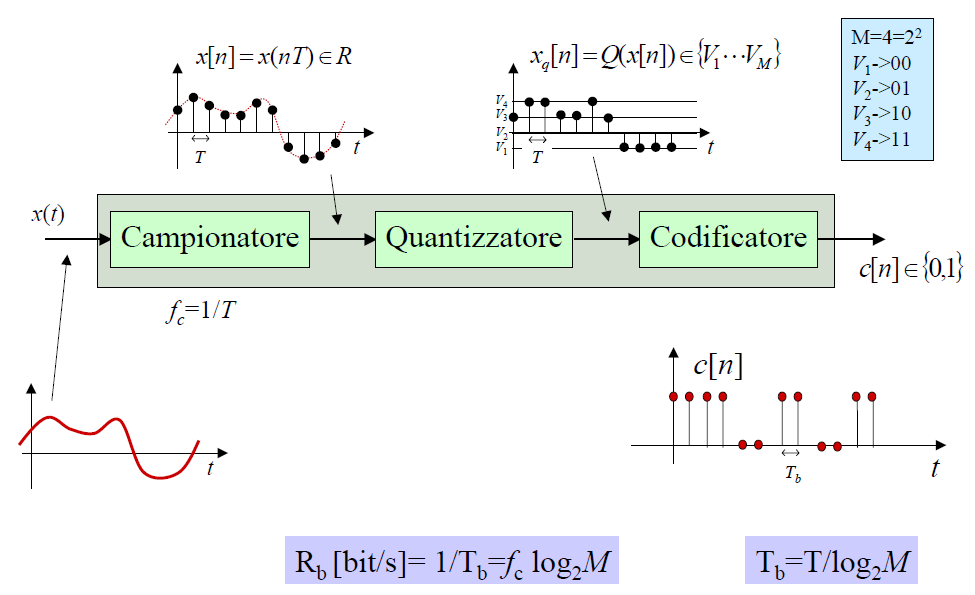
\includegraphics[scale=.4]{Immagini/schemaAD.png}
	
	Fig. 3 Schema a blocchi di un convertitore A/D.
	Materiale didaticco del corso "Fondamenti di segnali e sistemi" \cite{art:rif.7}.
\end{figure}

\begin{quote}
	Il processo di conversione A/D (da analogico a digitale), che trasforma il segnale originario in una sequenza di bit {0,1}, è noto come tecnica PCM (Pulse Code Modulation o modulazione impulsiva codificata). Gli A/D convertono i valori di tensione in ingresso nel numero corrispondente espresso in binario. \cite{art:rif.7}
\end{quote}
 
\subsection{Campionamento o discretizzazione}
\begin{quote}
	La discretizzazione consiste nel misurare l'ampiezza del segnale ad intervalli di tempo fissati. Sia /Delta T l'intervallo di tempo tra due misure successive. La discretizzazione genera un vettore $x$ di dimensione $n$. È evidente che l'intervallo di tempo /Delta T deve essere sufficientemente piccolo da riuscire ad individuare anche piccole variazioni del segnale. L'inverso dell'intervallo /Delta T si chiama frequenza di campionamento ed indica quante volte al secondo viene misurata l'ampiezza del segnale. \cite{art:rif.2}
\end{quote}
  
\subsection{Quantizzazione}
\begin{quote}
	La quantizzazione consiste nella trasformazione delle ampiezze misurate in numeri interi binari ad $N$ bit. Supponiamo che la scheda di acquisizione accetti in ingresso una tensione positiva al massimo di $ V_{0} $ volt. Il numero di intervalli che si possono ottenere con $N$ bit è dato da $2N$, il doppio. Allora il modo più efficiente di convertire il segnale è di dividere l'intervallo $ V_{0} $ in $2N$ sezioni, ciascuna di spessore $ V_{0}/2N $. Dopo di che bisogna assegnare ad ognuna di queste sezioni un numero binario ad $N$ bit. Quando il segnale cade in una di queste sezioni, gli viene assegnato il numero binario corrispondente. Così facendo si commette in ogni misura al massimo un errore pari a metà dello spessore della sezione, $ V_{0}/2N+1 $. La minima variazione rilevabile del segnale in ingresso risulterà essere $ V_{0}/2N $. Ora si suppone che il trasduttore produca in uscita un segnale compreso tra un massimo $ V_{max} $ ed un minimo $ V_{min} $. Visto che la precisione con cui viene quantizzato il segnale dipende solamente dalle caratteristiche della scheda di acquisizione, per ottenere la massima risoluzione è necessario che $V_{max}$ e $V_{min}$ rientrino all'interno dell'intervallo permesso dalla scheda di acquisizione e che vi si adattino al meglio. 
	A questo scopo è necessario amplificare o attenuare il segnale fornito dal trasduttore, ed eventualmente fornire una tensione aggiuntiva per evitare valori negativi. Queste operazioni costituiscono l'esempio più semplice del cosiddetto condizionamento del segnale, che può prevedere anche un filtraggio, la sottrazione di una componente continua, ecc... Molte di queste operazioni vengono effettuate automaticamente dalla scheda di acquisizione stessa. Supponiamo di voler campionare una sinusoide di frequenza $f_{0}$. Intuitivamente, per riuscire ad ottenere un campionamento che rappresenti realisticamente il segnale dobbiamo essere in grado di misurare almeno due volte l'ampiezza del segnale all'interno di un periodo, in modo tale da riuscire ad evidenziare come il segnale oscilli e cambi di segno. Quindi la frequenza di campionamento minima per riuscire a ricostruire il segnale è pari al doppio della frequenza $f_{0}$. In altre parole, se il segnale viene campionato ad una frequenza $f_{s}$, allora sarà possibile campionare correttamente solo i segnali di frequenza minore di $f_{N}=f_{s}/2$. La frequenza $f_{N}$ così definita viene definita frequenza di Nyquist. Un segnale con una certa frequenza, se campionato con una frequenza leggermente superiore, appare con una frequenza molto più bassa di quella reale. Il fenomeno per cui le frequenze maggiori della frequenza di Nyquist vengono riconosciute come frequenze inferiori è detto aliasing. \cite{art:rif.2}
\end{quote}

\begin{quote}
	Per evitare l'aliasing si utilizza un filtro passo basso, che elimina tutte le frequenze superiori a un certo valore (la metà della frequenza di campionamento). Il valore è detto frequenza di cut-off. 
	Sono necessari almeno due campioni per periodo del segnale:
	\begin{enumerate}
		\item la frequenza di campionamento deve essere almeno il doppio della massima frequenza presente nel segnale;
		\item la frequenza di Nyquist. \cite{art:rif.18}
	\end{enumerate}
\end{quote}

\begin{quote}
	Una volta che il segnale è stato campionato, deve essere quantizzata anche l'ampiezza dei valori campionati. Un quantizzatore si occupa di associare ad un range di valori d'ingresso un unico valore di uscita. Questo deve avvenire in quanto, in un segnale analogico, il range di valori tra due estremi è infinito mentre nel mondo digitale solo un certo numero di valori potrà essere rappresentato. La quantizzazione può essere di tipo scalare (SQ) oppure vettoriale (VQ). Nella SQ, ciascun campione viene quantizzato singolarmente, mentre nella VQ vengono quantizzati congiuntamente blocchi di campioni. A sua volta i modi secondo cui il quantizzatore può operare sono diversi, i più comuni sono la quantizzazione uniforme e la quantizzazione a minimo errore quadratico medio. \cite{art:rif.4}
\end{quote}
 
\subsubsection{Uniforme}
\begin{quote}
	Nel caso di quantizzazione uniforme, il gradino $\gamma$ di quantizzazione è uniforme cioè sempre della stessa ampiezza. Questo gradino (detto anche passo di quantizzazione) viene determinato a partire dalla massima dinamica del segnale di ingresso e dal numero di bit che abbiamo a disposizione. Definiamo come $R=[x_{max},x_{min}]$ il range dinamico del segnale di ingresso e come $n$ il numero di bit così da ottenere $\gamma=R/2n$. Ovviamente agendo in questo modo la quantizzazione introduce un errore, detto errore di quantizzazione. In correlazione all'errore di quantizzazione possiamo tenere in considerazione il rapporto tra segnale e rumore di quantizzazione detto SQNR. Esso rappresenta un indice di qualità relativo alla quantizzazione e l'errore di quantizzazione che, inevitabilmente si ottiene quantizzando il segnale campionato. È possibile dimostrare che questo rapporto aumenta di 6 dB per ogni bit aggiuntivo a disposizione della quantizzazione. Questo è intuitivo perché aumentando il numero di bit a disposizione per la quantizzazione, il passo $\gamma$ diventa più piccolo ed il segnale analogico può venire quantizzato in maniera più precisa. Per la descrivere un segnale continuo abbiamo bisogno una sequenza più lunga di valori discreti, quindi sarà maggiore il numero di bit usati e maggiore sarà l'accuratezza della descrizione. Di conseguenza più gradini ci sono minore sarà l'errore di quantizzazione. \cite{art:rif.4}  
\end{quote}

\subsubsection{Non uniforme}
" La quantizzazione non uniforme (o non lineare) slega SQNR e $\gamma$ dinamica. Con non uniforme si indicano intervalli spaziati differentemente ovvero i gradini $\gamma$ non hanno la stessa dimensione." \cite{art:rif.18}

\begin{quote}
	Questa tecnica è utilizzata quando la statistica del segnale in ingresso non è uniforme. \cite{art:rif.7}
\end{quote}

\begin{quote}
	Questo vuol dire che si presentano intervalli più piccoli, e quindi più accurati, dove la concentrazione di valori dei campioni è più alta rispetto a intervalli più grandi e quindi meno accurati, dove la concentrazione di valori di campioni è più bassa. Così facendo si presta più attenzione nella quantizzazione di valori che si presentano con maggiore probabilità diminuendo così l'errore di quantizzazione. \cite{art:rif.6}
\end{quote}

\begin{quote}
	Lo scopo della quantizzazione non uniforme è quello di migliorare l'errore relativo ai bassi livelli del segnale attraverso la quantizzazione non uniforme analogica oppure la quantizzazione non uniforme digitale. 
	Nella quantizzazione non uniforme analogica, il segnale PAM (pulse-amplitude modulation) prima di essere convertito in digitale attraversa un compressore analogico, sostanzialmente un amplificatore logaritmico, che ha lo scopo di amplificare i livelli più bassi del segnale PAM e di comprimere quelli alti. L'apparato ricevente PCM deve contenere un organo denominato espansore, complementare al compressore in grado di ripristinare i livelli originali.
	Nella quantizzazione non uniforme digitale, invece, il segnale PAM è convertito immediatamente in digitale a 12 bit. Successivamente un compressore numerico trasforma i dati in forma seriale a 8 bit. Anche la compressione numerica segue una legge logaritmica simile a quella analogica. L'apparato ricevente PCM deve contenere un organo denominato espansore, complementare al compressore, in grado di ripristinare i livelli originali. Un compressore digitale trasforma una parola a 12 bit (4096 combinazioni) in una a 8 bit (256 combinazioni). La curva del compressore analogico è approssimata con una spezzata costituita, secondo le norme CEPT (Conferenza Europea delle amministrazioni delle Poste e delle Telecomunicazioni), di 8 segmenti ricavati dividendo in 8 parti uguali l'asse delle ordinate. L'asse delle ascisse è così diviso in segmenti chiamati "segmenti di tratta". Dato in ingresso il codice a 12 bit: \\
	$N_{in}$ = [S, N10, N9, N8, N7, N6, N5, N4, N3, N2, N1, N0] \\
	Il compressore numerico fa corrispondere il codice a 8 bit: \\
	$N_{out}$ = [S, A, B, C, D, E, F, G] \\
	Dove $S$ è il bit di segno (0 positivo e 1 negativo), [A, B, C] è il segmento di tratta e [D, E, F, G] è il codice binario corrispondente all'interpolazione lineare dentro la tratta. \cite{art:rif.8}
\end{quote}

\begin{quote}
	La quantizzazione non uniforme è un processo irreversibile, che modifica il segnale originario, approssimandone il valore con uno vicino, ma non identico. Per questo il processo di quantizzazione introduce rumore. Il rumore di quantizzazione in uscita dal filtro di ricezione in un sistema di comunicazione è bianco e gaussiano. \cite{art:rif.6} 
\end{quote}

\begin{quote}
	La non linearità espande gli intervalli più vicini all'origine e comprime quelli verso il valore massimo. 
	Per migliorare le prestazioni in presenza di segnali che possono cambiare significativamente la dinamica bisogna aumentare il numero di bit del campione. Utilizzare quantizzatori non uniformi. Segnali con piccola dinamica vendono piccoli intervalli di quantizzazione, segnali con grande dinamica vedono intervalli di quatizzazione grandi. \cite{art:rif.7} 
\end{quote}

\subsubsection{Logaritmica}
\begin{quote}
	Assegna i valori a regioni uniformi su scala logaritmica.
	\begin{itemize}
	\item Vantaggi: produce risparmi di memoria ed ha una migliore qualità audio a parità di SR (Sample Rate).
	\item Svantaggio: più complesso applicare le tecniche di elaborazione del segnale (la somma di due segnali corrisponde al prodotto, proprietà dei logaritmi). \cite{art:rif.16}
	\end{itemize}
\end{quote}

\begin{quote}
	Gli esempi più importanti di quantizzazione logaritmica sono rappresentati dai quantizzatori A-law e $\mu$-law, utilizzati rispettivamente in Europa e negli USA per la telefonia fissa (PCM, 8000 Hz di campionamento, 8 bit per campione). \cite{art:rif.5}
\end{quote}

\subsection{Codificatore o encoder}
\begin{quote}
	Un codificatore o encoder è un circuito digitale combinatorio dotato di $2^{n}$ segnali di ingresso e di $n$ segnali di uscita. L'attivazione di una delle linee di ingresso produce in uscita il codice corrispondente. Si utilizza in combinazione con i trasduttori digitali che forniscono in ingresso del codificatore un segnale binario. Tra ingresso e uscita del codificatore non esiste però un legame logico, come caso del decoder, perché all'interno di esso esistono delle allocazioni perenni di memoria (memorizzate dal costruttore) tali che il loro numero sia pari alle linee in ingresso (ogni linea attiva individua una locazione di memoria). Se gli ingressi attivati sono più di uno, l'uscita potrebbe assumere una configurazione binaria indesiderata. Per evitare che questo accada, i codificatori in commercio sono possiedono una priorità: se si attiva più di una linea in ingresso, l'uscita assumerà la configurazione associata all'ingresso con priorità maggiore tra quelli attivati. \cite{art:rif.3}
\end{quote}
 
\chapter{Cap2}
\section{Internet of Things}
L'Internet of Things (IoT) tocca tutti gli aspetti della vita quotidiana, coprendo una gamma di applicazioni inimmaginabile, dai dispositivi indossabili connessi, progettati per comunicare su distanze di pochi centimetri, a un'ampia varietà di applicazioni di gestione delle risorse e di monitoraggio a sensori, che potranno comunicare con uno o più gateway su distanze anche di diversi km \cite{art:rif.20, art:rif.21}. 
%% Recentemente, l'acquisizione di dati su vasta scala da dispositivi vincolati si basava sull'approccio M2M (Machine to Machine) che utilizzava comunemente la piena connettività TCP/IP. Tuttavia, lo stack TCP/IP completo spesso non è necessario per le applicazioni IoT incentrate su trasmissioni irregolari, burst di dati di sensori o comandi dell'attuatore. Tali reti sono comunemente implementate utilizzando tecnologie cellulari che introducono elevati requisiti di potenza e costi operativi e quindi limitando drasticamente l'efficienza delle applicazioni IoT, le cui esigenze potrebbero essere soddisfatte dalle capacità relativamente limitate di LPWAN in bande non autorizzate \cite{?}. 
Nel caso in cui siano necessarie comunicazioni a lungo raggio e non possa essere utilizzato un semplice data link wireless senza autorizzazione, le reti cellulari costituiscono un attraente mezzo di collegamento, anche se presentano alcuni inconvenienti. Anche se un dispositivo IoT può essere connesso a basso costo a una rete 2G, con un consumo abbastanza contenuto da poter funzionare con alimentazione a batteria per una durata accettabile, c'è comunque qualche incertezza sul futuro delle reti 2G. Alcuni operatori hanno espresso l'intenzione di abbandonare queste reti, dato che gli abbonati sono orientati ai più moderni servizi 3G e 4G, che garantiscono ai dispositivi mobili un miglior collegamento Internet \cite{art:rif.20, art:rif.21}.
 
%%Però la trasmissione della tecnologia 3G e 4G non è a basso consumo energetico. Inoltre, l'utilizzo di queste tecnologie come modalità di trasmissione si basa in gran parte sulla portante locale della rete, il che significa che la carta SIM deve essere cambiata in diversi paesi \cite{?}. 
I dispositivi IoT si prendono in considerazione per la realizzazione di servizi di lunga durata, dai cinque agli otto anni. Occorre quindi scegliere una connettività di rete che sia sicuramente supportata per una durata di questo periodo. A causa dell'incertezza sulla longevità delle reti 2G, gli sviluppatori devono prendere in considerazione soluzioni alternative di connettività che siano in grado di garantire, non solo la certezza di un supporto a lungo termine, ma anche il rispetto delle esigenze di basso consumo, comunicazioni a lungo raggio e basso costo, tipiche delle più diffuse applicazioni IoT. Fra i possibili candidati, la tecnologia LoRa \cite{art:rif.20, art:rif.21}. 

"Gli investimenti Venture Capital (VC) in questi ultimi anni hanno subito una decisa accelerazione nel settore IoT: a livello mondiale tra il 2010 e il 2015 sono più che raddoppiati passando da 0,8 miliardi di dollari nel 2010, a circa 2 miliardi di dollari nel 2015. A livello cumulativo, il montante degli investimenti in start up specializzate nell’IoT negli ultimi sei anni ha raggiunto la quota di 7,4 miliardi di dollari, per un totale di 887 operazioni. Tra i principali investitori figurano importanti attori del Corporate VC: questo significa che le divisioni di imprese “non finanziarie” hanno l’obiettivo di investire in start up con tecnologie utili al proprio business. Tra gli operatori più attivi sono presenti Cisco Investments, Intel Capital, Google Ventures, GE Ventures e Qualcomm Ventures il cui portafoglio di investimenti in start up specializzate nell’IoT è stato stimato, nel periodo che va dal 2010 al 2015, in circa 3,2 miliardi di dollari. Questi solo alcuni dei dati emersi dal Rapporto Speciale Looking Forward di Accenture, interamente dedicato al tema dell’Internet of Things.
Il percorso di trasformazione digitale in atto nelle imprese e nei mercati apre scenari economici e di business totalmente inediti, attraverso nuovi modelli di apprendimento, collaborazione, “contaminazione” fra imprese, a cavallo tra competizione e gestione. Questo processo interessa al tempo stesso sia le imprese che le istituzioni preposte alla guida dei mercati e dell’economia che devono essere in grado di porre nei tempi adeguati le condizioni infrastrutturali, regolamentari, di formazione per raggiungere in maniera efficace gli obiettivi di crescita diffusa e innovazione. Ad esempio nel 2020 oltre il 35\% della popolazione delle economie mature avrà almeno un dispositivo wearable (indossabile). I consumatori si interfacceranno con ecosistemi digitali e fisici non solo grazie a device tradizionali come PC, smartphone e tablet, ma tramite una moltitudine di oggetti e sensori intelligenti. Questo fenomeno si sposa con l’opportunità di fornire migliori servizi ai consumatori: già oggi infatti il 40\% dei consumatori si dichiara disponibile a condividere dati personali, a patto che questi vengano utilizzati per ricevere servizi disegnati quasi in modo sartoriale. L’applicazione dell’Internet of Things non avrà impatti diretti solo sul cliente finale, ma anche sui processi interni delle aziende volti all’interazione con i clienti stessi. Sensori e oggetti intelligenti posizionati in modo diffuso negli uffici e nei punti vendita consentiranno di ottimizzare i processi di gestione del cliente, favorendo la collaborazione e garantendo un migliore customer service. I grandi operatori della logistica come UPS e DHL stanno già sfruttando le reti di sensori per localizzare e gestire al meglio le loro flotte e per consentire la verifica dello stato di consegna da parte del cliente. Ad esempio in ambito B2B, i produttori di macchinari per movimento terra o attrezzature agricole potrebbero migliorare l’efficienza operativa monitorando in real time le macchine, consentendo anche operazioni di manutenzione predittiva e diminuendo i fermi macchina. 
Non sono però solo le grandi multinazionali ad investire nel comparto dell’Internet of Things numerosi Paesi stanno acquisendo sempre più consapevolezza delle opportunità economiche del comparto, promuovendo numerose iniziative per dare al proprio ecosistema dell’innovazione un ruolo leader che accompagni la società in questa trasformazione tecnologica. E’ quanto sta accadendo in Francia, ad esempio, che ha inaugurato la “Cité de l’objet connecté” ovvero uno spazio di 10.000 metri quadrati messo a disposizione degli startupper per progettare e realizzare oggetti intelligenti e connessi; in Germania l’IoT è stato  classificato come uno tra i settori prioritari in cui concentrare gli investimenti relativi al piano Industry 4.0. La Cina ha investito 800 milioni di dollari per sviluppare il comparto dell’IoT e corposi investimenti vengono portati avanti anche da Corea del Sud e Usa"\cite{art:rif.22}. 
\subsection{Italia e IoT} 
L'Italia "sta attivando diverse iniziative per dare una spinta all’ecosistema dell’innovazione in generale e all’universo dell’IoT in particolare. Secondo la ricerca Accenture “Industrial Internet of Things” l’Italia è uno dei Paesi con le maggiori opportunità di crescita. Lo studio ha evidenziato che investimenti aggiuntivi in questo settore porterebbero a un incremento stimato di produttività  pari a 197 miliardi di dollari entro il 2030.
Inoltre, la vocazione alla tradizione manifatturiera rappresenterebbe un terreno fertile per l’applicazione di tutte le tecnologie di automazione dei processi industriali, per abilitare la fabbrica del futuro (Fabbrica 4.0). Inoltre il posizionamento distintivo e di eccellenza su diversi settori che stanno attualmente guidando la volata all’IoT, come i settori auto, casa, automazione e salute, può essere ulteriore spinta e volano per la trasformazione digitale anche delle filiere legate a tali comparti.
Anche la Pubblica Amminisrazione sembra consapevole della centralità del tema facendo del recupero del gap d’innovazione una priorità strategica per l’Italia che viene confermata da alcuni recenti interventi normativi finalizzati a supportare anche il mercato IoT" \cite{art:rif.22}.

\subsection{SigFox}
Esistono oggi opzioni sempre più interessanti per implementare collegamenti di tipo wireless nelle reti di sensori e in numerose altre applicazioni Internet of Things. Per un decennio o forse più, le reti di telefonia mobile (cellulari) hanno rappresentato l'unica tecnologia di comunicazione wireless universale disponibile per produttori e operatori di apparecchiature M2M (Machine-to-Machine) in grado di garantire una copertura praticamente globale in ogni regione abitata del pianeta. Nel caso delle applicazioni M2M, si è deciso di utilizzare la tecnologia GPRS come base per la connessione alla rete di telefonia mobile, mentre le più recenti tecnologie 3G e 4G (di terza e quarta generazione) garantiscono velocità di trasferimento sempre maggiore a fronte di un aumento dei costi di connessione. Tutte queste tecnologie per telefoni mobili evidenziano svantaggi non indifferenti per gli utilizzatori di apparecchiature M2M: la velocità di trasmissione dati è molto più elevata rispetto a quella richiesta da un gran numero di applicazioni M2M per cui i moduli cellulari integrati nelle apparecchiature IoT sono sovra-specificati e quindi troppo costosi per tali applicazioni. Senza dimenticare che le elevate tariffe che gli operatori di reti mobili impongono per collegare anche il più semplice dei dispositivi wireless sono proporzionali alle elevate velocità di trasferimento dati che la rete può supportare. Un altro aspetto da tenere in considerazione è che le prestazioni offerte dalla tecnologia per telefoni mobili tendono a deteriorarsi in condizioni ambientali severe o estreme. In sintesi, nella maggioranza delle applicazioni M2M, l'utilizzo di una rete di telefonia mobile per garantire la copertura wireless universale risulta costoso. Gli utenti hanno ora la possibilità di scegliere tra due nuove tipologie di reti Wan (Wide Area Network)ciascuna delle quali garantisce sensibili risparmi in termini di costi rispetto alle reti di telefonia mobile. Scopo dell'articolo è confrontare queste nuove tecnologie per applicazioni M2M evidenziando pregi e difetti \cite{art:rif.23}.

\subsubsection{Bassi consumi abbinati a una copertura geografica}
Le reti trattate appartengono alla categoria LPWAN (Low-Power Wide-Area Network) pubblica. Gli approcci di tipo tradizionale alla connettività wireless suggeriscono che un dispositivo di rete non dovrebbe essere in grado di operare con consumi ridotti, mentre sta trasmettendo su lunghe distanze. La topologia delle reti WAN e LPWAN è a stella con una stazione BTS (Base Transceiver Station) al centro, come per la telefonia cellulare. A differenza dei sistemi 2G, 3G o 4G, una rete LPWAN adotta uno schema di modulazione che penalizza la velocità di trasmissione dati (throughput) al fine di garantire una maggiore tolleranza nei confronti delle interferenze e dell'attenuazione del segnale. In questo modo la potenza di trasmissione (in uscita) potrà essere molto bassa. Allo stesso tempo la tecnologia richiede ricevitori caratterizzati da una sensibilità molto elevata al fine di mantenere una connessione in presenza di segnali in ingresso relativamente deboli. Una rete LPWAN è ottimizzata per l'utilizzo in applicazioni M2M e IoT, che richiedono bassi consumi e ridotta velocità di trasferimento dati, a differenza della telefonia mobile. Una cella LPWAN può garantire un'ampia copertura, persino superiore rispetto a quella di una cella di telefonia mobile, utilizzando una potenza inferiore \cite{art:rif.23}.

\subsubsection{Due possibili tecnologie}
Le nuove tecnologie LPWAN operano a frequenze comprese nelle bande ISM esente da licenze. A differenza degli operatori di reti di telefonia mobile, gli operatori di reti LPWAN non devono acquistare costose licenze per l'assegnazione di bande dello spettro radio. Il costo per creare un'infrastruttura wireless pubblica è in ogni caso notevole e il tempo richiesto per raggiungere un grado di copertura tale da permettere alle nuove reti LPWAN pubbliche di soddisfare le esigenze di una vasta platea di utenti è considerevole. Le due tecnologie LPWAN sono SigFox e LoRa \cite{art:rif.23}. %una tecnologia Lpwan sviluppata da Semtech, azienda produttrice di semiconduttori%

\subsubsection{Reti pubbliche SigFox}
"La rete pubblica SigFox copre Francia, Spagna, Gran Bretagna e Paesi Bassi e a partire dal mese di luglio del 2015 sono state condotte numerose prove sul campo in numerose città in tutto il mondo, mentre l'installazione di una rete su scala nazionale è stata avviata in Portogallo, Danimarca, Belgio e Stati Uniti. L'obiettivo di SigFox prevede la copertura su scala nazionale in oltre 60 Paesi entro il 2020. In Francia, SigFox possiede e gestisce la rete, sviluppa l'ecosistema locale e vende abbonamenti ai servizi di comunicazione, mentre in altri Paesi queste attività sono demandate alla responsabilità di partner SNO (SigFox Network Operator). Gli operatori SNO forniscono un servizio di comunicazione end-to-end che trasferisce in modo sicuro i dati dai dispositivi remote agli application server degli utilizzatori. Esso offre un'interoperabilità nativa e il supporto per il roaming, elementi critici per garantire la connettività su scala globale dei dispositivi IoT. Grazie alla topologia tipica della tecnologia SigFox e alla propagazione del segnale su lunghe distanze, l'investimento richiesto per implementare una rete SigFox è molto minore rispetto a quello necessario per i sistemi cellulari tradizionali, consentendo in tal modo agli operatori SNO di fornire la connettività agli utenti OEM (original equipment manufacture) a prezzi accessibili. Un OEM che desidera abbonarsi alla rete pubblica SigFox deve disporre di un modulo client che fa girare lo stack client SigFox e un transceiver radio operante a 868MHz in grado di effettuare la modulazione Dbpsk(Differential Binary Phase-Shift Keying) per l'uplink la modulazione Gfsk (Gaussian Frequency Shift Keying) per il downlink. Alcuni OEM potrebbero decidere di sviluppare in proprio il progetto o il modulo mentre molti altri opteranno per un modulo Cots già pronto all'uso certificato SigFox Ready. I gateway e tutto il software per il collegamento in rete e applicativo per il trasporto dei dati sono forniti da SigFox al fine di assicurare la medesima qualità di fruizione indipendentemente dal Paese in cui gli oggetti stanno comunicando. Poiché secondo SigFox la distanza di trasmissione in campo aperto può essere superiore a 15 km, è possibile creare una rete con copertura universale utilizzando un numero relativamente ridotto di celle. Più stazioni base possono ricevere e trasmettere lo stesso messaggio: questa diversità in ricezione nativa abbinata alla reiezione dell'interferenza dei segnali a banda ultra-stretta (UNB – Ultra Narrow Band)contribuisce a garantire un'elevata affidabilità della trasmissione. La ridotta spaziatura tra i canali nella trasmissione in uplink (ovvero verso la rete) implica un'elevata selettività della stazione base. Questa è resa possibile dall'adozione di ricevitori Sdr (Software-Defined Radio) cognitivi (che cioè effettuano una scansione dinamica dello spettro radio). In questo modo è possibile ridurre la complessità del modem del prodotto finale, che per l'OEM si traduce in una riduzione dei costi di implementazione. SigFox non utilizza uno schema di modulazione proprietario per cui produttori di semiconduttori e costruttori di moduli possono realizzare trasmettitori e transceiver conformi alle specifiche SigFox. Un esempio è rappresentato dalla famiglia di prodotti SigFox compatibili della famiglia ATA8520x di Atmel, la quale ha anche annunciato l'introduzione di un transceiver RF SigFox completamente integrato. I moduli SigFox di tipo Cots sono caratterizzati da una sensibilità massima pari a -126dBm. La potenza di uscita irradiata per la banda ISM è stata stabilita da ETSI (European Telecommunications Standards Institute) ed è pari a 14dBm" \cite{art:rif.23}.

\subsubsection{SigFox: prestazioni, costi e limitazioni}
"In un sistema SigFox il numero di trasmissioni giornaliero è limitato a 140 messaggi in uplink, ciascuno composto da un massimo di 12 byte, e a soli 4 messaggi in downlink, composti da un massimo di 8 byte. La latenza è dell'ordine di 3-5 ms. Sulla base di queste caratteristiche, SigFox è adatta all'uso in applicazioni che prevedono una trasmissione occasionale di piccoli pacchetti di dati, in cui quindi il sistema resta per lunghi periodi in uno stato di inattività (power-down) al fine di preservare la durata della batteria. I contatori per la contabilizzazione dei consumi sono un ottimo esempio di un tipico esempio di una rete SigFox. Gli utenti di SigFox devono pagare una quota annuale per ciascun nodo per la fornitura dei servizi di comunicazione di rete. Questa quota annuale è determinata dagli operatori di rete in ogni Paese ma SigFox sottolinea che in ogni caso gli utenti possono beneficiare di prezzi estremamente competitivi abbinati a consumi di potenza minimi. Il percorso che ha portato allo sviluppo della rete LoRA (abbreviazione di Long Range) universale è differente da quello seguito da SigFox" \cite{art:rif.23}.
In conclusione, SigFox si distingue come una tecnologia a banda ultra-stretta che consente una copertura del segnale simile a quella delle reti cellulari ad un millesimo del suo fabbisogno energetico. Una rete eterogenea basata su SigFox, basata sulla combinazione di una topologia di rete a stella ultra-LP per comunicazioni a breve distanza e SigFox come gateway Internet per i dispositivi a bassa potenza. Seguendo questo approccio, i cluster di dispositivi IIoT (Industrial Internet of Things) sono in grado di comunicare con un vicino gateway SigFox che segnala i dati rilevati a Internet. In particolare, si è riscontrato che un sensore IoT è in grado di funzionare autonomamente durante periodi di tempo notevolmente lunghi, raggiungendo fino a 4 anni quando funziona a un ciclo di lavoro di 60 minuti e alimentato da una batteria da 1 Ah. Una topologia di rete combinata è in grado di coprire aree urbane relativamente grandi, così come ambienti interni che utilizzano una trasmissione ad alta efficienza energetica \cite{art:rif.42}. 

\section{LoRa}
\subsection{Che cos'è Lora?}
LoRa è la piattaforma wireless a lungo raggio e bassa potenza. Al momento è la scelta tecnologica prevalente per la creazione di reti IoT in tutto il mondo. Le applicazioni Smart IoT hanno migliorato il nostro modo di interagire ed affrontare alcune delle più grandi sfide che le città e le comunità devono affrontare: cambiamenti climatici, controllo dell'inquinamento, allerta preventiva dei disastri naturali e salvataggio di vite umane. Anche le imprese e le industrie ne beneficiano, grazie a miglioramenti nel eseguire operazioni e alla riduzione dei costi. Questa tecnologia RF (radio frequenza) wireless viene integrata in automobili, lampioni stradali, apparecchiature di produzione, elettrodomestici, dispositivi indossabili, ecc... L'IoT connette il nostro mondo. LoRa è il meccanismo che lo rende intelligente connettendo praticamente tutte le cose, sensori, gateway, macchine, dispositivi, animali, persone. La tecnologia LoRa consente di connettersi al cloud, consentendo decisioni corrette e migliorando la vita delle persone. La tecnologia LoRa di Semtech è una piattaforma per le tecnologie LPWAN (Low-Power Wide Network), progettata per inviare una piccola quantità di dati su lunghe distanze. È particolarmente adatta ai sensori e alle applicazioni di monitoraggio del clima che inviano i dati alcune volte all'ora, come i sistemi di allarme rapido, il controllo dell'inquinamento e le applicazioni di monitoraggio dei cambiamenti climatici. Keysight Technologies ha scelto la tecnologia LoRa di Semtech grazie al suo posizionamento nel mercato dei sensori IoT. LoRa presenta notevoli credenziali tecniche ed è già in uso in applicazioni che richiedono un'affidabile capacità di comunicazione su distanze di diversi km, come i sistemi wireless di lettura di strumenti e controllo dell'illuminazione stradale \cite{art:rif.24}.

\subsection{Semtech}
Nel campo dell'innovazione l'azienda Semtech con LoRa Technology offre vari strumenti molto interessanti di lunga portata a basso consumo energetico e di trasmissione sicura dei dati. Le reti pubbliche e private che utilizzano questa tecnologia possono fornire una copertura più ampia rispetto a quella delle reti cellulari esistenti. È più facile collegarsi ad un'infrastruttura esistente e che offre una soluzione per servizi di applicazioni IoT a batteria. Semtech sviluppa la tecnologia LoRa nei suoi chipset. Questi chipset sono quindi integrati nei prodotti offerti dalla vasta rete di partner IoT e integrati in LPWAN da operatori di reti mobili in tutto il mondo. 
Semtech fornisce il silicio che incorpora la tecnologia RF wireless LoRa. I transistor sono ottimizzati esclusivamente per le comunicazioni IoT, costruiscono la connessione tra endpoint remoti, picocelli e gateway, quindi trasmettono tali informazioni al cloud per la consegna a cellulari e sistemi, rendendo il nostro mondo uno Smart Planet. I transceiver LoRa (trasmettitori) di Semtech RF sono incorporati nei sensori.
In oltre 60 paesi, Semtech ha collaborato con reti, pubbliche e private, e provider di servizi mobili per l'implementazione di reti a bassa potenza basate sulla tecnologia LoRa di Semtech. Si ritiene che la chiave per il dimensionamento di Internet of Things sia un'infrastruttura di rete aperta e interoperabile, in modo che le applicazioni IoT sviluppate in un paese possano essere implementate in tutti. 
Semtech offre soluzioni di connettività wireless integrate, lunghe e corte. I prodotti RF wireless sono costituiti da  trasmettitori RF e ricevitori RF che coprono lo spettro di frequenze radio in banda industriale, scientifica e medica (ISM). I circuiti integrati RF wireless sono utilizzati in tutto il mondo per il controllo remoto wireless automatizzato. Inoltre, i nuovi prodotti wireless LoRa di lunga portata di Semtech sono la soluzione definitiva per eliminare i ripetitori, ridurre i costi, prolungare la durata della batteria e migliorare la capacità della rete. Semtech offre piattaforme di trasmissione e ricezione di potenza wireless per applicazioni di carica diretta e indiretta in entrambi i sistemi conformi e non conformi agli standard \cite{art:rif.24}. 

\subsection{IBM Reserch}
"IBM Research (NYSE:IBM) ha annunciato una nuova tecnologia basata su wide-area network a basso consumo (LPWAN), che offre vantaggi significativi alle reti cellulari e wifi per le comunicazioni machine to machine (M2M). Per anni, l'enorme potenziale dell’Internet of Things (IoT) per le aziende - raccolta dati da diversi dispositivi, la loro analisi ed elaborazione per un processo decisionale più rapido e veloce - è stato frenato da difficoltà tecniche quali una durata limitata della batteria, distanze di comunicazione brevi, costi elevati e mancanza di regole. La tecnologia chiamata LoRaWAN™ (Long Range wide-area network), risolve questi problemi. Basata su nuova specifica e protocollo per le reti wide-area a basso consumo che utilizzano uno spettro wireless senza licenza, la tecnologia è in grado di collegare i sensori sulle lunghe distanze, offrendo nel contempo una durata ottimale della batteria e richiedendo un'infrastruttura minima. Questo consente di offrire vantaggi quali mobilità, sicurezza, bi-direzionalità e localizzazione/posizionamento migliorati, oltre a costi più bassi.
Con i suoi 70 anni di attività, IBM Research continua a definire il futuro dell'informatica con più di 3.000 ricercatori in 12 laboratori situati in sei continenti. Gli scienziati di IBM Research hanno prodotto 6 Premi Nobel, 10 U.S. National Medals of Technology, 5 U.S. National Medals of Science, 6 Turing Awards, 19 membri della National Academy of Sciences e 14 membri dell'U.S. National Inventors Hall of Fame" \cite{art:rif.25, art:rif.26}.

\subsection{Senet}
"Senet è un operatore M2M Network as a Service (NaaS) con sede nel New Hampshire, sta attualmente installando 20.000 sensori Semtech LoRa con il software LRSC di IBM per monitorare i livelli del propano combustibile e delle taniche di petrolio situate presso edifici residenziali e aziende sulla east e la west coast degli Stati Uniti. Ogni ora i sensori raccolgono e trasmettono dati in modo sicuro, tra cui i livelli di carburante, lo stato degli indicatori, dei sensori e i rapporti di ricalibrazione dei sensori ai fornitori di carburante che stabiliscono quando effettuare le consegne e reintegrare le scorte. Gli indicatori di Senet sono precisi e, grazie alla tecnologia LoRa funzionano sulle lunghe distanze, riducendo i nostri costi infrastrutturali e consentendoci di ribaltare questi risparmi sui nostri clienti. I consumatori traggono inoltre vantaggio dal fatto di sapere quanto carburante è presente nel serbatoio in qualsiasi momento.
Senet, Inc. è leader nel mercato in rapida crescita dell'Internet of Things (IoT)/Machine-to-Machine (M2M) e come primo fornitore pubblico di Network as a Service (NaaS) negli USA per una rete ISM a basso costo e lunga distanza. Attraverso la sua rete presente in tutto il paese, Senet attiva servizi di monitoraggio che aiutano le aziende americane più efficienti ed attente all'ambiente a migliorare i profitti gestendo e misurando lo stato di beni diffusi -- attività come l'automazione dei serbatoi di propano e gasolio residenziale, misurazione di acqua e gas, distribuzione di lubrificanti commerciali, irradiazione solare e molto altro ancora" \cite{art:rif.26}.

\subsection{FastNet}
"FastNet è fornitore leader di servizi di comunicazione di dati wireless. Con 20 anni di esperienza nell'introduzione delle comunicazioni Point-Of-Sale (POS) in Sud Africa, FastNet fornisce una rete conforme alla Payment Card Industry (PCI) affidabile, sicura, e soluzioni di comunicazione di dati end-to-dend ad aziende di qualsiasi dimensione. La società è specializzata in POS, Virtual Private Network, comunicazioni machine-to-machine e tecnologia Wi-Fi.
FastNet è ben posizionata per erogare un servizio di livello superiore e un'assistenza tecnica 24 ore su 24, 7 giorni su 7 in tutto il Sud Africa. FastNet è inoltre fornitore di servizi con licenza Electronic Communications Network Services (ECNS) e Electronic Communication Services (ECS) con il vantaggio di un'ampia copertura fornita da reti wireless e fisse.
FastNet è una società di proprietà al 100\% di Telkom SA SOC Limited" \cite{art:rif.26}. 

\subsection{LoRa Alliance}
%La diffusione sul mercato delle reti LoRA è supportato da LoRA Alliance, un'associazione fondata nel dicembre del 2014 che raggruppa numerosi produttori moduli per nodi terminali tra cui Semtech, IMST, Microchip, Multi Tech, Link Labs ed Embit; produttori di concentratori che utilizzano il chipset SX1301 tra cui IMST, Kerlink, MultiTech ed Embit; vari operatori di infrastrutture di rete; Ibm e Actility, fornitori di server cloud su cui gira il software LoRa_Wan_Server.%
A supporto della tecnologia LPWAN, IBM, Semtech e altre società hanno co-fondato LoRa Alliance, una coalizione di aziende impegnata a standardizzare il protocollo LoRaWAN che consente questa interoperabilità. La LoRa Alliance è un’associazione aperta e non-profit, che ha come mission lo sviluppo e la standardizzazione delle Low Power Wide Area Networks (LPWAN) implementate in tutto il mondo per l’attivazione di Internet of Things (IoT).  LoRa Alliance ha lo scopo di unire hardware e software basati sullo standard LoRaWAN per gli operatori delle telecomunicazioni e gli operatori di rete consentendo loro di offrire servizi IoT ad aziende e consumatori. Dai sensori alle macchine, ai monitor fino ai computer indossabili. \cite{art:rif.26}.

"LoRa Alliance lavora per sviluppare uno stack di protocolli per reti di grandi dimensioni basato sulla propria tecnologia denominato LoRa Wan. Esso è formato da un client, un server e un firmware per l'inoltro dei pacchetti (packet forwarding). La disponibilità di LoRaWAN semplificherà l'introduzione di un gran numero di reti LoRA pubbliche e private di grandi dimensioni in un prossimo futuro. Grazie a LoRA Alliance e alla disponibilità dello stack di protocolli LoRa Wan gli operatori di rete, compresi gli attuali operatori di reti mobile, possono disporre di un ecosistema che permette loro di ridurre i costi e accelerare l'installazione e la messa in esercizio (deployment) di reti pubbliche LoRA. Grazie alla disponibilità di moduli concentratori proposti da costruttori come Kerlink, Embit, Imst e MultiTech è possibile sviluppare in tempi rapidi l'hardware per la realizzazione di stazioni radio base che supportano la tecnologia LoRA. I concentratori forniti da Future Electronics sono corredati con il software Ibm o Actility giù pre-caricato. Nel caso di utenti che desiderino collegare dispositivi su una rete privata, piuttosto che sfruttare una rete LoRA pubblica con la copertura richiesta, il software disponibile a bordo permette di accelerare e semplificare l'implementazione della rete stessa. A questo punto vale la pena segnalare che la possibilità di realizzare reti private non è prevista per gli utilizzatori della tecnologia SigFox. Grazie al range di trasmissione di 15 km in campo aperto tra un concentratore e un nodo previsto dalla tecnologia LoRa è possibile creare celle di grandi dimensioni che permettano di ottenere rapidamente la copertura su una vasta area. Tutte le comunicazioni su una rete LoRA sono sicure grazie all'utilizzo della cifratura Aes con chiave a 128 bit. Lo stack dei protocolli LoRa Wan gestisce la velocità di trasferimento dati e la potenza di uscita in maniera adattativa al fine di ottimizzare sia i consumi di potenza sia l'intensità del segnale. Ciò significa che una rete pubblica implementata con lo stack LoRA Wan è in grado di offrire agli utilizzatori tutti i benefici (consumi ridotti, basso costo ed elevate sicurezza) intrinseci della tecnologia LoRA. Sono già numerosi i fornitori di servizi che hanno adottato questa tecnologia. Orange, uno dei principali operatori di reti mobili su scala mondiale, ha deciso di utilizzare la tecnologia LoRA per le reti Lpwan installate in Francia nel primo trimestre del 2016. Orange utilizzerà la rete per applicazioni smart city in numerose città francesi" \cite{art:rif.23}.

\section{Architettura di rete LoRa}
In termini di architettura di rete LoRa, i nodi sono disposti secondo una topologia che viene tipicamente definita "star-of-stars" con i gateway in modalità di bridge trasparente che trasmettono messaggi dai nodi finali fino al server centrale nel backend della rete \cite{art:rif.27}.
I gateway sono collegati al server di rete tramite connessioni IP standard, mentre i dispositivi terminali utilizzano la comunicazione wireless a singolo hop su uno o più gateway \cite{art:rif.28}. 
La comunicazione con i nodi finali è generalmente bi-direzionale ed è anche possibile la trasmissione in multicast (invio simultaneo a più nodi), funzionalità utile in caso di aggiornamenti o invio di messaggi in blocco al sistema \cite{art:rif.27}. 
Per gli utenti che operano in campo industriale e utilizzano reti private chiuse, Semtech ha introdotto transceiver per reti LoRA in grado di supportare un range di trasmissione di 15 km tra un nodo e un gateway. Prestazioni come quelle appena descritte si possono ottenere utilizzando i transceiver RF SX1272 di Semtech, operante nel range di frequenza di 860-1,020 MHz, e SX1276 che opera in un range più ampio, compreso tra 137 e 1.020 MHz. Nel transceiver SX1276 la sensibilità è pari a -148 dBm (valore di picco). Una rete LoRa, pubblica o privata che sia, richiede la presenza di un concentratore posto al centro della topologia a stella mentre la comunicazione è bi-direzionale alternata (half duplex) in modo nativo. Il numero di nodi collegati a un concentratore dipende dall'applicazione e dal numero di pacchetti che devono essere trasmessi in un determinato periodo di tempo. Per le applicazioni caratterizzate da un elevato numero di nodi terminali, Semtech ha sviluppato una soluzione ad hoc per il concentratore che prevede l'uso del chipset in banda base ad alta efficienza SX1301 e da due modulatori SX1257. Un concentratore realizzato a partire da questi chip è in grado di gestire fino a 10.000 nodi \cite{art:rif.28}.
L'elettronica solitamente viene programmata per la modalità "sleep", per risparmiare energia surante il periodo di inattività. La CPU di schedulazione a bassa potenza è sempre accesa per poter riattivare periodicamente il resto del sistema programmato per acquisire i dati dai vari sensori. Il sistema comunica i dati acqusiti tramite LoRa ogni 10 minuti, ed invia segnali 3G ogni 12 ore perché questo metodo di comunicazione è in termini energitici "costoso". La modalità 3G trasmette i dati tramite una connessione internet diretta alla piattaforma di sensori open source "Thingspeak". Essa è basata su un cloud, mentre il ricetrasmettitore LoRa trasmette i dati al sistema end-to-end. La CPU del sensore comunica con tutti gli altri sensori e controlla le comunicazioni. La CPU LoRa implementa comunicazioni LoRa con protocollo proprietario lowpower, fornisce connettività Wi-Fi e svolge le attività di calcolo intensivo \cite{art:rif.43}. 

In questa tesi si farà riferimento al Gateway Symphony Link basato su LoRaWAN, che è la piattaforma LPWAN di LoRa Alliance, perché gode delle seguenti caratteristiche:
\begin{itemize}
\item utilizza il riconoscimento per pacchetto e Symphony Link presenta tassi di errore dei pacchetti inferiori;
\item Symphony Link è flessibile nell'adattare il ciclo di lavoro consentendo di inviare più pacchetti in un dato momento;
\item è più flessibile in termini di controllo della potenza di trasmissione e delle velocità di trasmissione dati;
\item la dimensione MTU fissa di 256 byte di Symphony Link consente di inviare pacchetti di varie dimensioni.
\end{itemize}
La sensibilità RX del gateway è di -133 dBm. Il guadagno massimo RX dell'antenna gateway è -39,4 dBm. La potenza TX del nodo finale tra 12 dBm e 26 dBm è selezionata in base allo schema ADR (Adaptive Data Rate, spiegato in seguito) di LoRaWAN \cite{art:rif.47}. 

\subsection{Mobilità LoRa}
Lo studio sperimentale descritto in \cite{art:rif.47} è stato condotto per valutare la tecnologia LPWAN in ambienti mobili, interni ed esterni, il nodo finale non era statico in un punto fisso. I risultati mostrano che le prestazioni di LPWAN sono sensibili alla minima mobilità di un gesto umano in ambiente interno. L'effetto della mobilità aumenta significativamente con l'aumentare della distanza dal gateway. % Questi risultati richiedono lo sviluppo di nuovi protocolli LPWAN sensibili alla mobilità per supportare l'IoT mobile.È 
% stato rilevato il problema della robustezza in un ambiente mobile, ovvero la stabilità del sistema è influenzata dalla mobilità 
% set up dell'esperimento
Sono stati analizzati i report di esperimenti per valutare la mobilità della tecnologia LoRa, su persone e su veicoli. Gli esperimenti sono stati condotti in ambiente interno ed esterno (al terzo piano di un edificio), in entrambi i casi il gateway era posizionato a 1,5 m da terra. Una persona in possesso di un nodo finale si è spostata continuamente all'intero di un edificio a una normale velocità di camminata da un'estremità all'altra del corridoio per un periodo di 20 minuti per ciascuna misurazione. Il gateway è stato installato nel centro della stanza. Il veicolo con un nodo finale sul tettuccio è stato utilizzato per testare l'elevata mobilità in un ambiente esterno. Un parcheggio vuoto è stato sfruttato come pista di prova circolare per permettere al veicolo di mantenere una velocità costante tramite il suo sistema di controllo automatico della velocità. Il veicolo ha viaggiato continuamente sulla pista di prova circolare con velocità variabile da 5 mph a 15 mph per 20 minuti per ciascuna misurazione. Il gateway è stato posto a distanze variabili dal centro della pista di prova, \{0.1, 0.3, 0,5\} miglia (\{0.16, 0.48, 0.8 \} Km). 
% risultati
L'esperimento è servito per valutare il ritardo end-to-end e i tassi di perdita di pacchetti. Il ritardo end-to-end si riferisce al tempo trascorso dal punto in cui un pacchetto viene trasmesso al momento in cui il pacchetto di riconoscimento non viene ricevuto dal gateway. Le due metriche di prestazione sono misurate variando i seguenti parametri: velocità del veicolo (per esperimenti all'aperto), dimensione del pacchetto e distanza dal gateway \cite{art:rif.47}. 
Si ricorda che un pacchetto deve avere un dimensione massima, per evitare che si verificano errori nella trasmissione del pacchetto e mantenga un limitata BER (bit error rate), e una dimensione minima, per poter individuare possibili collisioni dei pacchetti.

\subsubsection{Impatto delle dimensioni dei pacchetti} 
L'esperimento descritto in \cite{art:rif.47} è stato effettuato per studiare l'impatto della mobilità del nodo finale con diverse dimensioni del pacchetto. Lo scopo erano capire come la mobilità influenza le prestazioni di LPWAN e capire quale fosse la correlazione tra la mobilità e le dimensioni del pacchetto. I risultati dicono che il ritardo medio end-to-end per i pacchetti trasmessi per 20 minuti è aumentato insieme alle dimensioni del pacchetto (correlazione positiva). Indipendentemente dalle dimensioni del pacchetto, il ritardo medio end-to-end nel caso di mobilità era sempre costantemente maggiore rispetto allo scenario di non mobilità. Il caso di mobilità rispetto al caso di non mobilità, sono stati osservati aumenti del \{5,7, 8,9, 13,7\}\% del ritardo medio end-to-end per le dimensioni del pacchetto di \{20, 80, 140\} byte. Quando la distanza dal gateway è maggiore, il ritardo medio end-to-end per il caso di mobilità è aumentato significativamente anche per piccole differenze. Questi risultati suggeriscono che il ritardo end-to-end di LPWAN è influenzato anche dalla piccola mobilità umana, e viene influenzato in modo marcato quando aumentata la distanza dal gateway. Un'altra osservazione interessante è stata che le dimensioni del pacchetto non hanno contribuito molto all'effetto della mobilità. I tassi di perdita di pacchetti risultano 0\% indipendentemente dalla dimensione del pacchetto quando il gateway è posizionato vicino al nodo finale (cioè, nell'edificio) \cite{art:rif.47}.
I casi in cui si verifica un alto tasso di perdita di pacchetti può essere dovuto da un blocco degli edifici alti nell'area (ambiente esterno). Le prestazioni della tecnologia LoRa sono inevitabilmente influenzate dall'ambiente circostante, inclusi edifici, alberi, colline e onde. Pertanto, questi fattori devono essere presi in considerazione quando si implementano reti LoRa LPWAN. Quando l'ambiente cambia, sia in meglio che in peggio, i parametri della tecnologia LoRa come il fattore di diffusione e la larghezza di banda possono essere modificati automaticamente per migliorare la sensibilità, l'immunità alle interferenze e la copertura \cite{art:rif.44}.

\subsubsection{Impatto della distanza, ambiente mobile interno}
Come menzionato precedentemente, l'impatto della mobilità in un ambiente interno diventa più significativo quando aumenta la distanza dal gateway. Bisogna valutare la correlazione tra l'impatto della mobilità e la distanza dal gateway. Il gateway per questo studio è stato posizionato all'esterno a 0,1 e 0,3 miglia di distanza dall'edificio. Con la dimensione predefinita del pacchetto di 80 byte, sono stati misurati il ritardo medio end-to-end e i tassi di perdita di pacchetti per entrambi i casi di mobilità e non di mobilità. Il ritardo medio end-to-end per il gateway posizionato a 0,1 miglia di distanza dall'edificio, è aumentato del 57\%. Il ritardo medio end-to-end è ulteriormente aumentato dell'87\% con il gateway posizionato a 0,3 miglia.
I tassi di perdita di pacchetti sono dello 0\% quando il gateway è all'interno dell'edificio. Il tasso di perdita di pacchetti è inferiore al 2\% indipendentemente dalla distanza dal gateway per il caso di non mobilità. Il tasso di perdita dei pacchetti viene significativamente influenzato dalla piccola mobilità umana con l'aumento della distanza tra il gateway e il nodo finale.  
I tassi di perdita del pacchetto aumentano del 10\% e il 20\% per il caso di mobilità con distanze di 0,1 miglia e 0,3 miglia \cite{art:rif.47}.

\subsubsection{Impatto delle dimensioni del pacchetto, ambiente mobile esterno}
Il gateway per questa prova è stato posizionato a 0,1 miglia dal centro della pista di prova. 
Il ritardo medio end-to-end e la perdita di pacchetti variano con la velocità del veicolo e le dimensioni del pacchetto. 
Tra la mobilità (velocità del veicolo) e il ritardo medio end-to-end esiste una forte correlazione positiva.
Il ritardo medio end-to-end è aumentato proporzionalmente con la velocità del veicolo. 
Il ritardo end-to-end più piccolo per gli esperimenti all'esterno che per gli esperimenti all'interno indipendentemente dalle dimensioni dei pacchetti. Questo è dovuto all'interruzione del segnale negli ostacoli nell'ambiente interno. 
Il ritardo end-to-end superava i 450 ms, 500 ms e 600 ms quando il veicolo raggiungeva rispettivamente la velocità di 0 mph, 5 mph e 15 mph, ed il gateway era posizionato a 0,1 miglia di distanza dalla pista. Esiste una forte correlazione positiva tra la velocità del veicolo e i tassi di perdita del pacchetto. I tassi di perdita del pacchetto aumentano proporzionalmente con la velocità del veicolo. Quando il veicolo viaggiava a bassa velocità il tasso di perdita dei pacchetti è subito aumentato rispetto a quello del veicolo fermo. Non esiste una correlazione tra la dimensione del pacchetto e i tassi di perdita del pacchetto, ma non si esclude che esista una relazione di un altro tipo. \cite{art:rif.47}.

\subsubsection{Impatto della distanza, ambiente mobile esterno}
Per questa prova il gateway è stato posizionato a 0,3 miglia e 0,5 miglia dal centro della pista di prova. Il ritardo end-end medio è aumentato con l'aumento della velocità del veicolo, indipendentemente dalla distanza dal gateway. Il ritardo medio end-to-end è aumentato in modo fortemente positivo con l'aumento della distanza dal gateway. Durante la prova in cui il gateway era al centro della pista di prova già si poteva osservare l'effetto della mobilità. Nel momento in cui la velocità del veicolo ha raggiunto 15 mph (miglia orarie, 24 Km/h) il ritardo medio end-to-end è aumentato fino al 4\%, 52\% e 225\% per le distanze di 0,1, 0,3 e 0,5 miglia. L'impatto della mobilità è maggiore in un ambiente interno rispetto all'ambiente esterno, perché l'ambiente interno possiede più ostacoli e più fonti di interferenza che interrompono il segnale. Tra il tasso di perdita dei pacchetti e la velocità del veicolo nell'ambiente esterno esiste una correlazione positiva, aumentando la velocità del veicolo aumenta il tasso di perdita dei pacchetti. Quando il veicolo è fermo, 0 mph, il tasso di perdita del pacchetto è estremamente basso indipendentemente dalla distanza dal gateway. Non appena il veicolo si mette in moto e raggiunge basse velocità come 5 mph, il tasso di perdita del pacchetto aumenta in modo significativo. \cite{art:rif.47}.

Questo studio sperimentale ha rivelato la relazione tra la mobilità (nodo finale in movimento) e le prestazioni di LPWAN valutare quest'ultima soluzione nel mercato l'IoT mobile. Al momento i risultati sono negativi. LPWAN è influenzato negativamente dalla mobilità. L'impatto della mobilità aumenta significativamente con la distanza dal gateway, dalla velocità del veicolo e dalla posizione del nodo finale in un ambiente interno. In futuro si auspica l'arrivo di protocolli LPWAN per affrontare il problema della mobilità \cite{art:rif.47}.
%Un'architettura basata su protocollo DTLS (datagram transport transport security) viene proposta come fornitore di sicurezza end-to-end per IoT.%
\subsection{Specifiche LoRaWAN}
\subsubsection{LoRaWAN 1.1 Specifiche}
LoRaWAN 1.1 è l'ultima versione di LoRaWAN ed offre le seguenti funzionalità:
\begin{itemize}
\item supporto per il roaming di handover: consente il trasferimento del dispositivo finale da una rete LoRaWAN a un'altra; 
\item roaming passivo: consente il trasferimento del dispositivo finale da una rete LoRaWAN con versioni precedenti. Il tutto è trasparente per il dispositivo finale;
\item i dispositivi finali bidirezionali con slot di ricezione programmati (Classe B) fanno parte dei miglioramenti delle specifiche e sono ora ufficialmente supportati;
\item miglioramenti di sicurezza.
\end{itemize}
Al fine di supportare implementazioni eterogenee e non a aggiornamenti coordinati a livello globale, sia i dispositivi finali che le reti LoRaWAN 1.1 supporteranno la compatibilità con le versioni precedenti per interoperare con i loro pari LoRaWAN 1.0.x \cite{art:rif.29}.

\subsubsection{LoRaWAN Backend Interfaces 1.0 Specifica}
LoRaWAN Backend Interfaces 1.0 abilita le seguenti funzionalità:
\begin{itemize}
\item Unisce il server di rete (NS), il server (JS) e il server delle applicazioni (AS).
\item Abilita il roaming sia per LoRaWAN 1.0.x (solo per il roaming passivo) e per le reti LoRaWAN 1.1 (sia in roaming passivo che in handover).
\item Identifica l'entità che memorizza le credenziali del dispositivo finale (comprese le chiavi di root) come JS. Può essere separato dalle reti e amministrato da un'entità indipendente dalle reti che il dispositivo finale potrebbe utilizzare. Ciò consente alle reti di scaricare la procedura di autenticazione su un sistema dedicato. Alla fine potrebbe essere collegato a questa terza parte \cite{art:rif.29}.
\end{itemize}

\subsubsection{LoRaWAN 1.1 Parametri regionali rev. A}
I parametri regionali LoRaWAN 1.1 rev. Parametri radio specifici per regione per dispositivi finali LoRaWAN 1.1 \cite{art:rif.29}.
LoRa opera nelle bande ISM inferiori (UE: 868 MHz e 433 MHz, USA: 915 MHz e 433 MHz). 

\begin{figure}
\centering
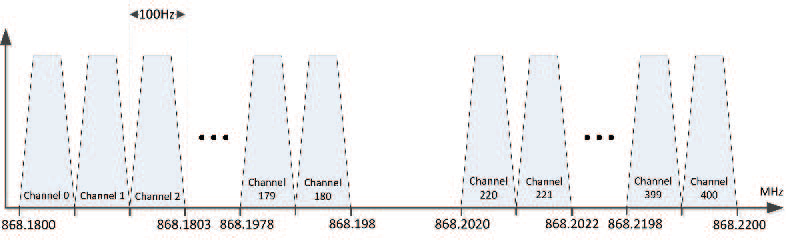
\includegraphics[scale=.5]{Immagini/DivisioneBande.png}

Fig. 4 I canali definiti 0 - 400 per 100 Hz nel range 868.180 - 868.220 MHz. % A
\end{figure}

\begin{figure}
\centering
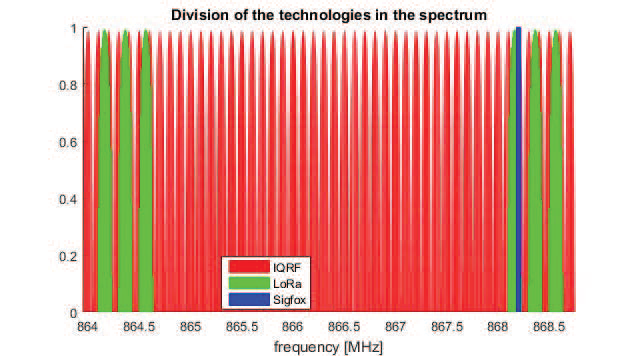
\includegraphics[scale=.5]{Immagini/DivB.png}

Fig. 5 Divisione delle tecnologie LoRa e Sigfox nell'intervallo 863,95 - 868,75 MHz. % B
\end{figure}

\begin{figure}
\centering
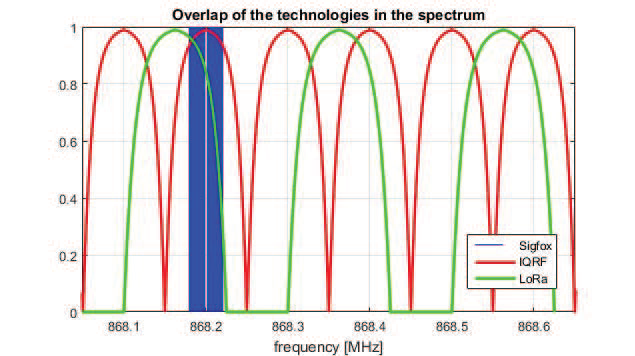
\includegraphics[scale=.5]{Immagini/DivisioneBande2.png}

Fig. 6 Divisione delle tecnologie nella gamma più piccola 868.05-868.65 MHz. % C
\end{figure}

\begin{figure}
\centering
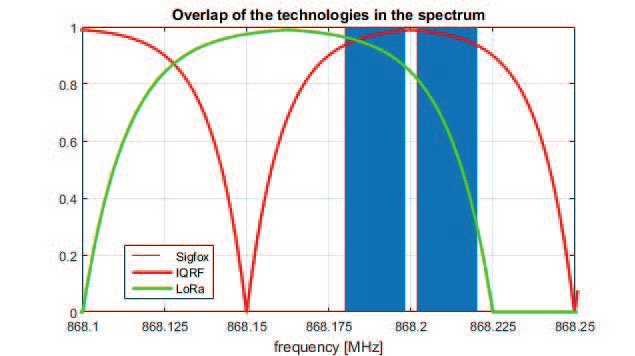
\includegraphics[scale=.5]{Immagini/DivB2.png}

Fig. 7 Divisione delle tecnologie nell'intervallo 868,1 - 868,25 MHz. % D
\end{figure}

\subsection{Copertura di LPWAN nello spettro}
Tutte le tecnologie LPWAN condividono e lavorano sulla stessa banda non licenziata. Non è scontato che queste tecnologie possano coesistere tutte contemporaneamente, senza sovrapporsi. Bisogna misurare con uno studio pratico le probabilità di collisione e la scabilità effettiva delle tecnologie. Nel caso in cui la coesistenza fosse positiva (quello che ci si aspetta) bisogna inoltre verificare che al crescere del numero di nodi finali per tecnologia i parametri di coesistenza nello spettro di frequenza restano costanti.
L'articolo \cite{art:rif.46} inizia descrivendo la distribuzione spettrale e i canali delle tecnologie LPWAN e SigFox. Esse sono mostrate in Fig. 4. I canali per downlink non vengono visualizzati in figura perché si trovano più in alto dei 869 MHz nello spettro e non si sovrappongono l'uno all'altro. La Figura 5 mostra solo i canali LoRa predefiniti più importanti per l'invio di messaggi JoinReq per connettersi alla rete. Tuttavia, LoRa può funzionare sui canali con quasi tutte le frequenze da 863 a 870 MHz. Sigfox copre davvero una piccola parte dello spettro. I canali di Sigfox assomigliano ad una sottile fascia in figura perché risulta piccola la loro larghezza di banda essendo di soli 100 Hz. 
La figura 6 mostra lo stesso spettro di frequenza ma con le tecnologie più in dettaglio. Questa parte dello spettro intorno a 868 MHz, vede coesistere tutte le tecnologie. LoRa ha 3 canali principali con larghezza di banda di 125 kHz che vengono utilizzati da ogni dispositivo LoRa. Sigfox ha localizzato tutti i canali attorno a 868,2 MHz. Lo spettro in un intervallo 868.10 - 868.25 MHz è illustrato in Fig. 7. Questa parte dello spettro contiene i canali principali, che hanno una grande importanza nel problema di potenziali collisioni e di coesistenza delle tecnologie. In questa fascia dello spettro che si sovrappongono le tecnologie LPWAN. Questa parte dello spettro, in particolare intorno a 868,2 MHz, potrebbe essere problematica, perché qui potrebbero verificarsi collisioni accidentali, che potrebbero interferire e interrompere la comunicazione (problema riscontrato anche nella verifica della mobilità in \cite{art:rif.47}). La probabilità di collisioni è molto più alta in questa fascia che in tutte le altre. La crescità prefista  di dispositivi che utilizzano queste tecnologie aumenta la possibilità di collisioni \cite{art:rif.46}.
Esistono molte altre tecnologie nel mondo, oltre a LPWAN, che vengono utilizzate per vari scopi e operano in molte bande di frequenza. Poiché l'intera banda di frequenza è un mezzo limitato e condiviso per tutti, è necessario tenere a mente anche queste tecnologie per una possibile coesistenza con LPWAN. Possibili complicazioni possono aumentare soprattutto nelle tecnologie che sono in conflitto di frequenza con le gamme di LPWAN. Per questo motivo vengono scelte le principali sei tecnologie che operano nelle frequenze simili come Personal Mobile Radio (PMR), trasmissione vocale wireless, reti mobili ecc... Le reti mobili LTE e GSM sono molto popolari e la divisione corretta di 800 o 900 MHz delle bande di frequenza secondo i documenti di definizione sono ben note. Coprono una grande quantità di frequenze nella banda di 800 MHz ad eccezione degli intervalli di sicurezza delle reti mobili. 
La prima tecnologia in conflitto nello spettro è utilizzata per i dispositivi di allarme, che utilizzano una comunicazione radio per un'indicazione di allarme che può verificarsi in un luogo lontano. La tecnologia ha specificato un piccolo ciclo di lavoro e un utilizzo molto ridotto dello spettro, che contribuisce a migliorare l'affidabilità. 
La seconda tecnologia per la trasmissione vocale wireless è definita per un apparecchio acustico, microfoni wireless, altoparlanti, cuffie e dispositivi per l'ascolto. La tecnologia RFID (Radio Frequency Identification) utilizza ricetrasmittenti radio e tag generalmente passivi. La tecnologia RFID è uno strumento per l'identificazione e il monitoraggio degli oggetti e per evitare furti, ecc... Queste due tecnologie non hanno definito il duty cycle (ciclo di lavoro o ciclo di lavoro utile, rappresenta la frazione di tempo che un'entità passa in uno stato attivo in proporzione al tempo totale considerato), poiché i dispositivi funzionano nella modalità Listen Before Talk (LBT). Anche queste tecnologie influenzeranno in qualche modo la coesistenza finale nella banda 863-870 MHz utilizzata dalle LPWAN. La barriera più grande potrebbero essere le reti mobili in base alla loro larghezza e al loro carattere, ma non si sovrappongono a LPWAN. È molto probabile che gli sviluppatori di LPWAN abbiano scelto proprio questa banda, a causa dell'assenza delle reti mobili. Altre tecnologie citate si sovrappongono già a LPWAN, ma non in modo pericoloso come le reti mobili perchè hanno un diverso carattere. Infatti, la tecnologia per dispositivi di allarme non crea un grosso rischio per la coesistenza utilizzando una parte sottile dello spettro e un piccolo ciclo di lavoro, sebbene i dispositivi di allarme utilizzino un intervallo di comunicazione globale. In caso contrario, la tecnologia di trasmissione vocale RFID e wireless hanno un raggio di comunicazione molto limitato. È possibile affermare che queste tecnologie si possono trovare solo in piccole aree durante i concerti o attorno a cancelli di sicurezza e si verificano occasionalmente. Ciò minimizza rapidamente le possibilità di potenziali problemi con le tecnologie operative parallele \cite{art:rif.46}.

\subsubsection{Probabilità di occorrenza sul canale}
Tutti i calcoli e le considerazioni sulla distribuzione del tempo e sulla probabilità delle tecnologie Lora, Sigfox e IQRF (altra tecnologia LPWAN che condivide la stessa banda) sono fatti assumendo che tutte le tecnologie stiano lavorando su canali di frequenza di sovrapposizione. È solo una singola combinazione possibile di canali per queste tecnologie, Fig. 5. Include il canale LoRa che inizia a 868.1 MHz, il canale IQRF n. 50 a partire da 868.15 MHz e tutti i canali Sigfox grazie alla sua larghezza di banda \cite{art:rif.46}. 
Questi canali sono mostrati in dettaglio in Fig. 7. È possibile considerare la tempistica delle singole tecnologie e le loro risultanti statistiche e probabilità, che suggeriscono una possibile coesistenza reciproca sullo stesso canale. Le varianti individuali con il tempo di caricamento maggiore sul canale, quindi in termini di tempo è la peggiore opzione possibile, vengono selezionate per il calcolo della probabilità risultante. La tecnologia Sigfox offre solo una variante \cite{art:rif.46}.
\begin{center}
\begin{tabular}{r|c|c|c|}
&LoRa DR0&Sigfox&IQRF low DR\\ \hline
Bit rate [bit/s]&250&100&1200\\ \hline
Max payload [B]&59&12&64\\ \hline
Periodo di trasmissione [s]&2.30&2.00&0.85\\ \hline
$E_1$ [s]&378.28&840.00&119.47\\ \hline
$E_2$[\%]&0.4378&0.9722&0.1383\\ \hline
$P_E$ [-]&0.004378&0.009722&0.001383\\ \hline
\end{tabular}
Tabella 1. \\
$E_1$ = evento sul canale durante un 24 ore. \\
$E_2$ = evento sul canale durante un 24 ore. \\
$P_E$ = Probabilità dell'evento sul canale. \\
I dati raccolti appartengono agli autori dell'articolo \cite{art:rif.46}. \\

\end{center}
La tabella 1 mostra il confronto e dati di queste tre tecnologie. Un periodo di trasmissione viene calcolato dalla velocità dati e dalla dimensione del messaggio. Lo strumento Lora Modem Calculator è stato utilizzato per i dispositivi LoRa. Viene inoltre menzionato il tempo di occorrenza per ciascuna delle varianti durante 24 ore per un confronto migliore. Un prerequisito per tutte le tecnologie è stato una trasmissione di 140 messaggi al giorno, ovvero il valore massimo definito per la tecnologia SigFox. Una parte di quel tempo è anche un periodo di messaggi di ritrasmissione che si verificano nei dispositivi SigFox e tempi di trasmissione per il downlink, che sono definiti in modo diverso per ciascuna tecnologia. Secondo il carico di tempo parametrico precedentemente menzionato, la variazione Sigfox è con un bit rate di 100 bit/s e massimo carico utile di 12 B nel caso peggiore. Questo è principalmente dovuto al fatto che SigFox invia ogni messaggio tre volte. Sono trasmessi su frequenze diverse, ma la loro posizione interferisce ancora con la zona problematica menzionata. LoRa DR0 e IQRF low DataRate risparmiano più tempo. Le ragioni di una così grande differenza sono date dalla struttura della tecnologia, che utilizza le tecniche UNB, larghezza di banda ridotta, bassa velocità in bit e un piccolo volume di dati. SigFox ha quindi scelto altre priorità nella sua politica, come la lunga autonomia e una maggiore durata della batteria a scapito della velocità o della sicurezza contro gli errori di trasmissione \cite{art:rif.46}.

\subsubsection{Probabilità di collisione sul canale}
La probabilità che si verifichi una collisione in un canale multiplo è una questione cruciale per la coesistenza delle diverse tecnologie viste nell'articolo \cite{art:rif.46}. Il tutto è considerato e calcolato con le varianti nel caso peggiore possibile, così da valutare il potenziale possibile di coesistenza per le tecnologie citate. La quantità approssimativa di equipaggiamento di ciascuna tecnologia è stata stimata in modo che la probabilità di collisione sia adeguata per il corretto funzionamento di tutti i processi, e per farlo bisognava verificare la quantità di tempo che ciascuna tecnologia trascorre sul canale. Questi valori sono stati misurati e riportati dagli autori nella tabella 1. La probabilità di collisione durante un giorno (24 ore) è basata sul rapporto tra il tempo in cui la tecnologia utilizza il canale e il tempo totale. La probabilità che avvenga l'evento è il principale valore che può essere confrontato con gli altri o utilizzato per calcolare la probabilità di collisioni. Le specifiche dell'autorizzazione generale numero VO-R / 10 / 05.2014-3  definisce che il duty cycle massimo ammissibile è determinato dalla percentuale di tempo in cui il dispositivo può essere attivo sul canale. Tutte le tecnologie citate soddisfano questa condizione, sebbene SigFox con rapporto 0,009722 si adatti al limite 0,01 solo con un piccolo margine. La probabilità calcolata di collisione descrive una situazione in cui due o più dispositivi diversi sul canale si scontrano allo stesso tempo. Dai risultati in tabella 1 viene evidenziato che la probabilità che due o più dispositivi diversi sul canale si scontrano allo stesso tempo è molto bassa e quindi molto inferiore alla probabilità dell'evento delle singole tecnologie. La probabilità aumenterà significativamente con il numero crescente di dispositivi e il limite sarà inevitabilmente vicino 1, evento di probabilità certa \cite{art:rif.46}.
% Calcolo della probabilità di collisione: %
I problemi di coesistenza di tecnologie per un numero maggiore di dispositivi sono molto importanti per determinare i limiti della tecnologia. Il limite della quantità di dispositivi non deve essere superato per evitare il deterioramento della qualità o della disponibilità di servizi in esecuzione su queste tecnologie. I problemi relativi al calcolo della probabilità di collisione per un numero maggiore di dispositivi di ciascuna di queste tecnologie sono notevolmente complicati. Gli stati problematici di collisione sono definiti per due o più dispositivi attivi simultaneamente. % Troppo difficile? Si può omettere? %
La complessità del calcolo aumenta per via delle variabili da considerare, perché il numero degli stati probabilistici aumenta con il numero di $n$ dispositivi in base a:
\begin{equation}
S = 3n + 1
\end{equation}
dove $S$ è il numero di stati probabilistici e $n$ è il numero di dispositivi di ciascuna tecnologia. Il calcolo della probabilità di collisione in caso di un numero maggiore di dispositivi che utilizzano ciascuna tecnologia è definito come:
\begin{equation}
P(N \leq n) = 1 - n(P_L + P_S + P_I) - P'_0
\end{equation}
dove ogni parametro descrive stati specifici di probabilità come descritto di seguito. Tutte le variabili sono state calcolate dai valori già noti di probabilità degli eventi in tabella 1. Qui viene usato il complemento per esprimere l'evento opposto, che è etichettato come $c$ in apice. Un prerequisito è che il numero di dispositivi $n$ sia lo stesso per tutte le tecnologie.
\begin{equation}
P_L = P(L)P(L^c)^{n-1}P(S^c)^nP(I^c)^n
\end{equation}
\begin{equation}
P_S = P(L^c)^nP(S)P(S^c)^{n-1}P(I^c)^n
\end{equation}
\begin{equation}
P_I = P(L^c)^nP(S^c)^nP(I^c)^{n-1}
\end{equation}
\begin{equation}
P'_0 = (P(L^c)P(S^c)P(I^c))^n
\end{equation}
dove $N$ è il numero di dispositivi di ciascuna tecnologia durante la collisione. La risultante dipendenza della probabilità di collisione su un canale è presente dopo la sostituzione nell'equazione (2.2) altrimenti troppo lunga e difficile da comprendere, quindi è divisa in sottosezioni, che illustrano chiaramente il loro utilizzo. % I risultati del calcolo della probabilità di collisione per il numero crescente di dispositivi. Funzione di distribuzione del numero di dispositivi %
\begin{figure}
\centering
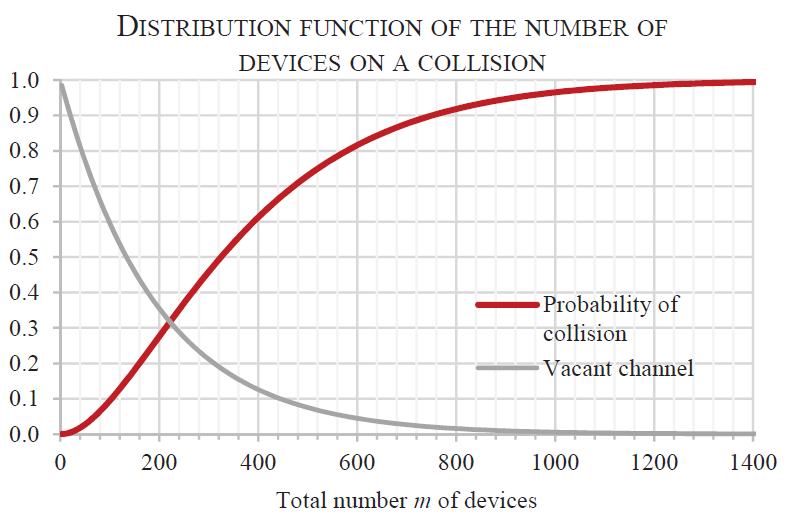
\includegraphics[scale=.5]{Immagini/DistribuzioneDiProb.png}

Fig. 8 Distribuzione della funzione di probabilità di collisione 2 o più dispositivi.
\end{figure}

La funzione di distribuzione mostrata in figura è basata su (2.2). Dipende dall'aumento del numero totale $m$ dei dispositivi, che è il numero n dei dispositivi di ciascuna delle tre tecnologie (2.3), (2.4) e (2.5).
\begin{equation}
m = 3n 
\end{equation}
\begin{equation}
F(m) = 1 - (P_L+P_S+P_I)m/3 - P'_0 
\end{equation}
Essa non è una funzione lineare del processo come potrebbe sembrare la soluzione più semplice per il crescente numero di dispositivi come nel grafico in figura. Tuttavia, può essere approssimata da una curva polinomiale almeno al $4^{\circ}$ ordine. La funzione inizia da zero ed è ad uno nel limite, che è un limite previsto dalla natura del calcolo. il grafico mostra anche la curva di probabilità del canale non occupato, che è inizialmente quella dovuta all'assenza di qualsiasi dispositivo sul canale. Il decorso della curva decade in modo esponenziale con il quadrato del numero $n$ di dispositivi di ciascuna tecnologia. Questo corso è calcolato da:
\begin{equation}
P'_0 = (P(L^c)P(S^c)P(I^c))^n 
\end{equation}
\cite{art:rif.46}
% Omettere fino a qui %

\subsubsection{Capacità del numero di dispositivi sul canale}
La questione della coesistenza dipende da due fattori principali, che hanno i loro limiti, vale a dire la \textbf{distribuzione di frequenza} e \textbf{la distribuzione temporale}. La divisione del tempo è composta principalmente dalla probabilità di occorrenza delle singole tecnologie e quindi dalla probabilità di collisioni sul canale. Dai risultati  dell'esperimento \cite{art:rif.46} si può ipotizzare ulteriori limiti in questi sistemi di trasmissione. Uno dei limiti principali è la potenziale capacità massima del numero di dispositivi che operano sul canale. Si basa sull'utilizzo del canale, cioè quanto gravano i dispositivi. In altre parole, esprime i confini, in cui è possibile far funzionare il sistema senza perdere qualità o far diminuire la disponibilità dei servizi gestiti. Alcuni parametri che determinano la qualità dei servizi sono detti Quality of Service (QoS) e Quality of Experience (QoE). Il numero dei dispositivi sul canale è una questione vitale per la crescita delle tecnologie. Devono dimensionare la propria rete in conformità con la capacità massima prestabilita di un canale rispetto ad altre possibili tecnologie sulle stesse frequenze. Inoltre, spesso devono rispettare la disponibilità del servizio pianificata in base al documento SLA (Accordo sul livello di servizio), che è organizzato e tracciato tra il fornitore del servizio e l'utente. Il dimensionamento accurato del numero di dispositivi sul canale non è del tutto possibile. Dipende da molti fattori che descrivono lo stato del canale, la qualità, la disponibilità dei servizi usati e la probabilità di collisione con più dispositivi. Quest'ultimo pararamentro il termine che descrive il vero stato del canale con un certo numero di dispositivi collegati. Dal grafico in figura 8 è stato possibile stimare approssimativamente quale potrebbe essere la capacità massima del canale. Dipende anche da altri parametri dei singoli servizi operativi come la disponibilità del servizio e una modalità di implementazione dei parametri QoS e QoE per riservare e gestire i flussi di dati. I parametri QoS e QoE sono indicatori di un livello di qualità e quindi solo i loro protocolli reagirebbero se le condizioni si deteriorassero a causa, ad esempio, di un numero maggiore di dispositivi sul canale rispetto alla capacità massima determinata. Pertanto, è importante per l'ideale e il corretto funzionamento dell'intera rete, non deve superare la capacità massima del canale. È persino difficile trovare il limite senza prove sperimentali sul canale con tecnologie e servizi concreti \cite{art:rif.46}.
% L'occorrenza sul canale durante un giorno di tecnologia Sigfox è più del doppio rispetto a LoRa e oltre sette volte superiore alla tecnologia IQRF. È causato da una diversa scelta in termini di politica, ad esempio autonomia e durata della batteria, a scapito della velocità o della sicurezza degli errori di trasmissione. %
Dai risultati calcolati nell'articolo \cite{art:rif.46} la probabilità di occorrenza dei dispositivi sul canale durante un giorno, è possibile confermare che tutte le tecnologie soddisfano le condizioni del ciclo di lavoro massimo consentito. La funzione di distribuzione della probabilità di collisione due o più dispositivi tende ad 1 per più di 1000 dispositivi attivi simultaneamente. Oggigiorno c'è ancora una piccola parte dei dispositivi attivi costruiti sulla base delle tecnologie LPWAN. Dovrebbe evolversi in un prossimo futuro, perché LoRa e Sigfox promettono un grande sviluppo e più di migliaia di dispositivi posizionati. Quindi il problema della coesistenza della tecnologia LPWAN diventa più che reale \cite{art:rif.46}.

\subsection{Protocollo LoRa / Lv 1}
LoRa è l'acronimo di Long Range, lungo raggio, che sta a riassumere il vantaggio principale di questa tecnologia wireless, senza cablature riesce a connettere lunghe distante. LoRa è una modulazione radio a spettro esteso brevettata (EP2763321 dal 2013 e US7791415 del 2008) sviluppata da Cycleo (Grenoble, Francia) e acquisita da Semtech NASDAQ: SMTC nel 2012 \cite{art:rif.30}. 
LoRa è basata sulla tecnica CSS (Chirp Spread Spectrum), che la rende in grado di variare la lunghezza del cosiddetto fattore di spreading (compreso tra 6 e 12 bit) e l'ampiezza di banda in funzione della bit rate (ovvero il numero di bit trasmessi al secondo) richiesta nel range compreso tra 20bit/s a 41kbit/s \cite{art:rif.23}. 
Questa modulazione aumenta la tolleranza alla deviazione di frequenza, riducendo i costi. Inoltre rende LoRa una buona resistenza contro lo sbiadimento del multipath e l'effetto Doppler, e migliora la sensibilità del ricevitore aumentando la copertura \cite{art:rif.44}. 
Grazie alla straordinaria modulazione del chirp, il collegamento wireless può raggiungere una sensibilità fino a -137 dBm e fino a 157 dB di budget di collegamento. Il trade-off è la velocità dati raggiungibile, che è nell'intervallo di kilobit al secondo. Questo paramentro permette di capire che è una tecnologia adatta per servire l'Internet of Things (IoT) e le applicazioni M2M, mentre non è assolutamente adatta, per esempio, allo streaming video. LoRa può essere utilizzato su un'ampia gamma di frequenze da 137 MHz a 1020 MHz. Questo include numerose bande ISM prive di licenza come 169 MHz, 433 MHz, 868 MHz e 915 MHz. Questo è un fattore chiave per implementazioni e interoperabilità a livello mondiale \cite{art:rif.30}. 
La rivista di settore \cite{art:rif.23} descrive Lora come "Tecnologia realmente innovativa che fissa un nuovo punto di riferimento in termini di distanza di trasmissione e di consumi di potenza, la tecnologia LoRa adotta uno schema di modulazione digitale completamente asincrono. La modulazione garantisce una continuità di fase tra i simboli chirp nella parte del preambolo del pacchetto. Questa funzione consente di utilizzare la sincronizzazione temporale più semplice e quindi componenti meno costosi. Una radio LoRa ha quattro parametri di configurazione: frequenza portante, fattore di diffusione (SF, spread factor), larghezza di banda e velocità di codifica. La selezione di questi parametri determina il consumo di energia, il raggio di trasmissione e la resilienza al rumore. A differenza di SigFox, la tecnologia LoRa può essere utilizzata in reti sia private sia pubbliche. Le elevate prestazioni che la tecnologia LoRA è in grado di offrire sono testimoniate dalla sua capacità di ricevere segnali fino a -22dB al di sotto della soglia del rumore di fondo, abbinata alla reiezioni dei canali adiacenti di almeno 69dB con un offset di 25kHz, un valore migliore di 30dB rispetto a quello che si ottiene utilizzando la modulazione FSK a 868MHz sui medesimi transceiver. Un tempo le radio in banda ISM destinate ad applicazioni industriali e operanti a frequenze inferiori a 1GHz erano caratterizzate da un range in campo aperto limitato a 2 km" \cite{art:rif.23}. 
% LoRa è lo strato fisico della pila ISO/OSI. 
Nonostante condividano la stessa banda, LoRa si distingue da SigFox, per la capacità di gestire segnali più deboli al costo di leggero consumo di energia, che resta comunque basso da rientrare nelle LPWAN, in in confronto a 2G, 3G, ecc... a parità di distanza raggiunta.

L'articolo \cite{art:rif.48} descrive come una configurazione di modulazione (data-rate, DR) è data da due parametri: una larghezza di banda (BW, bandwidth) e un fattore di diffusione (SF, spread factor) specificati dalla specifica dei parametri regionali LoRaWAN. Le larghezze di banda vanno da 125 kHz a 500 kHz a seconda della regione. La durata del simbolo chirp è data da:
\begin{equation}
 T_s = \frac{2^{SF}}{BW}
\end{equation}
dove SF appartiene all'intervallo [7, 12]. Il TOA (time-on-air) dipende quindi in modo esponenziale dalla SF. D'altra parte la sensibilità del ricevitore è proporzionale alla SF. Inoltre, la tecnica dello spettro esteso è combinata con la correzione degli errori in avanti (FEC, forward error correction) con velocità di codifica in {4/5; 4/6; 4/7; 4/8}. Un pacchetto LoRa costituito da un preambolo, un'intestazione, un payload e un campo CRC \cite{art:rif.48}. 
Il preambolo permette al ricevitore, solitamente un Gateway LoRa, di sincronizzarsi con il messaggio in arrivo. Nell'intestazione ci sono tutte le informazioni per notificare delle informazioni al trasmettitore. 
LoRa implementa la modulazione wireless utilizzata per creare il collegamento di comunicazione a lungo raggio. 
Il suo schema di modulazione a largo spettro consente un'operatività a lungo raggio e un'elevata capacità di rete, con bassa potenza a radiofrequenza. Grazie alla richiesta energetica contenuta, l'end-point di una rete LoRa con alimentazione a batteria può funzionare per molti anni, una durata sufficiente in molte applicazioni, che ha un sensibile effetto sui costi operativi di una rete con numerosi end-point \cite{art:rif.23}. 
Per favorire l'inizio degli sviluppi basati sulla tecnologia LoRa, esiste un portafoglio di moduli radio conformi alle specifiche LoRaWan per consentire di semplificare e accelerare l'integrazione di questa tecnologia nei dispositivi IoT. I moduli Microchip, come l'RN2483, sono dispositivi plug-and-play che integrano un completo sottosistema radio con un microcontrollore, le Eeprom di identità, il front-end a radiofrequenza e i relativi circuiti, oltre a un cristallo. Questi moduli sono fra i primi che hanno passato il collaudo LoRa Alliance Certification \cite{art:rif.20}. 
La soluzione LoRa può essere etichettata come CDMA. Sta usando diversi fattori di diffusione (velocità dati chirp) e velocità di codifica per segnali multiplex su una singola frequenza. Ciò non solo aumenta la capacità della rete, ma consente anche l'adattamento dinamico delle velocità dei dati del dispositivo. I dispositivi con un migliore collegamento a un gateway (a causa della vicinanza, di un ambiente a bassa rumorosità, di una visuale non ostruita) possono utilizzare velocità di trasmissione dati superiori (fino a 11 kbps) e risparmiare batteria. I dispositivi con una scarsa qualità dei collegamenti possono aumentare il budget dei collegamenti utilizzando velocità di trasmissione inferiori, estendendo il raggio di collegamento effettivo a oltre 30 km in linea di vista \cite{art:rif.30}. 
LoRa è tecnologia particolarmente adatta per sistemi di controllo e di misurazione su territori vasti vantando la minima spesa rispetto alle tecnologie concorrenti, al costo di una trasmissione più lenta delle informazioni. Questo non deve essere visto come uno svantaggio, perchè permette al livello fisico di ottenere delle ottimizzazioni sull'accesso multiplo al canale in caso di rilevamento di collisioni, a differenza delle altre tecnologie concorrenti.

\subsubsection{Tempo di trasmissione on-the-air}
Nell'articolo \cite{art:rif.44} LoRa è stata messa alla prova a differenti combinazioni di fattori metereologici per analizzare i limiti di questa tecnologia in un ambiente urbano per capire, in questo modo si può capire fino a dove ci si può spingere nella creazione di Smart City. Secondo "LoRa Modem Designer’s Guide" della Semtech e come menzionato precedentemente, il pacchetto LoRa è costituito da un preambolo e da payload (che a sua volta può contentere un intestazione). Il tempo di trasmissione in onda è la somma del preambolo e della durata del carico utile. Il tempo di trasmissione in diretta ToA è indicato:
\begin{equation}
T_{oA} = T_{preamble} + T_{payload} = \\
\end{equation}
\begin{equation}
= T_{sym}(L_{preabmle}+L_{payload}) = \\
\end{equation}
\begin{equation}
= \frac{2^{SF}}{BW}\times((n_{preamble}+4.25)+(8+max(ceil(\frac{8PL-4SF+42-20H}{4(SF-2DE)}\times(CR+4),0))))
\end{equation}
Dove la larghezza di banda BW assume valori in {62,5 kHz, 125 kHz, 250 kHz, 500 kHz }, SF è il fattore di diffusione, $T_{sym}$ è il tempo di trasmissione del simbolo, determinato da SF e BW, $n_{preamble}$ è la lunghezza del preambolo programmato, PL è il numero di byte del carico utile, H = 0 significa presenza dell'intestazione, H = 1 quando non è presente un'intestazione, DE = 1 vuol dire che è stata impostata l'ottimizzazione a bassa velocità di trasmissione dati, altrimenti DE = 0, CR varia da 1 a 4 (corrispondente alla velocità di codifica da 4/5 a 4/8). Secondo la formula, il tempo di trasmissione in onda è inversamente proporzionale a BW e aumenta con l'aumento di SF. Sono stati fatti esperimenti per verificare la relazione tra tempo di trasmissione on-air, SF e BW, e confermano quanto predetto in teoria \cite{art:rif.44}.
Grazie a questo studio possiamo intuire un problema legato all'aumento dei dispositivi LoRa e LPWAN. La banda va distribuita tra i vari dispositivi LoRa e tecnologie LPWAN concorrenti. Se la banda assegnata ad un dispositivo scarseggia, per trasmettere una certa quantità di informazione ad una certa frequenza (limitata nelle specifiche LoRa), sarà necessario più tempo per consegnare l'informazione. All'interno di questa quantità di tempo c'è una maggiore probabilità che il segnale possa interrompersi e peggiorare le prestazioni del sistema. 

\subsubsection{Copertura del segnale}
I moduli funzionavano in banda di frequenza 433 MHz con potenza di trasmissione di 100 mW e guadagno dell'antenna di 6 dBi. Gli autori dell'articolo \cite{art:rif.44} hanno effettuato le misurazione riportati nella tabella 2. I risultati mostrano la distanza più lontana raggiunta mantenendo la perdita dei pacchetti inferiore al 10\%, con SF e BW diversi. Questo dimostra che l'aumento dell'intervallo dipende dalla diminuzione di BW o dall'aumento di SF, poiché BW più piccoli e SF più grande possono migliorare significativamente la sensibilità. Tuttavia è necessario tenere conto, oltre all'ampia copertura e al basso consumo energetico, della velocità di trasmissione e del ritardo di trasmissione. In questo sperimento SF di 7 e BW di 125 kHz rappresentano il compromesso ottimale \cite{art:rif.44}.
Per quanto possa essere discutibile la scelta la solia della perdita dei pacchetti fissata al 10\%, la disponibilità di banda è il fattore principale che permette di raggiungere lunghe distanze con una pardita di pacchetti accettabile. Le lunghe distanze promesse in fase teorica devono fare i conti con le condizioni climatiche che affliggono il territorio.

\begin{center}
\begin{tabular}{r|c|c|}
SF&BW (kHz)&Portata inferiore al 10\% della perdita di pacchetti (m)\\ \hline
7&250&2910-3110\\ \hline
9&250&3140-3340\\ \hline
9&500&2130-2330\\ \hline
11&500&4810-5010\\ \hline
\end{tabular}
Tabella 2. \\
Le misurazioni sono state raccolte dagli autori dell'articolo \cite{art:rif.44}. \\
\end{center}

\subsubsection{LoRa PHY error model}
L'articolo \cite{art:rif.49} descrive nel dettaglio i livelli e i sottolivelli della pila di protocolli della tecnologia LoRa.
\begin{enumerate}
\item Implementazione della banda base LoRa PHY: 
"per modellare gli effetti della perdita del percorso e dell'interferenza intra-LoRa, è stato sviluppato un modello di errore per LoRa PHY. È stato misurato il bit error rate (BER) per diverse configurazioni LoRa PHY su un canale AWGN (Additive White Gaussian Noise, rumore gaussiano bianco additivo). Un diagramma a blocchi delle simulazioni BER è mostrato in figura 7. I bit di informazione generati nella sorgente di informazioni sono mappati ai bit di codice dall'encoder di correzione dell'errore. Questo codificatore implementa le code rate 5/4, 7/4 e 8/4 disponibili in LoRa.1, mentre il 5/4 CR è un semplice codice di controllo di parità, i CR 7/4 e 8/4 sono (7, 4) e (8, 4) codici di Hamming che correggono gli errori lineari. Questi codici possono correggere un errore di un bit e rilevare fino a due errori di bit. Successivamente, l'interleaver diagonale mischia i bit di codice in modo tale che alla sua uscita, i gruppi di bit PPM siano costituiti da bit della stessa posizione di bit di parole di codice consecutive PPM. Ad esempio, la prima parola di uscita raggruppa i bit in posizione 0 da parole in codice consecutivo PPM. PPM rappresenta la lunghezza di bit delle parole di uscita dell'interleaver. In LoRa il PPM di theinterleaver è uguale a LoRa SF. Di conseguenza, il numero di bit mappati per il simbolo LoRa è uguale a SF. A causa dell'interlacciamento, un simbolo perso nel ricevitore viene convertito in errori PPM a 1 bit su parole di codice consecutive PPM (piuttosto che un errore di bit PPM in una parola di codice senza interleaver). Dopo l'interleaver, le parole di output vengono sbiancate per aumentare l'entropia della fonte di informazioni. Si noti che nelle simulazioni BER i bit di informazione sono tratti da una distribuzione uniforme, pertanto l'entropia della fonte di informazioni è già al massimo. Prima di passare il flusso di bit sbiancato al modulatore, è prima mappato in grigio inverso. Questo produce una sequenza di numeri interi, che vengono inviati al modulatore LoRa. Al modulatore LoRa, una sequenza di campioni $N$ complessi di time-shifted in banda base risulterà generata tramite un accumulatore di fase come indicato dal sistema (2.12), dove $N$, il numero di campioni per simbolo di banda base, è uguale a $2^{SF} (f_s / BW)$. Il numero intero di input determina il time-shift del up-chirp:
\begin{equation}
m(i) = \bigg \{
\begin{array}{rl}
exp(-j\pi) & (i = 0)\\
m(i-1)exp(if(i)) & (i = 1, \dots, N-1)\\
\end{array}
\end{equation}
dove la frequenza istantanea f (i) è data da:
\begin{equation}
f(i) = -\pi + {i \over N} 2\pi  
\end{equation}
per i = 1, /dots, N-1. Successivamente, i campioni del simbolo LoRa vengono inviati sul canale AWGN per un determinato rapporto tra segnale e rumore (SNR) come da:
\begin{equation}
c(i) = m(i) + \sqrt{E_s \over 2SNR}[N(0; 1) + jN(0; 1)]
\end{equation}
per i = 0, \dots, N-1. Dove N(0; 1) è la distribuzione normale standard e $SNR = 10^{SNR_{dB} / 10}$. Si noti che l'energia per simbolo è uguale a quella del modulatore LoRa.
Al ricevitore, il demodulatore LoRa utilizza una demodulazione basata sulla correlazione in cui il simbolo ricevuto è correlato a tutti i simboli LoRa noti. La decisione su quale simbolo è stato inviato, viene effettuata selezionando il simbolo LoRa con il valore di correlazione massimo. Dopo la demodulazione, la catena di ricezione è l'opposto della catena di invio. Il tasso di errore viene misurato nei bit di informazione, dopo la correzione dell'errore \cite{art:rif.49}.

\begin{figure}
\centering
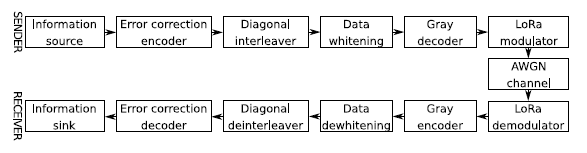
\includegraphics[scale=.7]{Immagini/SchemaABlocchi.png}

Fig. 9 Schema a blocchi dell'implementazione della baseband LoRa PHY: mittente, canale AWGN e ricevitore.
\end{figure}
\item LoRa PHY BER Simulazioni:  
Al fine di determinare il BER dello strato fisico LoRa, sono state eseguite simulazioni per i parametri LoRa PHY elencati in Tabella 3. 
\begin{center}

\begin{tabular}{|c|c|c|c}
BW (kHz)&SF&CR&SNR(dB)\\ \hline
125&7&1,3&[-20,0]\\ \hline
125&8&1,3&[-20,0]\\ \hline
125&9&1,3&[-20,-8]\\ \hline
125&10&1,3&[-20,-8]\\ \hline
125&11&1&[-23,-13]\\ \hline
125&11&3&[-25,-13]\\ \hline
125&12&1,3&[-26,-17]\\ \hline
\end{tabular}
Tabella 3, parametri LoRa PHY per simulazioni BER. \\
Le misurazioni sono state effettuate dagli autori dell'articolo \cite{art:rif.49}. \\
\end{center}
Non è stato eseguito il sovracampionamento, pertanto continua a valere $N = 2^{SF}$. Le simulazioni sono state eseguite per valori SNR in passi di 1 dB negli intervalli come pubblicati nella tabella 3.
Successivamente, una curva esponenziale come definita dall'equazione (2.15) è stata adattata a un sottoinsieme dei valori logaritmici dei valori BER misurati.
\begin{equation}
log_{10}(BER (SNR_{dB})) = \alpha exp (\beta SNR_{dB})
\end{equation}
Il sottoinsieme dei valori BER utilizzati per l'adattamento della curva è stato determinato come segue. Innanzitutto, i valori BER misurati pari a zero sono stati scartati. In secondo luogo, i valori BER sono stati aggiunti al sottoinsieme fino a quando il BER ha raggiunto un valore in cui la velocità di consegna del pacchetto (PDR) corrispondente è scesa sotto uno su un milione per un pacchetto di 13B. La lunghezza del pacchetto di 13B deriva dalla lunghezza minima del payload LoRa PHY per una trasmissione LoRaWAN: 1B intestazione MAC, intestazione frame 8B e 4B MIC (Message Integrity Code). Inoltre, per ogni curva si è scelto un punto di taglio SNR in modo che il PDR per un pacchetto 13B (= 108b) fosse uguale a uno su un milione nel punto limite.  
\end{enumerate}
Si noti che i PDR presentati tengono conto di tutti i pacchetti generati, anche i pacchetti che sono in coda per la trasmissione vengono conteggiati verso PDR. Pertanto, il PDR riflette il throughput di rete complessivo (per lo stesso numero di dispositivi e periodo di dati)" \cite{art:rif.49}.
La tecnologia LoRa in letteratura viene associata al modello della tecnologia ALOHA. Questa associazione è utile per utilizzare modelli funzionati e collaudati per misurare le prestazioni di tecnologie simili e metterle a confronto. Questo approccio però non tiene contro della diversità dei due protocolli. ALOHA quando percepisce una collisione scarta i pacchetti letti e notifica secondo gli standard del protocollo l'avvenuta collisione. LoRa PHY quando percepisce una collisione finisce la lettura del pacchetto e procede con la controllo degli errori. Questa scelta è dovuta alla particolare modulazione di LoRa che è meno sensibile agli errori in ricezione. Pertanto i pacchetti considerati scartati dai classici modelli ALOHA in realtà vengono letti correttamente, per questo LoRa PHY error model da una stima più accurata delle prestazioni LoRa.    

\subsubsection{Assegnazione dei fattori di diffusione}
Il primo problema che è stato studiato è come assegnare LoRa SF per i dispositivi terminali. Le SF hanno un forte impatto sui PDR. La sottostima della SF (ad esempio, l'assegnazione di una SF, cioè troppo bassa) può causare errori di ricezione a causa del basso SNR. Sovrastimare la SF (ad esempio, assegnare una SF, cioè troppo alta) può portare a un uso inefficiente del tempo di propagazione aerea. Sono state prese in considerazione tre strategie di assegnazione di SF.
\begin{enumerate}
\item Random: assegna le SF ai dispositivi terminali secondo una distribuzione casuale uniforme.
\item Fixed: assegna lo stesso SF ai dispositivi terminali.
\item PER: per ogni dispositivo finale, trova e assegna il valore SF più basso per il quale il tasso di errore del pacchetto scende al di sotto di una determinata soglia.
\end{enumerate}
I pacchetti vengono inviati come messaggi non confermati. La strategia PER possiede il miglior PDR. I PDR per le diverse soglie di PER sono molto simili e non esiste una soglia che produca il PDR più alto in tutte le dimensioni di rete considerate. Si noti che per reti di piccole dimensioni (vale a dire, meno di 100 dispositivi finali) il PDR al 75\% della strategia fissa SF12 potrebbe essere sufficiente. Poiché ciò elimina la necessità di velocità di trasmissione dati attiva (ADR) in reti così piccole, il traffico downstream di ADR può essere evitato. Ovviamente l'invio a una velocità dati inutilmente elevata fa sì che un dispositivo finale sprechi energia. Con l'aumentare del numero di dispositivi (vale a dire più di 1000 dispositivi finali), la strategia casuale supera le strategie fisse in termini di PDR. Ciò è spiegato dal fatto che per le reti di maggiori dimensioni le perdite sono dovute principalmente alle collisioni e che la strategia casuale riduce il numero di collisioni (rispetto a una strategia fissa) sfruttando l'ortogonalità dei diversi SF \cite{art:rif.49}.

\subsection{Protocollo LPWAN / Lv 2}
LoRaWAN (Low-power Wide area network) è una specifica del protocollo costruita sulla tecnologia LoRa sviluppata dalla LoRa Alliance. Utilizza lo spettro radio senza licenza nelle bande Industrial, Scientific e Medical (ISM) per consentire la comunicazione a bassa potenza ed ampia area tra i sensori remoti e i gateway collegati alla rete. LoRaWAN è il protocollo MAC per la rete di nodi LoRa ad alta capacità. È uno standard LPWAN aperto gestito dalla LoRa Alliance. Sfrutta le funzionalità LoRa appena descritte ed ottimizza la durata della batteria e la qualità del servizio per i nodi LoRa. Questo approccio basato su standard per la creazione di una LPWAN consente di configurare rapidamente reti IoT pubbliche o private ovunque utilizzando hardware e software che sia bidirezionale, sicuro, interoperabile e mobile, fornisca una localizzazione accurata e funzioni come previsto \cite{art:rif.24}. 
LpWan su LoRa(tecnologia sub-GHz a basso consumo) supporta una velocità dei dati da 0,3 kbps a 50 kbps, in funzione della distanza e della durata dei messaggi. La distanza di trasmissione può raggiungere 15 - 20 km. Anche in un ambiente urbano ad alta densità si possono coprire distanze di comunicazione di oltre 2 km \cite{art:rif.20}. 
Il protocollo è completamente bidirezionale, che consente una consegna affidabile dei messaggi (conferme). Comprende la definizione della crittografia end-to-end per la sicurezza e la riservatezza dei dati, la registrazione over-the-air dei nodi finali e la funzionalità multicast. Grazie al modello di antenna distribuita e ai gateway GPS abilitati, la rete è in grado di localizzare la posizione dei nodi, anche quando sono mobili \cite{art:rif.30}.
I sensori LoRaWAN sono in grado di comunicare a distanze superiori ai 100 km (62 miglia) in ambienti favorevoli, 15 km (9 miglia) in ambienti semi-rurali e a più di 2 km (1,2 miglia) in ambienti urbani densamente popolati ad una velocità di dati da 300 bit a 100 kbit. Questo li rende adatti all'invio di quantità di dati contenute, come le coordinate GPS e le letture del clima che la banda larga non è in grado di raggiungere. I sensori richiedono inoltre pochissima energia, la maggior parte di loro può funzionare per più di 10 anni con una sola batteria AA e, inoltre, le chiavi AES128 rendono praticamente impossibile l'intercettazione e la manomissione delle comunicazioni \cite{art:rif.25}. 
In pratica è altamente efficiente dal punto di vista energetico ed economico: l'industria ha come target la durata della batteria di oltre 10 anni con un costo del chipset radio a meno di 2\$ e un costo operativo di 1\$ per dispositivo all'anno. La maggior parte delle LPWAN sono formate in base alla topologia a stella, dove i nodi finali sono direttamente collegati a un gateway che trasmette i dati a un server LPWAN. Ciò semplifica notevolmente la progettazione della rete consentendo un'elevata scalabilità e una maggiore controllabilità. Attualmente esistono un certo numero di piattaforme commerciali per LPWAN, ad es. SigFox, LoRa, Ingenu, ed altre ancora \cite{art:rif.47}. 

I nodi finali di una rete LoRa devono adattarsi a diverse esigenze per soddisfare i requisiti molto diversi di quasi ogni tipo di applicazione IoT, il protocollo LoRaWAN supporta tre classi di terminali, suddivisi secondo le seguenti classi:
\subsubsection{Classe A – finali bidirezionali}
I nodi finali Classe A LoRaWAN permettono la comunicazione bidirezionale \cite{art:rif.27} in cui la trasmissione del collegamento verso upstream di ciascun dispositivo finale è seguita da due, brevi finestre di ricezione downlink \cite{art:rif.31}. Ogni trasmissione dal nodo alla rete è seguita da due brevi finestre di ricezione in ingresso al nodo \cite{art:rif.27}. Lo slot di trasmissione pianificato dal dispositivo finale si basa sulle proprie esigenze di comunicazione con una piccola variazione basata su un tempo casuale (tipo di protocollo ALOHA). Questa operazione di classe A è il più basso sistema di dispositivo di alimentazione finale per applicazioni che richiedono solo comunicazioni di downlink dal server poco dopo che il dispositivo finale ha inviato una trasmissione di uplink. Le comunicazioni in downlink dal server vengono accodate automaticamente fino al successivo uplink pianificato \cite{art:rif.31}. Qualsiasi altra comunicazione dal server al nodo avverrà al successivo scambio programmato \cite{art:rif.27}. Poiché i dispositivi terminali di classe A sono irraggiungibili per la maggior parte del tempo, le possibilità di invio al dispositivo sono scarse. Secondo lo standard, i dispositivi terminali di classe A sono obbligati ad aprire una o due finestre di ricezione dopo ciascuna trasmissione a upstream per consentire al Network Server di inviare un messaggio potenziale al dispositivo finale \cite{art:rif.49}. 
\begin{figure}
\centering
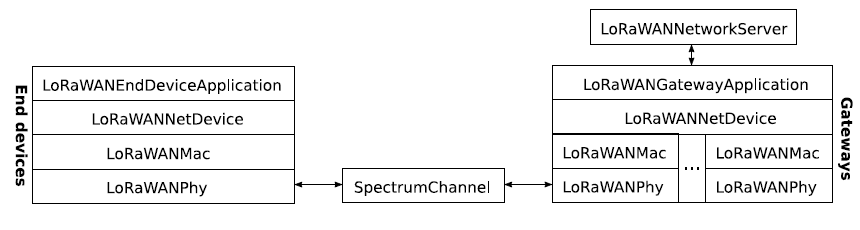
\includegraphics[scale=.5]{Immagini/ClasseA.png}

Fig. 10 Dispositivi di classe A, gateway e NS (server di rete).
\end{figure}
Quando un dispositivo terminale riceve una trasmissione downlink nella prima finestra, viene liberato dall'apertura della seconda finestra. Altrimenti, deve aprire la seconda finestra. Si noti che un dispositivo terminale ascolta sullo stesso canale e SF l'ultima trasmissione upstream nella prima finestra di ricezione (a meno che RX1DROffset non differisca da zero), mentre ascolta su un canale separato e SF12 nella seconda finestra. Inoltre, una classe A deve finire in attesa di trasmissioni upstream fino a dopo le finestre di ricezione. Infine, sia i messaggi upstream che downstream possono essere inviati come messaggi confermati e non confermati. I messaggi confermati vengono inviati utilizzando uno schema di ritrasmissione semplice a discrezione del dispositivo finale, senza violare le restrizioni del ciclo di lavoro. Le (ri)trasmissioni a downstream devono attendere una finestra di ricezione aperta e il loro timing è quindi controllato dal tempo di traffico a upstream di un dispositivo finale. Tuttavia, l'NS può impostare un bit di frame in sospeso in un messaggio downstream per segnalare a un dispositivo finale che potrebbe voler aprire una finestra di ricezione prima del normale \cite{art:rif.49}.

\subsubsection{Classe B – finali bidirezionali con finestre di ricezione programmate}
I dispositivi di Classe B LoRa forniscono le funzionalità dei classe A con l’aggiunta della possibilità di programmare intervalli di ricezione di informazioni in orari prestabiliti \cite{art:rif.27}. 
Per consentire al dispositivo finale di aprire la finestra di ricezione all'ora pianificata, riceve un segnale di sincronizzazione sincronizzata dal gateway. Ciò consente al server di sapere quando il dispositivo terminale è in ascolto \cite{art:rif.31}. 
La sincronizzazione temporale della rete avviene tramite l’invio di segnali regolari nel tempo dal gateway verso il nodo \cite{art:rif.27}.
\subsubsection{Classe C – finali bidirezionali con massimo numero di slot in ingresso}
I sensori Classe C LoRa permettono di avere il massimo livello di trasmissione server-nodo, ovvero, hanno finestre di ricezione quasi continuamente aperte, chiuse solo durante la trasmissione. La ricezione viene inibita solo nel momento in cui il nodo sta inviando informazioni verso la rete. Questa caratteristica rende i finali di Classe C particolarmente adatti alle reti LoRa caratterizzate da flussi di dati server-nodo superiori a quelli nodo-server \cite{art:rif.27}.

%% Un pacchetto LoRa è costituito da un preambolo, un'intestazione, un payload e un campo CRC. La specifica LoRaWAN identifica tre classi di dispositivi di Classe A, in cui i dispositivi finali utilizzano ALOHA puro per accedere al supporto per l'uplink. Questa classe è la più semplice e anche più comunemente usata. Supporta un collegamento verso valle solo in due finestre di ricezione (di default 1 s e 2 s) con un DR definito che segue una trasmissione di collegamento ascendente. I dispositivi di classe A hanno il consumo energetico più basso. I dispositivi di classe B possono inoltre utilizzare i segnali di beacon periodici emessi dai gateway per sincronizzarsi con la rete e programmare un'ulteriore finestra di ricezione. I dispositivi di classe C ascoltano sempre il canale quando non stanno trasmettendo. %

% Aggiungere una subsubsection con titolo, documento numero 18 %
\textbf{Nota Bene:} I nodi dei dispositivi finali contengono una singola coppia MAC / PHY, mentre i gateway sono costituiti da una coppia MAC / PHY per SF supportato. Ad esempio un gateway che supporta multi-SF (cioè, in grado di ricevere tutti gli LoRa SF contemporaneamente) su sei canali contiene 36 coppie MAC / PHY \cite{art:rif.49}.


\subsubsection{LoRaWAN PHY Layer}
La classe LoRaWANPhy è stata costruita sul concetto SpectrumPhy. La maggior parte dei modelli PHY impiegano un approccio basato sul segnale a un rapporto di rumore di interferenza (SINR) per modellare l'influenza della perdita di propagazione e interferenze intratecnologiche durante la ricezione di pacchetti. Ogni volta che il SINR cambia durante la ricezione dei pacchetti (ad esempio, una trasmissione interferente inizia o termina), viene avviato un nuovo blocco e il tasso di errore del blocco precedentemente ricevuto viene valutato in base al SINR costante e alla lunghezza di bit di questo blocco e al BER come fornito dal modello di errore. Si noti che LoRaWANPhy avvia solo la ricezione di pacchetti per le trasmissioni con un valore SINR al di sopra del valore di interruzione SNR. Le trasmissioni entranti che cadono sotto il valore di cut-off vengono immediatamente eliminate dal PHY. Oltre alla modellazione di ricezione, la classe LoRaWANPhy implementa anche una macchina a stati finiti per strutturare il suo flusso di esecuzione. L'FSM ha sei stati come mostrato in Figura. Le transizioni tra stati sono principalmente attivate dallo strato MAC (non mostrato nella figura). Negli stati RX\_ON e TX\_ON, il PHY è pronto a, rispettivamente, avviare una ricezione o trasmissione di pacchetti. Nello stato BUSY\_RX, il PHY è impegnato a ricevere una trasmissione (come per la suddetta ricezione a chunk, suddivisone del pacchetto in parti da 256 KB). Nello stato BUSY\_TX, il PHY sta inviando una trasmissione. Le ricezioni e le trasmissioni in corso possono essere annullate in qualsiasi momento, come indicato dalle transizioni di stato a TRX\_OFF. Si prevede che i PHY dei dispositivi di classe A rimangano per lo più in stato di inattività, mentre i PHY dei gateway dovrebbero essere nello stato RX\_ON per la maggior parte del tempo. Non ci sono differenze nelle classi PHY tra dispositivi e gateway di classe A. Pertanto, le differenze nella progettazione del ricetrasmettitore tra dispositivi terminali e gateway non vengono prese in considerazione in questo modello \cite{art:rif.49}.

\begin{figure}
\centering
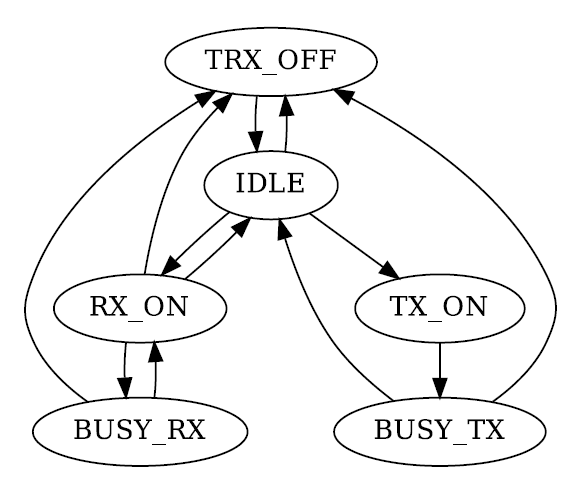
\includegraphics[scale=.5]{Immagini/MSFLoRaWAN.png}

Fig. 11 Macchina a stati finiti della classe LoRaWANPhy.
\end{figure}

\subsubsection{LoRaWAN MAC Layer} 
Il driver del livello PHY è la classe LoRaWANMac. La sua funzionalità include i pacchetti di accodamento per la consegna, l'apertura delle finestre di ricezione e la gestione delle ritrasmissioni sui dispositivi finali e la traccia dell'RDC di un nodo. Mentre esiste una classe LoRaWANMac per entrambi i dispositivi e gateway di classe A, la funzionalità di questa classe è diversa, ad esempio le ritrasmissioni per gateway sono gestite dall'NS. Allo stesso modo, il gateway MAC non ha il concetto di ricevere finestre poiché ascolta sempre il traffico upstream (quando non trasmette). Analogamente a LoRaWANPhy, la classe LoRaWANMac implementa anche un FSM come illustrato nella figura \cite{art:rif.49}. 

\begin{figure}
\centering
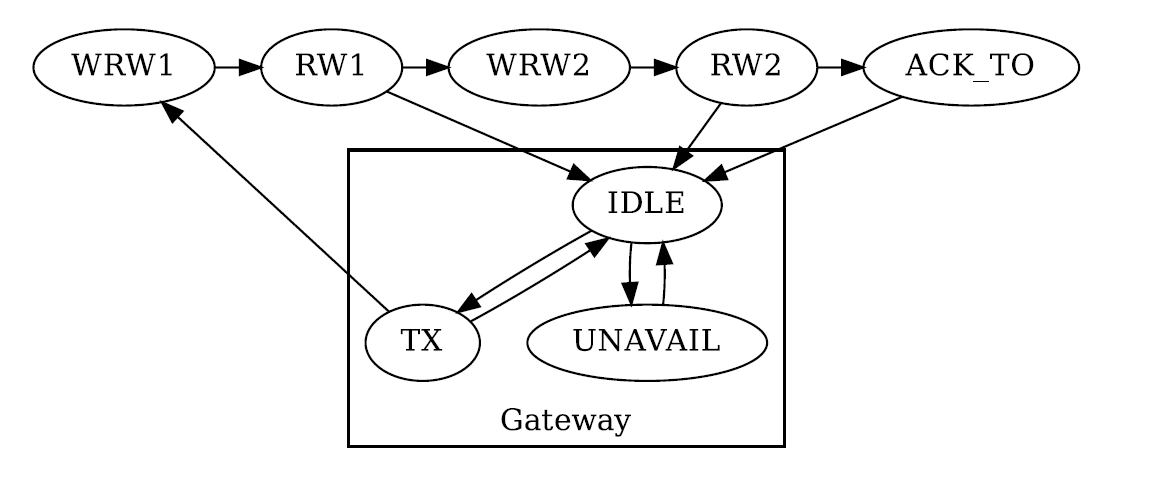
\includegraphics[scale=.3]{Immagini/MSFLoRaMAC.png}

Fig. 12 LoRaWANMac FSM è costituito da tre stati per gateway e sette stati per dispositivi finali di classe A.
\end{figure}

Mentre un oggetto MAC del dispositivo finale passa attraverso tutti gli stati, gli oggetti MAC del gateway sono limitati a tre stati. Lo stato UNAVAIL è un caso esclusivo dei gateway, in cui il MAC è bloccato dall'invio di un pacchetto. Questo stato viene attivato quando uno degli altri MAC sul gateway si trova nello stato TX, impedendo in tal modo le trasmissioni simultanee su diversi oggetti MAC sullo stesso gateway. La catena nella parte superiore della figura è correlata alle finestre di ricezione obbligatorie per i dispositivi di fine classe A nelle reti LoRaWAN. Dopo lo stato TX, un dispositivo terminale passa sempre allo stato WRW1. Il dispositivo finale spende 1 s (a partire dalla fine della trasmissione) in questo stato "wait for RW1", dopo di che apre RW1. Il dispositivo finale controlla se un preambolo PHY è stato ricevuto 12.25 simboli LoRa dopo l'inizio della finestra di ricezione. Se è stato rilevato un preambolo, il dispositivo continua a ricevere la trasmissione a downstream.
Se non è stato rilevato un preambolo, chiude la finestra di ricezione e passa allo stato WRW2. Se il dispositivo finale riceve correttamente una trasmissione downstream in RW1, passa allo stato IDLE. Altrimenti, chiude la finestra di ricezione e passa allo stato WRW2. Nello stato WRW2, il dispositivo terminale è in attesa di aprire la seconda finestra di ricezione (nello stato RW2) dopo 2 s dopo la fine della trasmissione. Lo stesso controllo del preambolo PHY da RW1 viene eseguito dopo l'apertura di RW2. Se viene ricevuta una trasmissione a downstream in RW2, il dispositivo terminale passerà allo stato IDLE. In caso contrario, potrebbe passare allo stato ACK\_TO (acknowledgement timeout) in cui trascorre un intervallo di tempo casuale prima di passare allo stato IDLE. Lo stato ACK\_TO viene visitato solo quando il dispositivo finale prevede un riconoscimento in una delle sue finestre di ricezione (ad esempio, dopo la trasmissione di un messaggio upstream confermato). Nel caso in cui non sia previsto un riscontro, il dispositivo passa direttamente allo stato IDLE da RW2. Le ritrasmissioni nel caso di dispositivi finali sono gestite interamente dalla classe LoRaWANMac. Finché il numero di trasmissioni rimanenti non è scaduto o non è stato ricevuto un frame downstream con il bit Ack impostato, un pacchetto di dati confermato rimarrà nella coda di trasmissione. Il numero di trasmissioni per i messaggi confermati può essere impostato tramite "DEFAULT\_NUMBER\_US\_TRANSMISSIONS" (in lorawan.h) ed è impostato su quattro per impostazione predefinita. Le (ri) trasmissioni successive vengono limitate in base alle limitazioni RDC della sottobanda attiva. A tal fine c'è un oggetto Singleton per nodo LoRaWAN, LoRaWANMacRDC, che tiene traccia del duty cycle di un nodo per le diverse sottobande. La classe LoRaWANMAC supporta anche l'invio di messaggi upstream non confermati più di una volta, come da linee guida nello standard LoRaWAN sul campo Numero di ripetizioni (NbRep). Questi messaggi rispediscono le limitazioni del ciclo di lavoro come qualsiasi altra normale trasmissione. Infine, la classe LoRaWANMac aggiunge 1B LoRaWANMacHeader (che codifica il tipo di messaggio) e un 4B dummy MIC al payload MAC prima di passare il pacchetto al PHY \cite{art:rif.49}.

\subsubsection{Dati non confermati e confermati in upstream}
La rete LoRaWAN a singolo Gateway considera nel PDR l'impatto dell'invio di dati in upstream come messaggi MAC confermati. Ci si aspetterebbe che lo schema di ritrasmissione LoRaWAN aumenti il PDR, in quanto i messaggi non riconosciuti vengono ritrasmessi dal dispositivo finale. Nel caso di messaggi confermati, un dispositivo terminale tenta quattro trasmissioni prima di rilasciare il messaggio. In ogni momento, i dispositivi terminali rispettano le restrizioni del ciclo di lavoro. Il PDR diminuisce quando i dati vengono inviati con maggiore frequenza e con l'aumento del numero di dispositivi finali. In caso di messaggi MAC non confermati, la causa principale dei pacchetti non consegnati è dovuta a collisioni in cui il gateway è impegnato a ricevere una trasmissione e quindi qualsiasi altra trasmissione con la stessa velocità dati viene eliminata durante la ricezione in corso. Per il periodo di dati di 600 s, la quota di pacchetti non consegnati e scartati dovuta a collisioni è vicina al 90\%. Un altro 9\% dei pacchetti non consegnati viene scartato a causa di interferenze durante la ricezione. Il resto dei pacchetti non consegnati viene eliminato a causa di un valore SINR che scende al di sotto del punto di interruzione SNR. Mentre inviando messaggi non confermati quattro volte aumenta il PDR per gli scenari a basso traffico, il PDR è inferiore negli scenari in cui l'interferenza diventa il fattore limitante. Si noti che la percentuale di velocità di trasmissione più lenta nei pacchetti non consegnati è superiore a quella delle velocità di trasmissione più veloci. Ciò è in parte dovuto alla maggiore quota di dispositivi finali con velocità di trasmissione dati più basse nelle reti e parzialmente a causa dei tempi di trasmissione più elevati a velocità di trasmissione inferiori. Un po' controintuitivamente, il PDR dei messaggi confermati non è sempre superiore a quello dei messaggi non confermati. Il PDR dei messaggi CON è solo superiore a quello di UNC (unconfirmed) nei casi in cui il carico del traffico è molto basso. Nelle simulazioni questo è solo il caso per 100, 500 e 1000 dispositivi terminali per un periodo di dati di 60 000 s e per 100 dispositivi terminali per un periodo di dati di 6000 s. In tutti gli altri casi il PDR dei messaggi confermati è inferiore. Ricorda che un messaggio confermato viene considerato consegnato solo se il dispositivo finale riceve un riconoscimento per quel messaggio. Il numero di finestre di ricezione perse (per l'invio di una conferma) aumenta con l'aumentare del carico di traffico. Le finestre di ricezione vengono perse perché il gateway non è in grado di trasmettere all'inizio di una finestra di ricezione a causa delle restrizioni del ciclo di lavoro che si applicano nella sottobanda di una finestra di ricezione. Mentre CON (confirmed) e 4UNC (4 unconfirmed) hanno carichi di traffico simili per reti saturate, il PDR dei messaggi CON è inferiore a quello di 4UNC. Questa differenza è spiegata dalle mancate conferme downstream per i messaggi CON. Infine, quando un gateway invia una conferma in RW1 o RW2, tutte le ricezioni in corso sul gateway vengono interrotte; che diminuisce ulteriormente il PDR. 
Le reti multigateway LoRaWAN grazie all'utilizzo di un maggior numero di gateway ottiene un miglioramento sul PDR. Si noti che per l'applicazione della strategia di allocazione SF PER 0,01, il PER al gateway più vicino viene calcolato per ogni dispositivo finale. Si prevede che l'aumento della densità del gateway abbia più di un effetto. In primo luogo, dovrebbe consentire velocità di trasmissione dati più elevate per i dispositivi finali a causa di un aumento del budget di collegamento (poiché i gateway medi appariranno più vicini). In secondo luogo, poiché le trasmissioni downstream in RW1 vengono inviate con la stessa velocità dati delle trasmissioni upstream, i riconoscimenti RW1 dovrebbero anche beneficiare delle maggiori velocità dati dei dispositivi finali. Infine, poiché le restrizioni del ciclo di lavoro si applicano per gateway, la rete LoRaWAN dovrebbe essere in grado di riconoscere più messaggi man mano che la densità del gateway aumenta. Si noti come per i messaggi non confermati, il PDR aumenta notevolmente all'aumentare del numero di gateway. Per i messaggi confermati, l'aumento del PDR è notevole ma non è così acuto come per i messaggi non confermati. Il numero di conferme inviate aumenta con l'aumentare del numero di gateway. La relazione apparentemente contraddittoria tra il numero di RW persi e il numero di gateway è spiegata come segue. Nelle reti LoRaWAN saturate (ad esempio, scenari con PDR bassi per messaggi non confermati), il numero di messaggi inviati ricevuti con successo aumenta con la densità del gateway. In caso di messaggi confermati, il numero più alto di messaggi upstream ricevuti indica che NS è in grado di identificare un numero maggiore di finestre di ricezione dei dispositivi finali (poiché gli RW vengono sempre aperti dopo una trasmissione di un dispositivo finale). Quando i gateway non sono in grado di inviare queste finestre di ricezione (a causa delle restrizioni del ciclo di lavoro), il numero di RW persi aumenta. In scenari meno saturi, il numero di RW persi diminuisce all'aumentare della densità del gateway non porta a identificare più finestre di ricezione. Invece, il numero di RW persi diminuisce e vengono inviati più riconoscimenti, a vantaggio del PDR.
I risultati mostrano che i messaggi confermati hanno un impatto grave sui rapporti di consegna dei pacchetti dei messaggi a upstream. Mentre aumentare il numero di gateway aiuta ad alleviare questo problema in qualche modo, i risultati del periodo di dati di 600 s mostrano che il PDR rimane basso anche in una rete di quattro gateway. L'impatto dei messaggi di dati in downstream sui messaggi in upstream è risultato trascurabile a causa della scarsità del carico di traffico di dati in downstream (sporadiche notifiche). Inoltre, è stata trovata una piccola differenza tra l'invio di dati downstream come messaggi non confermati rispetto ai messaggi confermati in termini di downstream PDR. L'approccio di modellizzazione di tutte le interferenze come rumore ha i suoi svantaggi. Nello specifico, la letteratura ha dimostrato che mentre l'interferenza tra diversi SF può essere modellata accuratamente come rumore, l'interferenza co-SF può essere modellata in modo più accurato tramite un approccio stocastico. Quando i messaggi di dati downstream non vengono recapitati a causa delle limitazioni RDC (anziché della bassa qualità del collegamento), una velocità di trasmissione dati RW2 più rapida potrebbe aumentare la capacità del LoRaWAN \cite{art:rif.49}. 

\subsection{Protocollo IP / Lv 3} 
Rispetto agli altri standard, una rete LoRa è IP-based compatibile con IPv6, una caratteristica essenziale per ogni sviluppo di nuovi progetti IoT. Una rete LoRa comprende dei gateway per la connessione al server centrale di rete. Gli end-point comunicano con una topologia di rete a stella mediante un collegamento wireless single-hop ai gateway con la possibilità di collegarsi a più gateway, per garantire la ridondanza del collegamento. Per coprire una grande area è sufficiente un'infrastruttura leggera \cite{art:rif.20}. 
Scendendo nel dettaglio l'architettura di una rete LoRa prevede una tipologia a stella di stelle in cui il Gateway è un bridge trasparente per i messaggi tra Devices e il Network Server. I Gateway sono connessi al Network server tramite una connessione basata sollo standard IP, mentre i Device utilizzando una comunicazione wireless single-hop verso uno o più Gateway. La comunicazione verso i Device è in generale bidirezionale, ma può anche supportare il muticast per gestire l'aggiornamento o la distribuzione massiva di messaggi per ridurre i tempi di comunicazione \cite{art:rif.25}.
Il cuore di ogni concentratore LoRa è un demodulatore LoRa multi-canale in grado di decodificare tutte le varianti di modulazione LoRa su più frequenze in parallelo. Un demodulatore LoRa standard per dispositivo terminale (LoRa modem come SX1276 o SX1272) può decodificare un solo tipo di modulazione su una frequenza. Attualmente, il demodulatore LoRa ampiamente utilizzato è SX1301 di Semtech. Questo chip è integrato in tutti i gateway LoRa nel nostro attuale portafoglio. A causa del crescente numero di produttori di gateway, sta diventando difficile individuare le differenze tra i gateway. Per un operatore di rete su larga scala, i principali fattori di distinzione dovrebbero essere le prestazioni radio (sensibilità, potenza di invio), la connessione del chip SX1301 all'MCU gateway e il supporto e la distribuzione del segnale PPS. SX1301 collegato su un bridge da USB a SPI ha una latenza più lunga sull'MCU rispetto a un SX1301 direttamente collegato al bus SPI dell'MCU. Attualmente, l'unico SPI collegato SX1301 si trova nella stazione IoT Kerlink, tutti gli altri gateway utilizzano ponti USB-to-SPI FTDI (o simili). La disponibilità del segnale PPS consente una sincronizzazione temporale precisa sull'intera popolazione di gateway in una rete. È un attivatore chiave per i beacon a livello di rete, che può essere utilizzato per la sincronizzazione dell'ora da parte dei dispositivi finali. La distribuzione PPS è attualmente supportata solo dalla stazione IoT Kerlink, dalla scheda di riferimento SX1301 e dall'IMST iC880A \cite{art:rif.30}. 

\subsection{Applicazioni LoRa / Lv 7}
LoRa Technology sta connettendo il nostro pianeta intelligente. Esistono una moltitudine di applicazioni verticali IoT e implementate in tutto il mondo \cite{art:rif.24}.
I gateway inoltrano i frame ricevuti a un server di rete cloud ospitato da AWS (CNS). Il sistema CNS procede a un primo filtraggio dei frame ricevuti tramite over-the-air. In questa fase vengono elaborati solo i frame con un CRC valido. Dal CNS basato su AWS, trasfersce i dati attraverso MQTT a una pipeline di elaborazione. Quest'ultimo consiste in un OpenTSDB che consuma valori di sensori e li memorizza in un database. È implementata un'interfaccia utente e una serie di API per estrarre e visualizzare i dati da OpenTSDB. Quando si memorizzano i dati su OpenTSDB, si applica un secondo livello di filtraggio ottenuto applicando le condizioni al contorno alle letture e ai valori dei sensori. La necessità di applicare queste condizioni al contorno deriva dal fatto che si possono verificare errori nella lettura del sensore, che provenivano da guasti intermittenti sul sensore stesso o da byte over-air che cambiano, ma che arrivavano con un buon CRC che genera dati di sensore errati \cite{art:rif.43}.
Un aspetto di notevole importanza per le applicazioni IoT è la criptazione di sicurezza incorporata nelle reti LoRa, che consente ai livelli applicazione e dispositivo di offrire una struttura di protezione dei dati personali o delle funzioni critiche dagli attacchi fisici o informatici \cite{art:rif.20}. 
La questione della sicurezza della rete sta diventando sempre più importante, pertanto le reti LoRa richiedono elevati livelli di sicurezza. Il raggiungimento dei necessari standard di sicurezza per le reti LoRa viene ottenuto impiegando diversi livelli di crittografia:
\begin{enumerate}
\item chiave univoca di rete (EUI64) che garantisce la sicurezza a livello di rete;
\item chiave unica di applicazione (EUI64) per garantire la sicurezza end-to-end a livello di applicazione;
\item chiave specifica del nodo finale (EUI128).
L’impiego di questi livelli di crittografia assicura che la rete LoRa rimanga sicura lungo tutto il percorso, dal nodo fino all’applicazione \cite{art:rif.27}.
\end{enumerate}
Esistono due gruppi di domini crittografici in LoRa: il dominio di rete e il dominio dell'applicazione. Il dominio di rete è responsabile dell'autenticazione dei dati del nodo finale. La paternità di tali dati è verificata tramite una chiave segreta AES128 condivisa tra il dispositivo e il server di rete. Il dominio dell'applicazione è responsabile della garanzia della riservatezza dei dati del dispositivo. Esiste una chiave segreta AES128 condivisa tra l'applicazione utente e il nodo finale. LoRa è la soluzione più sicura disponibile sul mercato con crittografia 128AES su più livelli per tutti i dati dal sensore al server delle applicazioni e viceversa \cite{art:rif.30}.
Il software Long Range Signaling and Control (LRSC) di IBM e al servizio sul cloud IBM Internet of Things Foundation, la LoRaWAN consente una facile implementazione su vasta scala di M2M/IoT. L'LRSC è il middleware o il collante che consente agli utenti di collegare, gestire e scalare milioni di dispositivi. IBM ha inoltre reso il protocollo LoRaWAN open source (Eclipse Public License) per lo sviluppo del nodo finale conosciuto come "LoRaWAN in C" \cite{art:rif.26}.


%% La specifica LoRaWAN ™ definisce un framework di sicurezza a doppio strato (chiavi di sessione di applicazioni e di rete) che adotta la crittografia AES nota da IEEE 802.15.4. %

\subsubsection{LoRaWAN Applicazione del End Device}
L'applicazione LoRaWANEndDeviceApplication viene descritta per rappresentare i dispositivi finali di classe A LoRaWAN. L'applicazione espone gli attributi per parametri come la velocità dati del dispositivo finale e la lunghezza del pacchetto e il tipo di messaggio delle trasmissioni upstream. Supporta anche variabili casuali configurabili per la selezione del canale upstream e per i tempi di generazione del pacchetto. L'applicazione è responsabile della generazione del payload MAC, in quanto tale aggiunge l'intestazione del frame LoRaWAN al payload dell'applicazione. Questa intestazione del frame codifica l'indirizzo del dispositivo finale, il contatore dei pacchetti e la porta del frame dell'applicazione. I metadati relativi alla trasmissione dei pacchetti, come il canale desiderato, la velocità dei dati e la velocità del codice, vengono trasmessi al PHY tramite un tag del pacchetto LoRaWANPhyParamsTag \cite{art:rif.49}.

\subsubsection{Applicazione LoRaWAN Gateway}
LoRaWANGatewayApplication è una semplice applicazione, ovvero installata sui nodi gateway. Oltre a passare pacchetti e accettare pacchetti dal NS, supporta anche l'interrogazione dello stato RDC di un gateway dal NS. I pacchetti che devono essere inviati a downstream sono etichettati con il tag del pacchetto LoRaWANPhyParamsTag dal NS. LoRaWANNetDevice sul gateway selezionerà la coppia MAC / PHY corrispondente agli attributi PHY che sono elencati nel tag del pacchetto (cioè, SF e canale) \cite{art:rif.49}.

\subsubsection{LoRaWAN Network Server}
Questo oggetto singleton accetta i pacchetti upstream dai gateway e invia il traffico downstream ai dispositivi finali tramite gateway. Espone i seguenti attributi per configurare la generazione del traffico downstream:
\begin{enumerate}
\item dimensione del pacchetto;
\item messaggi confermati o non confermati;
\item variabile casuale per la generazione di pacchetti.
\end{enumerate}
La classe tiene traccia delle informazioni come l'indirizzo del dispositivo, i contatori dei pacchetti, l'ultima velocità dati, l'ultimo gateway $(i)$ noto e l'ultimo tempo visto per ogni dispositivo finale. Basato sui contatori di pacchetti, è in grado di rilevare pacchetti di dati duplicati da più gateway. L'NS genera dati e riconoscimenti a downstream. A tal fine, contiene una coda di pacchetti di dispositivi per end per la memorizzazione del traffico downstream. Per ogni dispositivo finale, memorizza i timer RW1 e RW2 utilizzati per la pianificazione del traffico downstream. Quando un timer scade, l'NS passa attraverso l'elenco degli ultimi gateway noti e cerca un gateway che possa inviare immediatamente il pacchetto downstream in coda. Questi timer sono programmati ogni volta che una trasmissione upstream viene elaborata dal NS. Infine, l'NS si occupa delle ritrasmissioni per i pacchetti di dati a downstream confermati \cite{art:rif.49}.

\subsubsection{Adaptive Data Rate}
La capacità di controllare i parametri di trasmissione, inclusi lo schema di modulazione e la potenza di uscita, consente di ridurre i costi di implementazione, migliorare l'affidabilità della rete, in termini di prestazioni degli errori in condizioni subottimali e potrebbe contribuire alla riduzione della complessità della manutenzione rispetto al ridimensionamento il network. L'algoritmo ADR (Adaptive Data Rate), ampiamente accettato utilizzato nelle attuali infrastrutture di rete basate su LoRaWAN, è un meccanismo per ottimizzare la velocità di trasmissione dati, tempo di trasmissione e consumo energetico nella rete. 
I parametri di trasmissione wireless negli spettri non licenziati sono regolati a livello regionale con aggiunte occasionali da parte dei regolatori del paese. Normalmente i regolamenti includono, ma non sono limitati a, la definizione di potenza massima irradiata efficace (ERP, effective radiated power) e duty-cycle, e metodi di accesso medio. Sebbene più trasmissioni LoRa emesse simultaneamente possano essere elaborate da un singolo gateway sfruttando l'ortogonalità dei fattori di diffusione oltre all'uso di più sotto-bande di trasmissione, la natura dell'accesso ALOHA al mezzo porta inevitabilmente alla presenza di collisioni di trasmissione. La dipendenza esponenziale del TOA su SF introduce un limite superiore esponenziale alle prestazioni della rete. Il throughput della rete è legato in alto o dalla velocità di collisione (DR inferiore, TOA più breve) o dalla limitazione del ciclo di lavoro (DR più alto, TOA più lungo). I sistemi che contengono i nodi finali i cui parametri di trasmissione sono costanti rispetto al tempo sono particolarmente interessati. L'implementazione di uno schema di trasmissione dinamica, ad esempio ADR in LoRaWAN, e di addensare l'infrastruttura aggiungendo ulteriori gateway. Poiché, come visto dagli operatori di rete, l'implementazione di un ADR è un modo efficiente CAPEX per ottimizzare la capacità delle reti, i fornitori che offrono NM sul mercato mantengono i loro algoritmi come parte della proprietà intellettuale. Contrariamente a questa tendenza, la disponibilità generale da parte dei clienti dei prodotti LoRaWAN ha catalizzato la creazione di numerosi progetti di implementazione NM open source che includono il TTN (The Things Network) e un LoRa Server più giovane, i cui algoritmi ADR sono disponibili pubblicamente \cite{art:rif.48}.

Solo i nodi statici dovrebbero utilizzare ADR. L'ADR può anche essere utilizzato da un nodo mobile che è in grado di rilevare quando è "posizionato" su un punto fisso. I nodi decidono se utilizzare o meno l'ADR, non l'applicazione o la rete. Dal momento in cui un nodo indica che desidera utilizzare ADR, la rete raccoglierà le metriche delle 20 trasmissioni più recenti dal nodo. Questa cronologia contiene il contatore di frame, il rapporto segnale-rumore (SNR, signal-to-noise ratio) e il numero di gateway che hanno ricevuto ciascuna trasmissione. In questo modo la rete può calcolare quanto "margine" c'è per aumentare la velocità dei dati o ridurre la potenza di trasmissione. Ad esempio, quando la rete riceve un messaggio con velocità dati = $SF12BW125$ e $SNR = 5.0$, tale messaggio ha un margine di 25 dB. Questo è uno spreco di prezioso tempo di trasmissione ed energia. Se aumentassimo la velocità di trasmissione dati a $SF7BW125$ avremmo ancora un margine di 12,5 dB, ma ciò sarebbe molte volte più efficiente in termini di tempo ed energia. Potremmo persino abbassare la potenza di trasmissione per risparmiare ancora più energia e causare meno interferenze. L'algoritmo utilizzato in The Things Network si basa sull'algoritmo consigliato da Semtech per l'adattamento della frequenza. Lo schema in figura 13 delinea il flusso ADR implementato nel NetworkServer di The Things Network \cite{art:rif.32}.

\begin{figure}
\centering
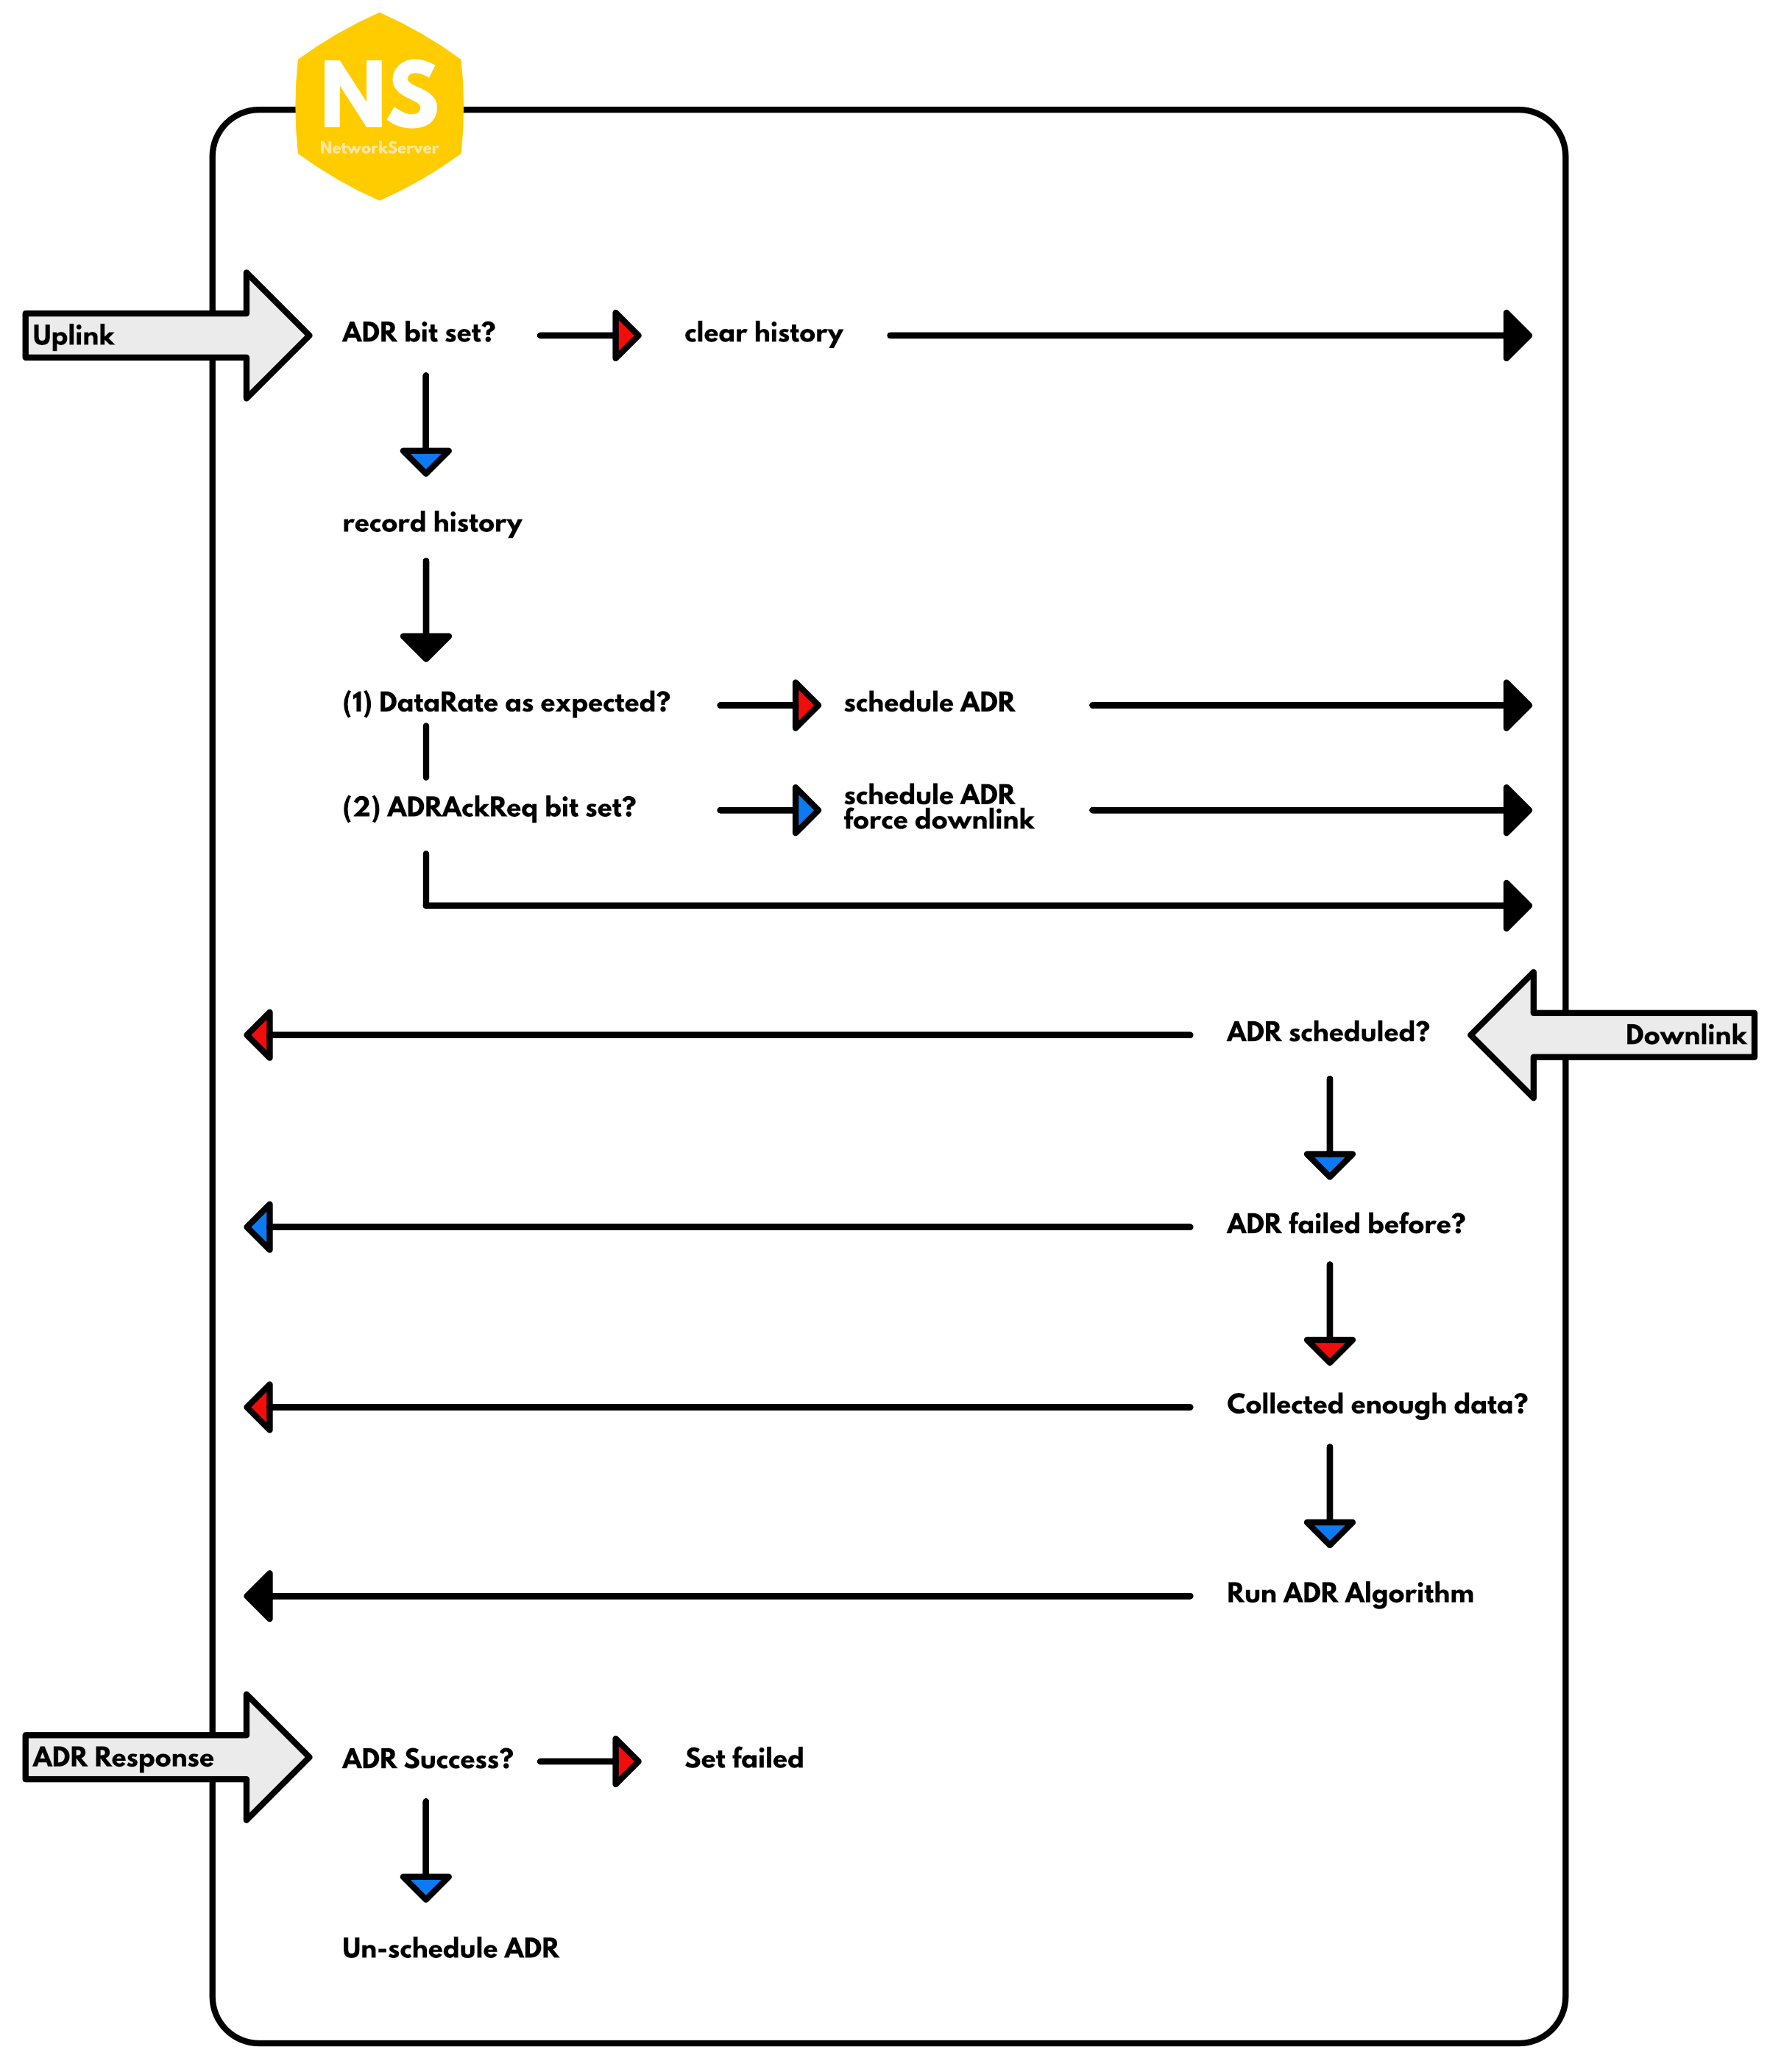
\includegraphics[scale=.5]{Immagini/adr.png}

Fig. 13 Figura schema del flusso ADR.
\end{figure}

La parte della specifica LoRaWAN dedicata ai comandi relativi ad ADR delinea la seguente procedura che il dispositivo finale dovrebbe seguire per ottenere una velocità di trasmissione dati ottimale. Inizialmente, il dispositivo terminale deve richiedere l'adattamento della velocità di trasmissione dati da NM (Network Manager) impostando il bit ADR in un'intestazione di messaggio uplink. Successivamente il dispositivo terminale regola il suo DR, il livello di potenza di trasmissione, la frequenza di ripetizione dei frame non confermati e l'insieme dei canali di uplink consentiti in base ai comandi MAC LinkADRReq ricevuti. Il dispositivo finale conferma ogni parte della configurazione richiesta su NM in un comando MAC LinkADRAns. Poiché l'impostazione eccessivamente ottimistica del DR può rendere irraggiungibile il dispositivo end-end, la specifica LoRaWAN definisce una seguente procedura di salvaguardia: se un dispositivo terminale non riceve alcun downlink all'interno di ADR\_ACK\_LIMIT uplink e il DR corrente è maggiore del DR minimo, tutti gli uplink successivi vengono inviati con il set di bit di riconoscimento ADR (ADRACKReq) impostato. Se il dispositivo finale non riceve alcun downlink entro i successivi uplink ADR\_ACK\_DELAY, il dispositivo terminale potrebbe provare a riguadagnare la connettività passando al successivo DR inferiore fornendo un intervallo esteso. Successivamente, ogni volta che viene raggiunto ADR\_ACK\_DELAY, il dispositivo terminale riduce il DR di un gradino. L'end device utilizza un contatore interno (ADR\_ACK\_CNT) che viene ripristinato alla ricezione di ogni messaggio di downlink \cite{art:rif.48}.

\subsection{Misura delle prestazioni LPWAN}
I tre principali parametri che incidono sulle prestazioni di LPWAN (in termini di ritardo end-to-end e tasso di perdita di pacchetti) sono: 
\begin{enumerate}
\item la performance di LPWAN è influenzata anche da un piccolo grado di mobilità (cioè, la mobilità umana);
\item L'effetto della mobilità è maggiore in un ambiente interno;
\item La maggiore distanza dal gateway aumenta ulteriormente il impatto della mobilità.
\end{enumerate}
Questi risultati suggeriscono che c'è bisogno di un nuovo mobilityaware. I protocolli LPWAN devono essere sviluppati e migliorati per reti con host mobili \cite{art:rif.25}.

\subsection{Compressione dei dati}
L'esigenza di gestire enormi quantità di dati porta con se due argomenti da trattare, compressione e sicurezza del trasferimento dei dati. La codifica Swapped Huffman tree (SHT) applicata ad una rete a bassa potenza (LPWAN) comprime e codifica i dati allo stesso tempo.
Il problema con LPWAN è che funziona su una larghezza di banda ridotta che crea un problema di comunicazione dati limitata. A causa di questa limitazione, la comunicazione può avvenire sotto forma di pacchetti di testo ma non di immagini o video. Tuttavia, nell'IoT, è necessario effettuare grandi quantità di trasferimento dei dati che richiede la necessità della compressione dei dati per trasmettere i dati necessari. In secondo luogo, i dati compressi richiedono una trasmissione sicura, a causa della quale è richiesta anche la crittografia dei dati. Per affrontare questi problemi, si può implementare la codifica Swapped Huffman tree (SHT) su una rete magliata.
È estremamente importante per qualsiasi LPWAN incorporare la sicurezza per garantire la sicurezza dei dati dell'applicazione dell'utente in IoT, nella tecnologia LoRa la comunicazione viene eseguita utilizzando lo standard avanzato di crittografia (AES).  Insieme all'utilizzo della crittografia dei dati, un altro fattore chiave nell'IoT, come accennato in precedenza, è la compressione dei dati.
Ad oggi i ricercatori hanno proposto un numero di metodi di compressione dei dati per gestire i problemi dei big data per IoT, tra cui metodi per la compressione dell'header di DTLS (datagram transport transport security, protocollo) per il suo utilizzo nella sicurezza end-to-end di IoT. Poiché nell'IoT ci sono diversi nodi di sensori per eseguire la compressione dei dati di questi nodi, è stato proposto uno schema di compressione dei dati del sensore adattativo (ASDC, adaptive sensor data compression) \cite{art:rif.45}. 

\subsubsection{Codifica Swapped Huffman Tree}
La codifica di Huffman è un particolare tipo di codice di prefisso ottimale comunemente usato per la compressione senza perdita di dati. Dato che la codifica di Huffman non è crittografata, l'abilità di crittografia viene introdotta dagli stessi ricercatori, cioè la mutated Huffman table (MHT) e la chaotic Huffman table(CHT). MHT ha perso il suo significato di crittografia perché i ricercatori hanno eseguito un'analisi che mostra che è vulnerabile agli attacchi. Quindi, è apparso SHT successivo che è più affidabile della tecnica MHT. In SHT, la crittografia e la compressione vengono eseguite insieme; la parte di compressione è basata sulla codifica di Huffman. Per la parte di crittografia, utilizza la tecnica chiamata Mutation su Huffman Coding. La mutazione è l'interruttore tra le etichette del ramo del nodo dell'albero, cioè da '0' a '1' e '1' a '0', come in figura 1. SHT è più affidabile della tecnica MHT perché non solo usa mutazione per la crittografia ma anche il meccanismo di scambio della chiave di crittografia. È un meccanismo in cui la mutazione viene eseguita più volte dividendo il flusso chiave totale in ulteriori segmenti chiave in base alla dimensione dei bit indicati, come in figura 2. , dove $T^{(k)}$ rappresenta il numero di mutazione dell'albero. Il numero di bit in ogni segmento è deciso in base al numero di nodi nell'albero di Huffman. Ogni segmento viene applicato all'albero in modo che se si verifica "1", quel nodo viene mutato e se "0", il nodo viene lasciato così com'è. La lunghezza della chiave di crittografia segreta non ha limitazioni che la rendono resistente agli attacchi di forza bruta. Inoltre, non influisce sul rapporto di compressione dopo la crittografia. Supponiamo di avere un testo piano come \{$S_1$ $S_2$ $S_4$ $S_5$ $S_2$ $S_3$ $S_6$ ......\}. Se consideriamo che la chiave di crittografia segreta è: \{001100101011\} quindi da figura 3 il codice del testo piano è: \{1011001000110111001 ......\}. Se usiamo l'albero base $T^{(0)}$ in figura 3 per decodificare il testo cifrato, otteniamo \{$S_4$ $S_5$ $S_2$ $S_1$ $S_5$ $S_6$ $S_1$ ......\}, che è completamente diverso dal testo del piano originale. Dopo aver compreso la codifica SHT e la parte relativa alla mutazione, la prossima sezione fornisce l'implementazione del software \cite{art:rif.45}.
\begin{figure}
\centering
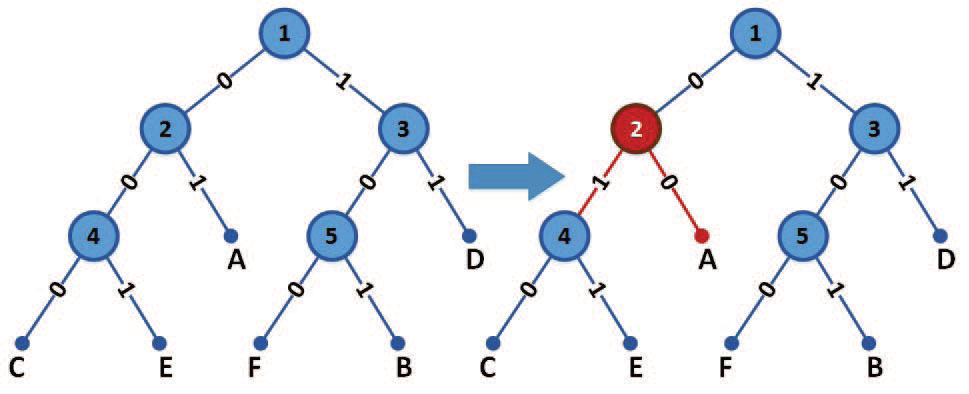
\includegraphics[scale=.4]{Immagini/SHT1.png}
Fig. 14 1 Huffman Tree
\end{figure}

\begin{figure}
\centering
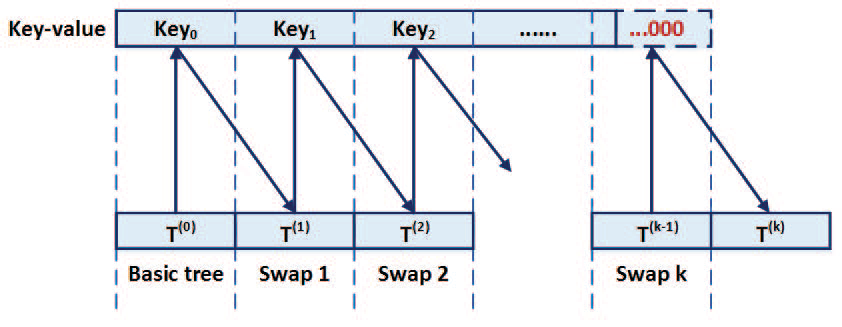
\includegraphics[scale=.5]{Immagini/SHT2.png}
Fig. 15 2 Tree Swapping
\end{figure}

\begin{figure}
\centering
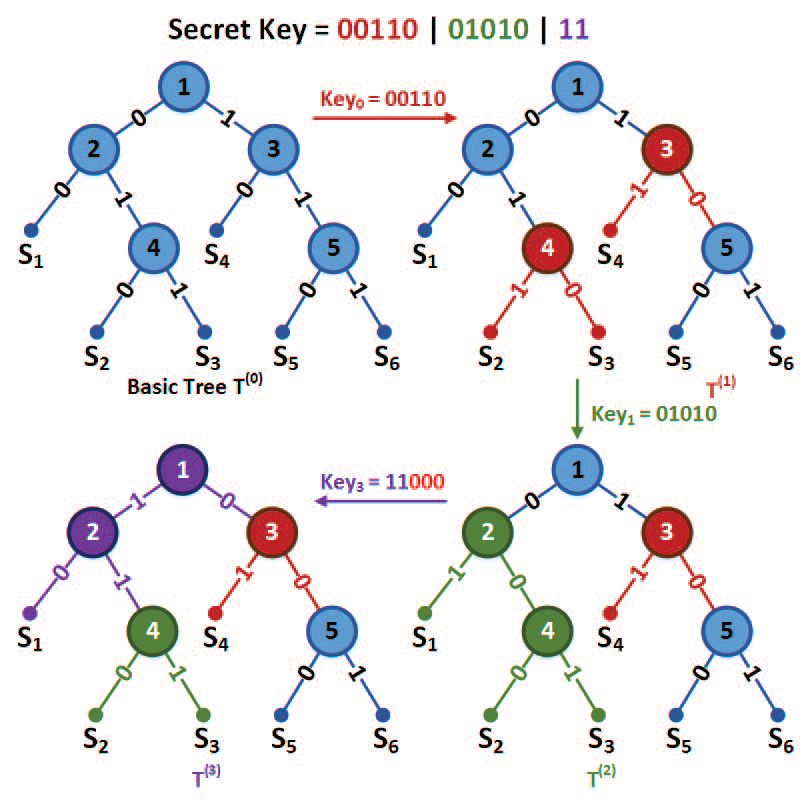
\includegraphics[scale=.5]{Immagini/SHT3.png}
Fig. 16 3 Esempio SHT
\end{figure}

\subsubsection{Implementazione della mutazione}
La codifica di Huffman è già implementata in vari linguaggi di programmazione. Tra questi, c'è il codice C come alternativa. Poiché non è facile mutare i nodi dell'albero nell'implementazione del codice, quindi è stato proposto un modo alternativo usando C.

\begin{lstlisting}
Input: Original-Code, Encryption-Key
Output: Mutated-Code MC

char* function mutation{
	check = maxlength (OCs);
	while (maxlength (maked) = = check){
		making(' ', '0', '1', '00', '01', '10', '11', ...)
		}
	for (i = 0; i < count (maked); i++){
		if ((OC != maked) or (OC_and maked_is_completely_same)){
			that_maked_delete;
		}
	}
	divided Encryption-Key according to count (maked);
	for (j = 0; j < count (maked); j++){
		if (OC_left = = maked){
			OC_left's_next = toggle;
		}
	}
	return OC;
	goto NextCode;
}
\end{lstlisting}

Lo pseudocodice implementa la mutazione nella codifica SHT. L'implementazione C alternativa proposta del processo di crittografia viene fornita in quattro fasi come segue:
\begin{enumerate}
\item Definire la chiave cifrata segreta e dividerla in segmenti M.
\item Definire una lista di controllo usando i simboli "S" dell'albero $T^{(n)}$ dove n = \{0, 1, ..., M-1\}.
\item Utilizzare l'elenco di controllo nel passaggio 2 insieme al segmento di codice cifrato corrispondente nel passaggio 1 per eseguire la crittografia.
\item Passare al punto 2 e ripetere il processo fino a quando non viene raggiunto l'ultimo segmento della chiave di cifratura.
\end{enumerate}

Per la generazione di $T^(1)$ crittografato dall'albero base $T^{(0)}$ (Figura 3):
\begin{enumerate}
\item Definizione della chiave di cifratura segreta e segmentazione:
Dalla Fig. 3, abbiamo \{001100101011\}. Quindi il numero di segmenti è M = 3, cioè, \{00110 | 01010 | 11000\}.
\item Definizione dell'elenco di controllo: il processo è il seguente:

\begin{enumerate}
\item Definire la lunghezza massima di ciascun simbolo nella checklist $l = k -1 bits$, dove k è il numero massimo di bit nei simboli $T^{(n)}$, ad esempio, in Fig. 3, per $T{^(0)}$ nessuno dei simboli S ha più di tre bit, quindi $l = 3 -1 = 2 bits$. 
\item Secondo $l$ al punto 1, definire l'elenco di controllo a partire da \{'', 0, 1, 00, 01, 10, 11, 000, 001, ......\}, ad esempio, in figura 3, $l = 2 bits$ quindi la lista è \{'', 0, 1, 00, 01, 10, 11\}.
\item Una volta creata la lista di controllo, affinarla, confrontarla con l'elenco dei simboli dell'albero corrispondente e rimuovere i codici uguali o non presenti nell'elenco dei simboli, ad es. In Fig. 3, la lista dei simboli per $T^{(0)}$ è \{$S_1$, $S_2$, $S_3$, $S_4$, $S_5$, $S_6$\} = \{00, 010, 011, 10, 110, 111\}, vediamo che 00 e 10 nella lista generata nel passaggio (b) esistono anche in la lista dei simboli, quindi la checklist finale sarà \{'', 0, 1, 01, 11\}.
\end{enumerate}

\item Applicazione della lista di controllo: per $T^{(0)}$ in figura 3, il primo segmento, 00110, della chiave di cifratura nella fase 1 verrà applicato insieme alla lista di controllo perfezionata generata fase 2, cioè, \{'', 0, 1, 01, 11\}. Per gli "0" nel segmento chiave cifrario ignorare la mutazione e per 1s eseguire la mutazione. Ora per la mutazione dell'elenco di controllo, prendi uno per uno ciascun simbolo della lista di controllo e confrontalo con i più significativi (MSB) dell'elenco simboli. Se i MSB sono uguali, commuta il bit successivo immediato sui MSB, cioè da 0 a 1 o da 1 a 0. Eseguilo su tutti i simboli nella lista dei simboli dell'albero $T_{(0)}$. Dopo la mutazione che utilizza il segmento chiave cifrario e l'elenco di controllo, i simboli crittografati generano $T_{(1)}$. Esiste solo un'eccezione che se il primo bit del segmento della chiave di cifratura è 1, verrà selezionato \{''\} dalla checklist, in questo caso bisogna commutare tutti gli MSB di ciascun simbolo nell'elenco di simboli.

\item Dopo la generazione di $T^{(1)}$ passare al punto (c) del passaggio 2 e usare $T^{(1)}$ anziché $T^{(0)}$ come albero base per la generazione di $T^{(2)}$. Ora questa volta verrà utilizzato il prossimo segmento della chiave di cifratura, ad esempio dalla figura 3, per la generazione di $T^{(2)}$ da $T^{(1)}$ verrà usato il segmento 01010 e così via. Ripeti fino al raggiungimento del segmento finale della chiave di cifratura \cite{art:rif.45}.
\end{enumerate}

\subsubsection{Prestazioni della codifica di Huffman}
La valutazione delle prestazioni della compressione e della crittografia utilizzando la codifica SHT per le reti a bassa velocità viene eseguita presupponendo che il trasmettitore e il ricevitore siano a conoscenza della tabella di codici di Huffman che è stata determinata in anticipo. La valutazione di entrambe le parti, compressione e crittografia, viene fornita come segue:
\begin{enumerate}
\item[A.] Valutazione di compressione e crittografia:
La parte di compressione di tutti i meccanismi di codifica degli alberi di Huffman, cioè CHT, MHT e SHT, è la stessa per la compressione. Il tavolo Huffman, utilizzato nel ricetrasmettitore, è realizzato usando la frequenza degli alfabeti inglesi. Ci sono un totale di 26 caratteri negli alfabeti inglesi. Tuttavia, la frequenza di utilizzo di ciascun carattere nelle parole o nelle frasi non è uniforme. Questo può essere visto nella Tabella IV [22], dove possiamo vedere che "E" è il carattere usato più comunemente e "Z" meno comunemente usato. La tabella di Huffman viene generata organizzando i caratteri nella Tabella IV sotto forma di stringa. La disposizione è in ordine ascendente delle loro rispettive frequenze e anche la ripetizione del carattere per il suo ordine di frequenza, cioè 'Z' ha la frequenza minima in modo che appaia prima nella stringa e sarà scritta solo una volta, al contrario ' E 'ha la frequenza massima, quindi apparirà per ultimo nella stringa e verrà scritto 26 volte come:
\begin{equation}
\{Z, QQ, JJJ, XXX, KKKK, VVVVV, \ldots, EEE \ldots \ldots EEE\}
\end{equation}
dove J e X hanno la stessa frequenza, E viene ripetuto 26 volte. Quindi questa stringa viene data come input alla codifica di Huffman per generare la tabella dell'albero di Huffman. Attraverso questa tabella, possiamo calcolare il rapporto di compressione di ogni carattere come:
\begin{equation}
P_{n} = codesize / origsize
\end{equation}
dove n = {A, B, C, ..., X, Y, Z}, $codesize$ è la dimensione del bit dell'ennesimo carattere nella tabella e $origsize$ è la dimensione di i dati originali. In questo caso, abbiamo considerato ASCII come i dati originali, cioè 8 bit. Quindi il rapporto di compressione medio è dato come:
\begin{equation}
P_{\mu} = \sum P_n * Q_n = 53.73%
\end{equation}
dove $Q_n$ è la frequenza dell'ennesimo carattere dalla tabella. Il risultato mostra che mantenendo le dimensioni del codice di "E" relativamente basse e aumentando la dimensione del codice di "Z", l'efficienza di compressione aumenta. Inoltre indica la media di un caso generale, cioè per tutte le frequenze di carattere, ma può essere ulteriormente ispezionato per un caso non generale, ad esempio se il dato originale è "Questo è un esempio di testo". Quindi la dimensione della dimensione del codice ASCII è 136 bit. Ma dopo la codifica, la dimensione viene ridotta a soli 72 bit. Quindi il rapporto di compressione risulta essere del 52,3\%. Rispetto alla classica codifica di Huffman e all'algoritmo MHT, le prestazioni di compressione di SHT sono più stabili. Un fatto importante da ricordare qui è che il rapporto di compressione non è influenzato dalla mutazione, perché, come accennato in precedenza, la mutazione è solo un interruttore tra i valori dei nodi dell'albero, cioè da 0 a 1 o da 1 a 0.
\item[B.] Valutazione della mutazione:
Per crittografare i simboli usando SHT, l'albero di Huffman viene prima aggiornato in base al valore della chiave di cifratura. Secondo il caso peggiore, cioè, tutti i bit nel segmento chiave cifrario sono "1", tutti i rami dell'albero saranno mutati. In questo caso, supponendo che i simboli "N" siano codificati, il processo richiede tempi CPU N-1. Considerando che, il processo CHT ha bisogno di 8 * N volte CPU. Quindi la complessità computazionale di CHT è maggiore di quella del SHT, questo è più dettagliato in [21]. Nella sicurezza SHT, man mano che la codifica dell'albero Huffman viene aggiornata in base ai corrispondenti segmenti chiave, fino al raggiungimento dell'ultimo segmento chiave, è quasi impossibile per l'utente malintenzionato decifrare i simboli originali. Alla fine, poiché la chiave di cifratura non è fissa e il suo spazio è infinito, così può sopravvivere anche agli attacchi di forza bruta. Le osservazioni conclusive sono fornite nella prossima sezione.
\end{enumerate}
In futuro verrà ancora migliorato il metodo di mutazione per la codifica SHT. Inoltre, è possibile aggiungere la codifica di correzione degli errori (CRC) per analizzare le prestazioni di compressione di SHT \cite{art:rif.45}.

\subsection{Migliorare il downlink di LPWAN}
LPWAN utilizza principalmente bande di frequenza esenti da licenza. Sebbene i nodi del sensore utilizzino una potenza di trasmissione di 10 mW, tali sistemi possono raggiungere una distanza di trasmissione fino a 40 km mediante bit rate a carico utile estremamente basso. In caso di comunicazione bidirezionale, il budget di collegamento tra uplink e downlink è molto squilibrato, dove il problema principale è sul downlink perché l'aumento della potenza di trasmissione sul downlink non è possibile, il consumo energetico deve essere estremamente basso per consentire una durata della batteria di diversi anni. Le reti LPWAN sono ottimizzate per un numero elevato di dispositivi per cella di rete e una velocità di trasmissione del carico molto bassa per dispositivo, la quantità richiesta di dati di carico utile per dispositivo è limitata e in cui le latenze di trasmissione fino a diversi secondi non sono considerate critiche. Le LPWAN sono in grado di supportare le celle di rete con un raggio fino a 40 km utilizzando una potenza di trasmissione in uplink di soli 10 mW, ciò consente anche reti a basso costo, poiché sono necessarie solo poche basi per coprire vaste aree \cite{art:rif.40}.

\subsubsection{Concetto di LPWAN e limiti teorici}
Le reti LPWAN sono reti che si concentrano su applicazioni con requisiti bit-rate ultra-bassi, come sistemi di misurazione, monitoraggio ambientale. Le latenze nell'ordine di un minuto non sono considerate critiche. L'uso della comunicazione bit-rate ultra-bassa, che consente la trasmissione su distanze superiori a 40 km con potenze di trasmissione di 10mW. Si assume che questi dispositivi abbiano una sensibilità del ricevitore di almeno -142dBm. Al fine di coprire aree ampie, le antenne delle antenne della stazione base sono tipicamente montate su siti altamente esposti, ad es. in cima alle torri di trasmissione. La trasmissione riuscita su un canale di rumore Gaussiano bianco additivo richiede un certo $ E_{b} $ / $ N_{0} $. 
$ E_{b} $  è l'energia per bit utile in Joule e $ N_{0} $  è la densità spettrale della potenza del rumore, principalmente risultante dal rumore termico. Considerando che il $N_{0}$ è principalmente dato dal rumore termico, e quindi non può essere modificato, l'$E_{b}$ può essere influenzato dall'utente. Esso è dato da:
\begin{equation}
E_{b} = P_{Rx} / R  
\end{equation}
dove $ P_{Rx} $ è la potenza del segnale ricevuto e R è il bit-rate del payload. Il lavoro teorico di Claude Shannon ha dimostrato che la trasmissione di successo è teoricamente possibile se $ E_{b} $ / $ N_{0} $> -1,59 dB per pacchetti con lunghezza molto grande, che tende all’infinito, indipendentemente dallo schema di modulazione e codifica. Il numero di bit di payload k per pacchetto è tipicamente piccolo in caso di LPWAN, ad es. k = 128 bit (16 byte). Quindi, si applica il cosiddetto limite dello Sphere Packing di Shannon, che richiede un $ E_{b} $ / $ N_{0} $ significativamente più alto in caso di pacchetti con lunghezza corta. Gli schemi FEC (Forward Error Correction) comunemente usati introducono una perdita aggiuntiva. il limite di Sphere Packing dipende dalle prestazioni del codice. È interessante notare che gli schemi FEC all'avanguardia come i Turbo-Codes non sono necessariamente superiori ai codici convoluzionali classici per la lunghezza dei dati brevi k. I sistemi pratici richiedono in genere un valore $ E_{b} $ / $ N_{0} $> 3dB per ottenere un tasso di errore del pacchetto (PER) inferiore a 10-2. Il numero di bit di payload è k = 128 e identico per tutti gli schemi. Effettueremo ora alcune derivazioni al fine di ottenere un collegamento tra i bit-rate di carico utile ottenibili e la potenza del segnale ricevuto. Possiamo esprimere la densità spettrale N0 della potenza del rumore in base alla densità spettrale di rumore termico $ N_{0} $, th [dBm/Hz] = -174 dBm/Hz e la figura di rumore F:
\begin{equation}
N_{0}[dBm/Hz] = N_{0,th}[dBm/Hz] + F[dB]
\end{equation} 
Per questo estendiamo l'equazione con il termine N0 e sostituiamo uno N0 usando (2). Quindi, otteniamo in scala dB:
\begin{equation}
P_{Rx}[dBm] = N_{0,th}[dBm/Hz] + 10log_{10} (R[bit/s])+F[dB] + E_{b}/N_{0}[dB]
\end{equation}
Questa equazione ora fornisce una relazione diretta tra la potenza del segnale ricevuto $P_{Rx}$ e $E_{b} / N_{0}$. Se assumiamo i parametri per $N_{0, th}, F e E_{b} / N_{0}$, siamo in grado di calcolare il livello di ricezione minimo richiesto per ottenere un bit-rate del carico utile desiderato. Assumendo un ricevitore senza rumore (F = 0dB), e il limite di Shannon per la decodifica senza errori (cioè $E_{b} / N_{0} = -1.59 dB$), siamo in grado di calcolare un limite per la potenza di ricezione minima richiesta $P_{Rx}$, ideale come funzione del payload bit-rate R:
\begin{equation}
P_{Rx,ideal}[dBm] = N_{0,th}[dBm/Hz] - 1.59dB + 10log_{10}(R[bit/s])
\end{equation} 
 Il livello di ricezione richiesto per LPWAN è $P_{Rx}$ = -142dBm. Ciò si traduce in un max. bit-rate teorico del carico utile di R = 2285 bit / s. Tuttavia, la maggior parte dei sistemi funziona a tassi significativamente più bassi, in quanto i valori teorici non possono essere raggiunti a causa dei problemi summenzionati. Un ulteriore effetto che deve essere preso in considerazione è l'interferenza. Innanzitutto, le LPWAN che operano in bande esenti da licenza sono interessate da interferenze da altri sistemi che operano anche in queste bande esenti da licenza. In secondo luogo, vi è un'interferenza da parte di altri nodi del sensore all'interno del sistema stesso, che è principalmente rilevante per il collegamento ascendente. Questo è semplicemente causato dal cosiddetto problema del nodo nascosto. Solo le basi hanno antenne molto esposte, ed i nodi del sensore non sono in grado di sentirsi reciprocamente. Pertanto, un ascolto prima di parlare dei nodi del sensore non impedisce le collisioni alla stazione base. Di conseguenza, le LPWAN nelle bande esenti da licenza comunemente usano meccanismi basati su Multiple Access (CDMA) di Collision Detect. Inoltre, vi sono meccanismi che utilizzano meccanismi di codifica speciali per un ulteriore miglioramento in caso di molte collisioni sul collegamento ascendente. Quindi, la stazione base è in grado di ricevere più segnali di nodo sensore simultaneamente \cite{art:rif.40}.

\begin{center}
\begin{tabular}{r|c|c|}
&Uplink&Downlink\\ \hline
Rumore del ricevitore F&3 dB&10 dB\\ \hline
$E_{b} / N_{0}$ necessario&3 dB&9 dB\\ \hline
Trasmettere potenza $P_{Tx}$&10 dBm&3 dBm/17 dBm\\ \hline
Guadagno dell'antenna del trasmettitore $G_{Tx}$&0 dBi&10 dBi\\ \hline
Guadagno dell'antenna del ricevitore $G_{Rx}$&10 dBi&0 dBi\\ \hline
Payload bit-rate R&100 bit/s&100 bit/s\\ \hline
\end{tabular}
\end{center}
 
\subsubsection{Budget di collegamento nei sistemi pratici}
Ora calcoleremo il budget di collegamento nei sistemi pratici per indicare i problemi delle LPWAN esistenti in bande esenti da licenza. Utilizzeremo questi valori per calcolare il budget di collegamento di un LPWAN esemplare operato nella banda SRD esente da licenza. Innanzitutto, considereremo solo la comunicazione tra un nodo sensore e la stazione base. Poi estenderemo questa configurazione a una tipica configurazione LPWAN con una stazione base che copre migliaia di sensori-nodi. 
\begin{enumerate}
\item Budget di collegamento per un singolo nodo sensore: i dati uplink vengono ricevuti dalla stazione base e i dati downlink vengono ricevuti dal nodo sensore. La stazione base non ha requisiti rigidi riguardo al consumo di energia. Pertanto, il suo ricevitore può avere una figura a basso rumore. Inoltre, è in grado di decodificare in modo efficiente i dati dal nodo del sensore. In generale, la codifica di potenti codici di correzione degli errori per una lunghezza di blocco ridotta, come i codici convoluzionali, richiede una complessità bassa. Al contrario, la decodifica richiede risorse significative per l'elaborazione del segnale. Quindi un basso $E_{b} / N_{0}$ ad es. 3dB per un PER (frequenza di taglio) di $10^-2$ è possibile solo nell'uplink. La potenza di trasmissione del nodo sensore è limitata a 10 mW (cioè 10 dBm), e il nodo sensore ha un'antenna omnidirezionale senza alcun guadagno, vale a dire GTx = 0 dBi. La stazione di base è dotata di antenne di settore direzionale che sono anche utilizzate per reti cellulari, che forniscono un elevato guadagno di e.g. GRx = 10dBi. I parametri differiscono totalmente se si considera il downlink. Il ricevitore è il nodo del sensore, che deve utilizzare hardware efficiente ed economico. Di conseguenza, avrà una figura ad alto rumore ad es. F = 10dB. Inoltre, richiede un alto $E_{b} / N_{0}$  di ad es. 9dB per raggiungere un PER di $10^-2$ , poiché la sua potenza di elaborazione non è sufficiente per utilizzare potenti codici FEC, o non può utilizzare affatto alcun codice FEC. I guadagni dell'antenna sono invertiti. Il guadagno dell'antenna di trasmissione ha un impatto diretto sulla massima potenza di trasmissione sul downlink. Secondo il regolamento europeo per la banda SRD 868 MHz, questa potenza è limitata a una potenza effettivamente irradiata di 20 mW (cioè 13 dBm) e 500 mW (cioè 27 dBm) per la cosiddetta banda ad alta potenza. Sottraendo il guadagno dell'antenna di 10 dBi, si ottengono rispettivamente 2 mW (cioè 3dBm) e 50 mW (cioè 17 dBm). Per completare il nostro set di parametri, stiamo assumendo inoltre una velocità in bit del payload di 100 bit / s per l'uplink e il downlink. Ora possiamo calcolare la perdita massima di percorso $L_{P}$, ovvero l'attenuazione massima del canale che consente una trasmissione dati riuscita. Esso è dato da:
\begin{equation}
L_{P,max}[dB] = P_{Tx}[dBm] - P_{Rx}[dBm]+G_{Tx}[dBi] + G_{Rx}[dBi] 
\end{equation}  
Usando (2.5) con (2.3) si ottiene $L_{P, max}$ = 168 dB per l'uplink. Tuttavia, i calcoli per il downlink portano a $L_{P, max}$ = 148 dB (banda normale) e $L_{P, max}$ = 162 dB (banda di alta potenza). Di conseguenza, vi è un intervallo di 20 dB per il normale e 6 dB per il caso di alta potenza. La compensazione di questo divario diminuendo il bit-rate di trasmissione del payload sul downlink risulterebbe in un fattore 100 per il normale e 4 per il caso high power. È del tutto ovvio che una riduzione del bit rate sul downlink di un fattore 100 è praticamente impossibile. Tuttavia, anche la riduzione di un fattore 4 è piuttosto significativa: supponendo un tipico bit rate di trasmissione del payload di uplink LPWAN di 100 bit / s, ciò comporterebbe una velocità di downlink di soli 25 bit / s. Quindi, un pacchetto di downlink di 16 byte richiederebbe più di 5 s. Se consideriamo che il consumo di energia dei tipici chip del ricetrasmettitore durante la ricezione è paragonabile al loro consumo energetico durante la trasmissione (ad es. $P_{Rx}$ = 75mW vs $P_{Tx}$ = 120mW per il Texas Instruments CC11255 utilizzando la "modalità ad alte prestazioni"), è ovvio che questo non è un'opzione adatta.
\item Budget di collegamento per molti sensori-nodi: una tipica stazione base LPWAN dovrà coprire più di migliaia di nodi di sensori. Come menzionato precedentemente, questo non è normalmente un problema per la trasmissione in uplink, poiché la stazione base è in grado di ricevere in parallelo molti nodi sensore. Come abbiamo visto nel punto precedente, il budget di collegamento è sproporzionato e asimetrico tra uplink e downlink. Inoltre, ora dobbiamo inviare i dati di downlink a molti nodi di sensori. È ovvio che la capacità del downlink non è sufficiente se si trasmette un solo pacchetto di downlink alla volta. Considerando la banda ad alta potenza in Europa, il tempo medio di trasmissione è limitato al 10\%. Per illustrare questo problema, possiamo supporre che una stazione base sia in grado di ricevere 100 messaggi uplink in parallelo, e ogni messaggio di uplink dura 1 s. Consideriamo inoltre un budget di collegamento abbinato usando la banda ad alta potenza, che si traduce in un bit-rate in downlink che è solo 1/4 del bitrate di uplink. Inoltre, la statione base è in grado di trasmettere solo un pacchetto di downlink alla volta, che dura quindi 4 s. Considerando il ciclo di lavoro del 10\%, questo porta infine a una media di 0,025 pacchetti in downlink al secondo. Il rapporto tra i messaggi di uplink e downlink risulta di 4000. Pertanto, è praticamente impossibile trasmettere molti messaggi sul downlink. Questa situazione si riflette anche nelle offerte degli operatori commerciali. Ad esempio, l'abbonamento "Platinum" di SIGFOX consente 140 uplink, ma solo 4 messaggi downlink al giorno, che è probabilmente causato da questo motivo. Metodi come l'aumento della velocità in bit sul downlink, o l'uso di trasmissioni parallele a diversi nodi del sensore, non sono in grado di risolvere il suddetto problema. Raddoppiando il bitrate, che è funzionalmente identico a due flussi paralleli a due diversi nodi di sensori, si otterrà un budget di collegamento non corrispondente. Questa mancata corrispondenza sarà esattamente 3dB dato che l'$E_{b}$, cioè l'energia per bit di informazione, è dimezzato. Di conseguenza, questi problemi possono essere risolti solo sul livello fisico se la potenza di trasmissione alla stazione base aumenta significativamente \cite{art:rif.40}.
\end{enumerate}

\subsubsection{Utilizzo teorico in broadcast}
La potenza di trasmissione in campo pratico è limitata alla stazione base causa problemi di downlink di LPWAN nelle bande esenti da licenza. L'aumento della potenza di trasmissione non è possibile se il downlink viene utilizzato anche nella banda SRD (Short Range Devices) esente da licenza. Tuttavia, questa limitazione non è valida per i trasmettitori, in cui vengono comunemente utilizzate potenze di trasmissione tipiche di diversi kW. Inoltre, le frequenze utilizzate per le trasmissioni TV digitali in Europa (che originariamente vanno da 470 a 862 MHz) si trovano nelle immediate vicinanze della banda SRD, che vanno da 863 a 870 MHz. Inoltre, è già stato detto che le posizioni tipiche delle stazioni base LPWAN sono le torri di trasmissione. Di conseguenza, potrebbe essere molto interessante utilizzare i trasmettitori e le frequenze di trasmissione per il downlink, mentre il collegamento verso upstream rimane nella banda SRD esente da licenza. Supponiamo ora un trasmettitore broadcast con una potenza di trasmissione effettiva (incluso il guadagno dell'antenna) di $P_{Tx, EIRP}$ = 20kW (cioè 73dBm). Tutti gli altri parametri di downlink sono mantenuti invariati. Possiamo anche assumere condizioni di propagazione pressoché identiche sul canale di uplink e downlink: in primo luogo, poiché le antenne di broadcast e di ricezione sono poste sulla stessa torre di trasmissione alta, è possibile prevedere percorsi di propagazione quasi identici. In secondo luogo, la banda di frequenza SRD a 868 MHz è vicina alle frequenze di trasmissione UHF, il che si tradurrebbe in condizioni di propagazione pressoché simili. La risultante perdita di percorso massima per il trasmettitore di trasmissione viene quindi data da:
\begin{equation}
L_{P,max}[dB] = P_{Tx}[dBm]-P_{Rx}[dBm]+G_{Rx}[dBi]  
\end{equation}
che risulta in $L_{P, max}$ = 208 dB, un margine di 40 dB sull'uplink. Per ottenere nuovamente un budget di collegamento corrispondente tra uplink e downlink, siamo ora in grado di utilizzare questo margine per aumentare il bit-rate del payload sul downlink. Secondo (2.3) questo risulta in un aumento del fattore 10. 000. Quindi, otteniamo un bit-rate di payload del downlink di 1Mbit / s per un budget di collegamento abbinato in caso di un bit-rate del payload di uplink di 100 bit / s. Nel caso di collegamento per un singolo nodo sensore siamo in grado di ricevere 100 messaggi uplink al secondo. Dato che il bit-rate del downlink è ora 10.000 volte il bit-rate in uplink di un singolo nodo-sensore, saremmo in grado di trasmettere 10.000 messaggi downlink al secondo. Supponendo un numero bilanciato di messaggi di uplink e downlink, richiederemo solo l'1\% della capacità del canale di trasmissione per il downlink LPWAN \cite{art:rif.40}.

\subsection{Aspetti legislativi}
Nonostante la richiesta energetica contenuta, c'è ancora un possibile ostacolo. Anche se diversi Paesi europei stanno definendo il quadro legislativo per le reti LoRa, questi accordi non sono stati ancora conclusi e oggi le reti pubbliche non sono molto diffuse. In ogni caso si prevede che, una volta definiti gli aspetti legislativi, ci sarà una rapida accelerazione delle reti pubbliche LoRa. Verrà in tal modo stimolata la domanda di mercato per i dispositivi IoT Edge in tecnologia LoRa che, per il momento, non sono ancora pronti in quanto i produttori attendono il decollo di queste reti. Questa situazione sembrerebbe paradossale: solo pochi saranno capaci di iniziare lo sviluppo prima che le reti pubbliche siano disponibili, ma gli operatori di rete devono avere fiducia nel mercato per stare al passo con i tempi di introduzione delle leggi e impegnarsi nella realizzazione delle reti LoRa. La tecnologia LoRa possa offrire la connettività adatta alle applicazioni IoT asset-based, che dipendono dalle comunicazioni long-range a basso consumo ma, nello stesso tempo, richiedono la certezza che la rete sarà supportata per tutta la durata degli asset e dei relativi prodotti. L'aspetto più importante di questa situazione è il fatto che alcune aziende stanno pensando a un impiego nella propria rete privata LoRa, che permetterà ai clienti di connettere i dispositivi alla rete stessa per testare le loro applicazioni e definire i progetti pronti per la certificazione. Una volta completata l'attività legislativa oggi in atto in Europa, gli sviluppatori che avranno utilizzato questa rete privata per completare i loro progetti in conformità ai regolamenti approvati saranno fra i primi a presentare sul mercato i prodotti da utilizzare in rete \cite{art:rif.20}.
% Certicazione dei prodotti LoRa Alliance Certified ™ %

\chapter{Cap3}
\section{sistema di monitoraggio della qualità dell'aria}
\subsection{Panoramica del sistema}
%In questo capitolo verrà presentato un sistema di monitoraggio della qualità dell'aria in tempo reale a bassa potenza basato sulla tecnologia di comunicazione wireless LoRa. Il sistema proposto può essere disposto in un numero elevato nell'area di monitoraggio per formare una rete di sensori. Il sistema integra un microcontrollore a chip singolo, diversi sensori di inquinamento atmosferico ($ NO_{2} $, $ SO_{2} $, $ O_{3} $, CO, PM1, PM10, $ PM_{2.5} $), LongRange-Modem(LoRa-Modem), una parte di batteria solare fotovoltaica e un'interfaccia utente grafica(GUI, Graphical User Interface). Il modulo di comunicazione LoRa invia i dati all'unità centrale di monitoraggio e quindi i dati verrebbero salvati nel Cloud. I test di autonomia in un'area esterna mostrano che LoRa è in grado di raggiungere circa 2 km. La potenza TX (di trasmissione) è solo di circa 110 mA, che è inferiore rispetto ad altre tecnologie wireless utilizzate. Basato sulla tecnologia LoRa, GUI e Solar PV, il sistema dispone di numerose funzioni progressive come basso costo, lunga distanza, alta copertura, lunga durata della batteria del dispositivo, facile da usare \cite{art:rif.40}. 

In questo capitolo verrà presentato un\todo{(atrent) ancora non va bene, va detto "un sistema realizzato da, dove, quando e qui presentato per confronto/analisi/quantaltro, ma poi devi motivare l'inserimento del materiale'"} sistema di monitoraggio della qualità dell'aria in tempo reale a bassa potenza basato sulla tecnologia di comunicazione wireless LoRa. Il sistema proposto può essere disposto in un numero elevato nell'area di monitoraggio per formare una rete di sensori. Il sistema integra un microcontrollore a chip singolo, diversi sensori di inquinamento atmosferico ($ NO_{2} $, $ SO_{2} $, $ O_{3} $, CO, PM1, PM10, $ PM_{2.5} $), LongRange-Modem(LoRa-Modem), una parte di batteria solare fotovoltaica e un'interfaccia utente grafica(GUI, Graphical User Interface). Il modulo di comunicazione LoRa invia i dati all'unità centrale di monitoraggio e quindi i dati verrebbero salvati nel Cloud. I test di autonomia in un'area esterna mostrano che LoRa è in grado di raggiungere circa 2 km. La potenza TX (di trasmissione) è solo di circa 110 mA, che è inferiore rispetto ad altre tecnologie wireless utilizzate. Basato sulla tecnologia LoRa, GUI e Solar PV, il sistema dispone di numerose funzioni progressive come basso costo, lunga distanza, alta copertura, lunga durata della batteria del dispositivo, facile da usare \cite{art:rif.40}.

\subsection{Introduzione al problema}
Negli ultimi anni, l'inquinamento atmosferico è uno dei problemi ambientali che sono stati più discussi. Secondo l'Organizzazione mondiale della sanità (OMS), l'inquinamento atmosferico, soprattutto quello da particolato (o PM), è strettamente correlato ai livelli di incidenza delle malattie e di mortalità. I maggiori rischi per la salute derivano dalle polveri sottili, ovvero le particelle di diametro fino a 10 o 25 micron (denominate rispettivamente PM10 e PM25). Le particelle di queste dimensioni vengono emesse dagli autoveicoli e da altre attività domestiche e industriali, ma possono provenire anche da fonti naturali, come il terreno o la sabbia. Le persone che vivono nei Paesi sviluppati o in via di sviluppo sono spesso esposte ad elevati livelli di inquinamento da polveri sottili; un report del 2012 dell'Agenzia europea dell'ambiente ha rilevato che oltre l'80\% delle persone che vivono nelle città dell'Unione europea è esposto a livelli di PM superiori a quelli previsti dalle linee guida dell'OMS sulla qualità dell'aria (2005). Le autorità cittadine ricevono pressioni per migliorare la qualità dell'aria. Nell'ambito dei trasporti sono state implementate varie iniziative finalizzate a ridurre gli effetti delle emissioni dei veicoli nei centri delle città. Dai dati precisi sulla qualità dell'aria sarà possibile ricavare preziose informazioni che consentiranno alle autorità locali di valutare i risultati di ciascuna iniziativa. La maggior parte dei paesi sviluppati ha sviluppato stazioni di monitoraggio della qualità dell'aria e del clima nelle aree popolari o al di fuori della città per prevenire gli effetti della qualità dell'aria. La maggior parte delle stazioni di monitoraggio della qualità dell'aria utilizza metodi primitivi per monitorare la qualità dell'aria, come la raccolta di campioni di aria e l'analisi dei campioni nei laboratori. Questi metodi sono affidabili ma inefficienti e costosi, oltre al non poter ottenere la concentrazione in tempo reale del gas e del particolato. Negli ultimi anni, abbiamo intrapreso l'uso di sensori intelligenti per la misurazione della qualità dell'aria. I sistemi di monitoraggio dell'ambiente sono costituiti principalmente da tre parti, come i nodi di monitoraggio, i nodi di coordinamento con dispositivi intelligenti (PC / smart phone) e alcuni tipi di attuatori. Il test di autonomia in un'area esterna mostra che la radio ZigBee è in grado di raggiungere circa 270 m. La maggior parte dei suddetti sistemi di monitoraggio dell'inquinamento atmosferico e della qualità si basa su sensori che segnalano i livelli di inquinanti a un server tramite modem cablato, router o punti di accesso wireless a corto raggio. Non è ottimizzato per i servizi M2M (machine to machine) a bassa velocità dati e wide area, come i sensori remoti. In questo documento, proponiamo un sistema di monitoraggio dell'inquinamento atmosferico e di analisi dei dati basato sull'IoT per il monitoraggio dell'aria ambientale. Utilizziamo la tecnologia LPWAN e LoRa per questo scopo. Questo sistema non solo utilizza una rete di sensori wireless per raccogliere dati sulla qualità dell'aria, ma ha anche una fornitura di energia autosufficiente utilizzando la parte solare fotovoltaica. Dispone di numerose funzioni progressive come facile da usare, a basso costo, lunga distanza, alta copertura, auto-approvvigionamento efficiente, lunga durata della batteria del dispositivo e capacità elevata, tempi di risposta rapidi con accuratezza scientificamente accettabile \cite{art:rif.40}.

\subsection{Sistema di monitoraggio}
Il sistema di monitoraggio della qualità dell'aria in tempo reale basato su IoT e un sistema di analisi dei dati utilizzando LoRa per inviare dati di concentrazione di gas e concentrazione di PM per ridurre la potenza di trasmissione e prolungare la distanza. Il sistema è composto da due parti come modulo di rilevamento, elaborazione dati e software di visualizzazione. Il modulo di rilevamento è composto da un micro-controllore, sensori di gas e PM ($ NO_{2} $, $ SO_{2} $, $ O_{3} $, CO, PM1, $ PM_{10} $, $ PM_{2.5} $) e nodo LPWAN che è connesso tramite connessione wireless. Il micro-controllore STM a 32 bit come nucleo del modulo di rilevamento viene utilizzato per convertire la lettura analogica da ciascuna lettura del sensore a valori digitali. Quindi i dati vengono inviati ai nodi LPWAN utilizzando il modem LoRa. Infine, la stazione base collegata al computer ottiene tutti i dati dai nodi. Il software di elaborazione dati e visualizzazione presenta tutte le informazioni dei dati sulla GUI. Il software di elaborazione dati e visualizzazione consente agli utenti finali di ottenere l'evoluzione storica della qualità dell'aria nelle aree monitorate \cite{art:rif.40}.

\subsection{Array di sensori}
L'unità di rilevamento è un gruppo di sensori noto come array di sensori. È stato selezionato il sensore in base ai parametri di prestazione, come precisione e basso consumo energetico. I sensori sono anche molto sensibili al gas target. La tecnica di monitoraggio dell'inquinamento atmosferico basata su un array di sensori consiste nel posizionare i sensori, 4 in questo sperimento, in posizioni strategiche, in modo tale da effettuare la lettura nello stesso momento, ed in aree differenti, ma non troppo distanti tra loro, per poi fare una media della lettura. Il risultato ottenuto è più preciso di una sola lettura data da un singolo sensore che potrebbe essere poco veritiera in situazioni eccezionali e mettere il sistema in uno stato di falso allarme. È possibile investire in un array di sensori perché il costo del singolo sensore è molto basso \cite{art:rif.40}. 
%C'è una tabella con parametri / caratteristiche dei sensori%

\subsubsection{Sensori elettrochimici}
Utilizziamo i quattro sensori elettrochimici per CO, $ SO_{2} $, $ O_{3} $ e $ NO_{2} $ dalla Sensor technology. I sensori elettrochimici che abbiamo selezionato hanno quattro elettrodi. Confrontando il sensore elettrochimico a tre elettrodi, il sensore elettrochimico a quattro elettrodi può ottenere misurazioni più accurate. Usiamo il sensore del particolato laser per $ PM_{1} $, $ PM_{10} $, $ PM_{2.5} $ basato sulla tecnologia laser scattering \cite{art:rif.40}.
% I vantaggi e gli svantaggi del sensore elettrochimico sono stati riportati in "A. Kumar, I. P. Singh, and S. K. Sud, IEEE Sensors J., 11, p. 2598–2610 (2011); e [5] N. Kularatna and B. H. Sudantha, IEEE Sensors J., 8, no. 4, p. 415–422 (2008)". %

\subsection{Microcontrollore}
L'MCU ST$ m^3 $2103FVET6 è stato selezionato per eseguire tutta l'elaborazione sul nodo del sensore. È un MCU a 32 bit con un'architettura modificata di Harvard. Ha un'ampia tensione operativa (da 2,5 V a 5,5 V) che lo rende ideale per il sistema. Dispone di tre convertitori da analogico a digitale a 12 bit (ADC) in grado di soddisfare i requisiti di risoluzione del sistema e i 16 canali di ingresso sono più che sufficienti. Le tensioni di uscita standard dei sensori di gas possono essere misurate tramite l'ADC. La concentrazione di PM viene inviata a MCU utilizzando UART in base alle regole. L'MCU comunica in modo seriale con il modulo LoRa utilizzando UART. I dati di concentrazione di gas e PM vengono inviati al modulo LoRa. L'MCU è programmato utilizzando il linguaggio di programmazione C e il software Keil \cite{art:rif.40}.

\subsection{Comunicazione wireless LoRa}
Il nodo del sensore remoto comunica con la stazione base in modalità wireless. Il modem LoRa viene utilizzato per la comunicazione wireless. Il modem LoRa utilizza una forma di Forward Error Correction (FEC) che consente il recupero di bit di informazioni a causa della corruzione da interferenze. Il chip rate è uguale alla larghezza di banda programmata (chip per secondo per Hertz) e può assumere valori di 125, 250 o 500 kHz. Inoltre, il fattore di diffusione (SF) per un collegamento LoRa può essere modificato in base alla distanza di comunicazione e al tempo on-air desiderato. Il wireless è la tecnologia chiave del trasferimento dei dati tra sensori e dispositivi intelligenti. Il sistema proposto basato sulla tecnologia LoRa ha diverse caratteristiche progressive come basso costo, lunga distanza, alta copertura, lunga durata della batteria del dispositivo \cite{art:rif.40}.
% Le tecnologie utilizzate di recente come Bluetooth, ZigBee, 3G / 4G e WiFi sono paragonate a LoRa nella Tabella 2. % 

\subsection{Progettazione della GUI}
Nel sistema è stata progettata una GUI facile da usare. Il software della GUI è stato sviluppato utilizzando LabVIEW (Laboratory Virtual Engineering Workbench) ed è in grado di eseguire una varietà di funzionalità. All'avvio del software, l'utente deve selezionare la porta USB a cui è collegato il nodo sink. La GUI verificherà quindi la comunicazione tra la porta USB e il modulo LoRa inviando alcuni comandi in background. Una volta stabilita la comunicazione, la GUI è pronta per ricevere i dati dai moduli del sensore remoto. Quando la porta riceve i dati, i dati vengono quindi elaborati e visualizzati. L'utente può fare clic sul pulsante "SALVA" per salvare i dati e fare clic sul pulsante RIPRODUZIONE "per recuperare i dati. La funzione di "SALVA" e "RIPRODUZIONE" può aiutarci a valutare le tendenze della qualità dell'aria \cite{art:rif.40}. 

\subsection{Risultati sperimentali}
Il sistema è stato sperimentato a Beijing(Cina), sono stati posizionati i dispositivi di sistema in un posto diverso nel college. Dalle letture dei sensori si può ottenere le tendenze della qualità dell'aria, la concentrazione di gas e PM con 0,000001 $\mu$g / $ m^3 $ di accuratezza. La concentrazione di $ SO_{2} $ e $ O_{3} $ fluttua da 0,01 $\mu$g / $ m^3 $ a 0,08 $\mu$g / $m^3$. La concentrazione di $ NO_{2} $ fluttua da 0,03 $\mu$g / $m^3$ a 0,1 $\mu$g / $m^3$. La concentrazione di CO e PM ha un'alta fluttuazione \cite{art:rif.40}.

\subsection{Conclusione}
La soluzione proposta è a basso costo utilizzando la tecnologia LoRa e sensori di gas e PM per il sistema. Tramite la tecnologia LoRa il sistema acquisisce l'eccellente vantaggio di lunga distanza e bassa potenza rispetto ad altre tecnologie wireless. I quattro sensori elettrochimici che sono stati utilizzati rendono i dati sulla qualità dell'aria più stabili e precisi. I risultati sperimentali mostrano che il sistema può monitorare e misurare con precisione la concentrazione di gas e la concentrazione di PM \cite{art:rif.40}.

%%Un sistema di monitoraggio dell'inquinamento atmosferico all'aperto basato su reti ZigBee per città ubiquitarie.%

\addcontentsline{toc}{chapter}{Bibliografia}
\bibliographystyle{plain}
\bibliography{Biblio}

\end{document}
%\end{document}
